\documentclass[12pt,a4paper,oneside]{report}
\usepackage[spanish]{babel}
\selectlanguage{spanish}
\usepackage[T1]{fontenc}
\usepackage{times}
\usepackage[utf8]{inputenc}
\usepackage{amsmath}

\usepackage{graphicx}
\usepackage{multicol}
\usepackage{multirow}
\usepackage{longtable}
\usepackage{tabularx} % Para tablas de mas de una página
\usepackage{booktabs} 
\usepackage{multirow}
\usepackage{xltabular}
\usepackage[table]{xcolor}
\usepackage{pdfpages}
\usepackage{nicematrix}

\usepackage{verbatim}

\usepackage{calc}
\usepackage[refpages]{gloss}
\usepackage{float}
\usepackage{anysize}
\usepackage{bigstrut}
\usepackage{appendix}
%\usepackage{lscape} 
\usepackage{pdflscape}
\usepackage{listings}
\usepackage{color}
\usepackage{setspace}
\usepackage{enumerate} 
\usepackage{ragged2e}
\usepackage[utf8]{inputenc}
\usepackage{comment}
\usepackage{pslatex}
\usepackage{apacite} 
\usepackage{fixltx2e}
\usepackage{caption}
\usepackage{setspace} 
\captionsetup[table]{skip=10pt}
\usepackage{array}

%%%%%%%% Probando referencias
%\usepackage[a4paper]{geometry}
\usepackage[sectionbib]{natbib}
\usepackage{chapterbib}

%%%%%%%%%

\usepackage{lipsum}  

\usepackage{fancyhdr}
\usepackage[hidelinks]{hyperref}
%\usepackage[backend=biber]{biblatex}

\bibliographystyle{apacite}



\newcommand{\thesisTitle}{Diseño de Robot Autónomo para Medición de Variables Climáticas en Sistemas Fotovoltaicos}
\newcommand{\autor}{Pedro Mitsuki Yasuda Larrea}
\newcommand{\asesor}{MSc. Arturo Berastain}
\newcommand{\thesisType}{Trabajo de Fin de Carrera 1}

\usepackage{tocloft}
\renewcommand{\cftchapleader}{\cftdotfill{\cftdotsep}}


\begin{document}
\renewcommand{\BOthers}[1]{et al.\hbox{}}
\renewcommand\bibname{Bibliografía}
%----------------------------------------------------------------------------------------
%	CONFIGURACION
%----------------------------------------------------------------------------------------
\marginsize{3.0cm}{3.0cm}{3.0cm}{3.0cm}
\renewcommand*{\contentsname}{Tabla de contenidos}
\renewcommand*{\listtablename}{Índice de tablas}
\renewcommand*{\listfigurename}{Índice de figuras}
\renewcommand{\baselinestretch}{1.0}
\renewcommand{\appendixname}{Anexos}
\renewcommand{\appendixtocname}{Anexos}
\renewcommand{\appendixpagename}{Anexos}
\renewcommand{\thetable}{\arabic{chapter}.\arabic{table}}
\renewcommand*{\tablename}{Tabla}
\renewcommand*{\chaptername}{Capítulo}
\renewcommand*{\thechapter}{\Roman{chapter}}
\renewcommand{\thesection}{\arabic{chapter}.\arabic{section}}
\renewcommand{\figurename}{Figura}
\renewcommand{\thefigure}{\arabic{chapter}.\arabic{figure}}
\renewcommand{\theequation}{\arabic{chapter}.\arabic{equation}}

%----------------------------------------------------------------------------------------
%	Carátula
%----------------------------------------------------------------------------------------

\begin{titlepage}

\begin{center}
{\Large \bf PONTIFICIA UNIVERSIDAD CATÓLICA DEL PERÚ}\\
\vspace{8mm} 
{\Large \bf Facultad de Ciencias e Ingeniería}\\
\vspace{1cm}

\includegraphics[height=5.5cm]{Imagenes/Logo pucp.jpg}
\vspace{1cm}

\Huge{\textbf{\thesisTitle}}
\vspace{1cm} 

\Large{ {\thesisType} }\\[0.7cm]
\vspace{0.7cm} 
\large{\textbf{AUTOR}}\\
\autor \\[3pt]  
\vspace{1.2cm}
\large{\textbf{ASESOR}}\\
\asesor\\
\vspace{0.75cm}

{Lima, \today}
\end{center}
\end{titlepage}

\pagenumbering{roman}

\fancypagestyle{plain}{
\fancyhf{}
\fancyhead[R]{\thepage}
\renewcommand{\headrulewidth}{0pt}
\renewcommand{\footrulewidth}{0pt}
}
%----------------------------------------------------------------------------------------
%	Resumen
%----------------------------------------------------------------------------------------
\renewcommand{\baselinestretch}{1.5}
\chapter*{\centering \large RESUMEN} % No numerado, centrado
\addcontentsline{toc}{chapter}{RESUMEN} 
\markboth{RESUMEN}{RESUMEN} % encabezado %Se agrega el resumen
 

%----------------------------------------------------------------------------------------
%	Agradecimientos
%----------------------------------------------------------------------------------------


%\chapter*{\centering \large Agradecimientos}
%\addcontentsline{toc}{chapter}{Agradecimientos}
%\markboth{Agradecimientos}{Agradecimientos}

%\justify
%{Escribir agradecimientos aquí}\\[0.5cm]


%----------------------------------------------------------------------------------------
%	TABLA DE CONTENIDOS
%---------------------------------------------------------------------------------------
\cleardoublepage
\addcontentsline{toc}{chapter}{\contentsname}
\tableofcontents \newpage
\addcontentsline{toc}{chapter}{\listfigurename}
\listoffigures \newpage
\addcontentsline{toc}{chapter}{\listtablename}
\listoftables \newpage
\makegloss
\newpage    
\pagenumbering{arabic}

\pagestyle{plain}
\rhead[]{\thepage}
%----------------------------------------------------------------------------------------
%	Capítulo 1 
%----------------------------------------------------------------------------------------
\doublespacing
\onehalfspacing
\fancypagestyle{plain}{
\fancyhf{}
\rhead{\thepage}
\renewcommand{\headrulewidth}{0pt}
\renewcommand{\footrulewidth}{0pt}
}

\chapter{PLANTEAMIENTO}

\section{Antecedentes}

El panorama energético global atraviesa una fase crítica bajo el escenario de Ner Zero Emissions (NZE), impulsada por un cambio estructural donde la demanda total de energía disminuye un 7\,\% para 2030 respecto a los niveles de 2020 debido a mejoras drásticas en eficiencia, a pesar del crecimiento económico \citep{IEA_NZE_2021}. Sin embargo, la electrificación acelerada de sectores como el transporte y la industria redefine el consumo; se proyecta que la demanda eléctrica global crezca un 40\,\% para 2030, exigiendo que la intensidad energética de la economía mejore a una tasa anual del 4\,\% \citep{IEA_NZE_2021}.

De acuerdo con la hoja de ruta de la Agencia Internacional de Energía (IEA), este escenario marca el inicio de una era dominada por las energías limpias, donde el consumo eléctrico escala mientras que el suministro de energía primaria proveniente de combustibles fósiles cae del 80\,\% en 2020 a poco más del 20\,\% en 2050 (Véase Figura \ref{fig:TendenciasNZE2050}). Bajo el NZE, el despliegue de fuentes renovables debe ser masivo: para 2030, las adiciones anuales de energía solar fotovoltaica deben alcanzar los 630 GW y las de energía eólica los 390 GW, cuadriplicando el récord establecido en 2020. A pesar de que la energía solar y eólica se convierten en los pilares del sistema, la inversión anual en energía limpia debe aumentar desde los niveles actuales hasta alcanzar los 4 billones de dólares para 2030 \citep{IEA_NZE_2021}. Esta transición requiere superar cuellos de botella críticos, especialmente en la expansión y modernización de las redes eléctricas, cuya inversión anual debe duplicarse para evitar deficiencias en el balance energético y asegurar la integración de la generación variable, minimizando así el desperdicio forzado de energía limpia \citep{IEA_WEO_2025}.

\begin{figure}[H]
	% Fuerza la alineación izquierda y quita los ":" después del número
	\captionsetup{justification=raggedright, singlelinecheck=false, labelsep=none}
	
	\caption[Tendencias de la demanda energética proyectadas al 2050 bajo el escenario de Zero Net Emissions.]{} 
	
	% Vspace negativo opcional para acercar el texto cursivo al número de figura
	\textit{Tendencias de la demanda energética proyectadas al 2050 bajo el escenario de Zero Net Emissions.} \par\medskip
	
	\centering
	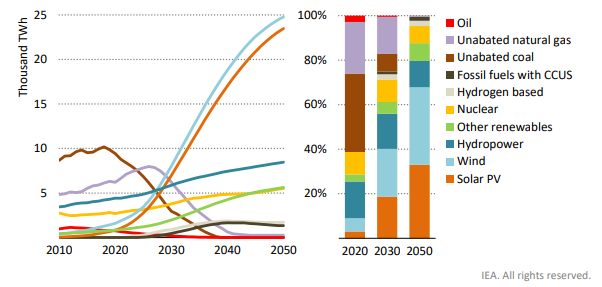
\includegraphics[width=0.8\textwidth]{Imagenes/NZE2050.png} \par\medskip
	
	\raggedright
	\footnotesize \textit{Nota.} Gráfico adaptado del reporte Net Zero Emissions by 2050 \citep{IEA_NZE_2021}.
	\label{fig:TendenciasNZE2050}
\end{figure}



En el ámbito nacional, la demanda energética peruana crece a un ritmo promedio del 3,5\,\% anual, con proyecciones sostenidas del 3\,\%, aunque evidencia una marcada disparidad regional \citep{ICEX2025}. Mientras que la zona centro reportó un incremento del 26\,\% en su demanda, las zonas norte y sur sufrieron contracciones del 36\,\% y 18\,\%, respectivamente.

En 2024, la producción eléctrica en el Perú alcanzó los 60.029 GWh, lo que supone un crecimiento del 3\,\%. Si bien la matriz nacional mantiene un sólido respaldo en fuentes hidráulicas y térmicas, las energías renovables no convencionales ganan terreno progresivamente \citep{ProActivo2025}. Para octubre de 2025, la generación mediante recursos renovables (solar, eólica, bagazo y biogás) creció un 27\,\% interanual, alcanzando el 13\,\% de la producción total. El objetivo estratégico del Estado es profundizar esta transición hasta que las energías limpias constituyan el 20\,\% de la matriz para el año 2030.

Las nuevas tendencias energéticas, lideradas por la tecnología solar fotovoltaica, plantean retos técnicos complejos para garantizar la eficiencia operativa \citep{XPower2024}. A medida que los proyectos fotovoltaicos escalan y se sitúan en terrenos topográficamente irregulares, factores como la variabilidad espacial de la irradiancia, las fluctuaciones térmicas, la suciedad y el ensombrecimiento afectan directamente la producción \citep{Salinas2025}. Bajo este escenario, la instrumentación rigurosa se convierte en un componente crítico \citep{SevenSensor}. El despliegue estratégico de redes de sensores, equipos de diagnóstico y plataformas de monitoreo continuo es indispensable para determinar el índice de rendimiento (\textit{Performance Ratio}) bajo normativas como la IEC 61724 \citep{IEC61724-1_2021}. Esta precisión no solo valida el diseño de la planta frente a la variabilidad climática, sino que habilita estrategias de mantenimiento predictivo capaces de anticipar anomalías, minimizar tiempos de inactividad y asegurar el retorno de inversión, consolidando a la energía solar como una infraestructura económica y resiliente \citep{Anatrac}.

\section{Definición de la problemática}

La implementación de instrumentación en plantas fotovoltaicas se enfrenta a un desafío logístico y técnico considerable: la heterogeneidad de las condiciones climáticas dentro de una misma instalación \citep{Salinas2025}. A medida que los proyectos a gran escala se asientan sobre terrenos con topografías complejas, como las vistas en la Figura \ref{fig:PlantaPeru}, se generan microclimas que provocan variaciones espaciales significativas. Por ejemplo, las diferencias de elevación alteran localmente los perfiles aerodinámicos del viento, mientras que las variaciones del albedo y el sombreado dinámico causan una distribución desigual de la radiación solar. Estudios en plantas de gran tamaño demuestran que esta dispersión geográfica puede generar diferencias de hasta un 20\,\% en la irradiación diaria y más del 40\,\% a nivel horario, así como variaciones térmicas de 6 a 7 °C entre paneles separados por unos pocos cientos de metros \citep{Garcia2014}.


\begin{figure}[H]
	% Fuerza la alineación izquierda y quita los ":" después del número
	\captionsetup{justification=raggedright, singlelinecheck=false, labelsep=none}
	
	\caption[Imagen aérea de planta de energía solar en inmediaciones de la fábrica de cemento Yura, Arequipa.]{} 
	
	\textit{Imagen aérea de planta de energía solar en inmediaciones de la fábrica de cemento Yura, Arequipa.} \par\medskip
	
	\centering
	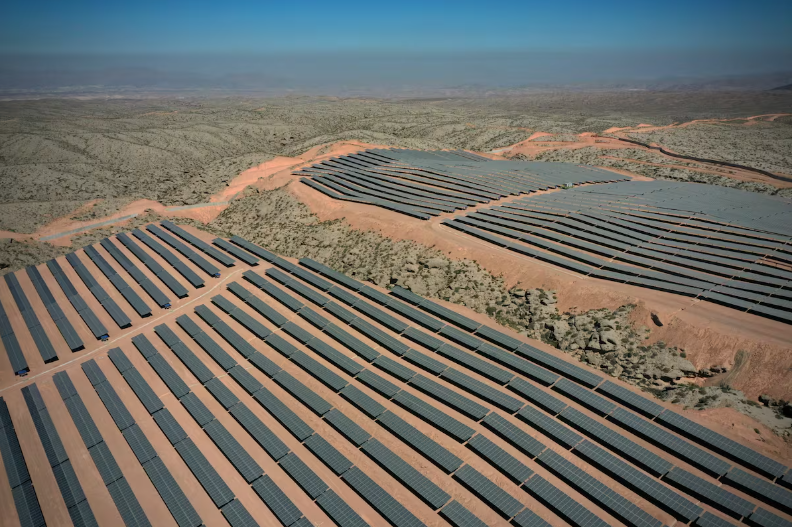
\includegraphics[width=0.6\textwidth]{Imagenes/PlantaPeru.png} \par\medskip
	
	\raggedright
	\footnotesize \textit{Nota.} Fotografía adaptada sobre la noticia ``Yura y el poder del sol'' \citep{YuraPeru}.
	\label{fig:PlantaPeru}
\end{figure}

Para hacer frente a esta variabilidad y cumplir con los requisitos de monitorización de normativas internacionales, como la IEC 61724-1 \citep{IEC61724-1_2021}, las plantas recurren actualmente a la instalación de estaciones  meteorológicas y redes de instrumentación fija. En el contexto de un parque fotovoltaico, una estación meteorológica se concibe como un núcleo de monitorización centralizado mediante un adquisidor de datos, el cual integra una serie de instrumentos de alta precisión para caracterizar el recurso solar y el entorno climático \citep{Anatrac}. Típicamente, esta estación está equipada con piranómetros, sensores de temperatura ambiente, anemómetros y medidores de humedad relativa y presión atmosférica.\citep{ProyectoEjecutivo2024}. Sin embargo, depender exclusivamente de puntos de medición estáticos presenta severas limitaciones. En la práctica, unos pocos sensores no logran capturar con precisión la variabilidad climática real a lo largo de terrenos extensos y con seguidores solares en dinámica constante \citep{Salinas2025}.

En consecuencia, el problema central se define como la ineficiencia de los métodos de instrumentación estáticos para caracterizar adecuadamente la variabilidad climática a lo largo de una planta fotovoltaica. Dado que resulta logísticamente inviable instalar estos instrumentos fijos en cada fila de paneles, los operadores se enfrentan a una alta incertidumbre en la evaluación de los índices de rendimiento energético y a deficiencias importantes para la detección y localización oportuna de fallas. 

A esta falta de representatividad espacial se suma el desafío financiero de intentar escalar o densificar la red de monitoreo, lo que representa gastos que llegan a constituir hasta el 1,6\,\% del presupuesto total de inversión de una planta fotovoltaica \citep{Burriana5MW}. Este conjunto de barreras evidencia la necesidad urgente de transitar hacia métodos de inspección dinámicos y verdaderamente representativos de todo el entorno solar.

%NOTA: AGREGAR MÁS CONSECUENCIAS, APARTE DE COSTOS, QUÉ MÁS?

\section{Propuesta de solución}
Para superar las limitaciones del monitoreo convencional, esta propuesta plantea el diseño y desarrollo de un robot autónomo especializado en la medición dinámica de variables climáticas dentro de sistemas fotovoltaicos. A diferencia de la infraestructura fija, este sistema funciona como una plataforma móvil adaptada para transportar instrumentos meteorológicos, lo que le permite realizar un barrido continuo en diversas secciones de la planta. Al desplazarse estratégicamente por el terreno, el robot recolecta datos que reflejan con mayor exactitud la dispersión geográfica de la irradiancia, los microclimas y las condiciones ambientales locales, con el fin de reducir el error en el cálculo y la estimación de la generación de energía, en cumplimiento con los métodos y exigencias de las normativas internacionales. Para complementar su funcionalidad, el sistema está diseñado para almacenar y transmitir toda la información capturada de forma inalámbrica, facilitando una plataforma de monitoreo remoto donde los operadores pueden visualizar el estado ambiental de la planta en tiempo real.


\subsection{Objetivos generales}

\subsubsection{Objetivo correspondiente a Trabajo de Fin de Carrera 1 (1MTR01)}
Elaborar el diseño conceptual y el anteproyecto de un robot autónomo para la medición de variables climáticas en sistemas fotovoltaicos.

\subsubsection{Objetivo para el proyecto general}
Desarrollar y elaborar el proyecto definitivo e implementar un prototipo del robot autónomo para la medición de variables climáticas en sistemas fotovoltaicos.

\subsection{Objetivos específicos}

\subsubsection{Objetivos correspondientes a Trabajo de Fin de Carrera 1 (1MTR01)}
\begin{itemize}
    \item Determinar los requerimientos funcionales, cinemáticos y de diseño del sistema mecatrónico a partir del análisis de las condiciones topográficas y climáticas en los parques solares.
    \item Desarrollar el diseño conceptual del sistema de locomoción, identificando sus funciones mecánicas y seleccionando los principios de tracción óptimos para garantizar un desplazamiento estable sobre terrenos irregulares.
    \item Desarrollar el diseño conceptual del mecanismo articulado, abstrayendo sus requerimientos cinemáticos y de actuación para asegurar la orientación independiente y precisa de los sensores climáticos.
    \item Estructurar la lógica del sistema de control autónomo, definiendo las funciones de procesamiento de señales, navegación y actuación requeridas para el seguimiento de rutas y la evasión de obstáculos.
    \item Plantear la arquitectura para el subsistema de telemetría y comunicaciones para garantizar la transmisión confiable de datos entre el robot y la central de control.
    \item Seleccionar el concepto de solución óptimo del sistema mediante una evaluación técnico-económica de las diferentes alternativas planteadas.
\end{itemize}

\subsubsection{Objetivos para el proyecto general}
\begin{itemize}
    \item Diseñar a detalle una base de transporte con alta capacidad de tracción, a partir del concepto mecánico seleccionado, para operar de manera estable sobre los terrenos irregulares que caracterizan a los parques solares.
    \item Diseñar una base móvil articulada e integrada al vehículo, basándose en la arquitectura óptima definida previamente, capaz de moverse y orientarse de forma independiente para adaptarse a la posición óptima requerida por los diversos sensores ambientales.
    \item Desarrollar un algoritmo de control autónomo, implementando la lógica estructurada en el diseño conceptual, que proporcione al vehículo la inteligencia necesaria para seguir rutas de inspección predefinidas y reaccionar ante imprevistos mediante la evasión de obstáculos.
    \item Implementar una infraestructura de comunicación inalámbrica, materializando el esquema tecnológico propuesto, utilizando paneles solares para energizar de forma autónoma los puntos independientes de comunicación, garantizando que los datos recolectados lleguen al centro de control sin interrupciones y permitiendo la intervención manual remota.
    \item Elaborar el proyecto definitivo del sistema incluyendo la elaboración de la lista de materiales, la estimación total de costos de implementación y la planificación de los protocolos de mantenimiento.
\end{itemize}

\section{Alcance y limitaciones}
El alcance de este proyecto y sus delimitaciones operativas se definen en conjunto a través de las siguientes características:

\begin{itemize}
    \item Abarca el diseño de detalle y la implementación de un prototipo físico o virtual de una base móvil robusta apta para desplazarse sobre los terrenos irregulares que caracterizan a las plantas fotovoltaicas.
    
    \item Incluye el desarrollo de la lógica y el algoritmo de control que permitirá al vehículo seguir rutas de inspección predefinidas y evadir obstáculos. No obstante, el desplazamiento se encuentra restringido por la morfología del suelo, limitando su operación a zonas con pendiente máxima del terreno de $14^\circ$.
    
    \item Comprende la incorporación de los instrumentos meteorológicos requeridos para monitorear las variables ambientales de forma dinámica. La precisión de esta instrumentación estará sujeta a factores ambientales, pudiendo verse mermada por el fenómeno del \textit{soiling} o presentar lecturas atípicas debido a sombras proyectadas y reflejos solares accidentales.
    
    \item La integridad mecánica, electrónica y de los sensores del sistema estará diseñada para soportar las altas exigencias climáticas de los parques solares, restringiendo su funcionamiento seguro a una temperatura ambiente máxima operativa de 45\,$^\circ$C.
    
    \item Contempla la implementación de un sistema de telemetría para almacenar y transmitir los datos medidos, habilitando la supervisión y el control remoto. Su desempeño dependerá estrictamente de la cobertura y estabilidad de la red inalámbrica existente en la instalación.
    
    \item La autonomía del robot estará directamente condicionada por la capacidad de su batería y su perfil de consumo energético, proyectándose una autonomía de operación continua de alrededor de 4 horas, lo que impone la necesidad de establecer ciclos de carga periódicos para mantener la continuidad del servicio en plantas que requieran un recorrido mayor al tiempo establecido..
\end{itemize}

\section{Metodología del diseño} 

El desarrollo del sistema mecatrónico se guiará por la directriz VDI 2221. Aunque la Ingeniería de Sistemas Basada en Modelos (MBSE) es una alternativa moderna que emplea modelos digitales formales para simular y analizar todo el ciclo de vida \citep{Isdefe2023}, su implementación requiere un ecosistema de software complejo orientado principalmente a sistemas de sistemas de alta criticidad. Por ello, se ha seleccionado la VDI 2221 para esta etapa del proyecto. En contraste con la MBSE, la norma VDI ofrece un enfoque pragmático y secuencial, perfectamente alineado con los objetivos del curso. De acuerdo con el cronograma del proyecto, el proceso se ha dividido en las siguientes fases:

\subsection{Definición de la tarea} 
Abarcada en los primeros avances del cronograma, esta fase involucra la recolección y el análisis exhaustivo de las condiciones operativas, topográficas y climáticas reales de los parques fotovoltaicos. Durante esta etapa se elabora el estado del arte, analizando las limitaciones de la instrumentación fija actual y los vehículos de inspección existentes. La fase culmina con la redacción de la lista de requerimientos, donde se determinan y cuantifican los requerimientos funcionales, cinemáticos y de diseño obligatorios para el sistema mecatrónico.

\subsection{Diseño conceptual} 
Desarrollada a través de entregas progresivas, esta fase materializa el enfoque modular establecido en los objetivos del proyecto. Inicia con la abstracción de la problemática mediante una caja negra y la definición de la estructura de funciones general. A partir de ello, el diseño se divide en los cuatro subsistemas clave: el sistema de locomoción, el mecanismo articulado, el sistema de control autónomo y el subsistema de telemetría y comunicaciones. Las funciones de estos subsistemas, a su vez, se clasifican en dominios. Para cada dominio se elaboran matrices morfológicas independientes. Finalmente, al integrar estos portadores de funciones, se proponen distintas alternativas conceptuales del robot, las cuales se someten a una evaluación técnico-económica para seleccionar el concepto de solución óptimo, presentando el anteproyecto a través de un modelo 3D.

\subsection{Diseño de detalle} 
Ubicada en la etapa de proyecto definitivo del cronograma, constituye la última etapa del desarrollo constructivo, en la cual se fijan con precisión las dimensiones, geometrías, presupuesto y la Lista de Materiales del sistema. Aquí se genera toda la documentación técnica requerida para la manufactura y puesta en marcha del robot autónomo, abarcando tres áreas clave: 

\begin{itemize} 
    \item \textbf{Dominio mecánico:} Elaboración de planos de fabricación, selección de materiales y dimensionamiento estructural definitivo tanto de la base móvil de tracción como de la base articulada de soporte para los sensores. 
    \item \textbf{Dominio electrónico y de energía:} Diseño de esquemáticos, enrutamiento de placas de circuito impreso, integración de la instrumentación de variables climáticas y dimensionamiento del sistema de alimentación independiente. 
    \item \textbf{Dominio de control y comunicaciones:} Desarrollo de la arquitectura de algoritmos para el seguimiento de rutas y evasión de obstáculos y diseño del enlace inalámbrico que garantizará la transmisión de datos al centro de monitoreo. 
\end{itemize}

\subsection{Implementación digital y validación}
Correspondiente a la etapa final de implementación del cronograma, esta fase se define de manera estrictamente digital, descartando la construcción física y enfocándose en el desarrollo de un prototipo virtual del diseño propuesto. Bajo este entorno digital, el proceso de validación se centrará única y exclusivamente en comprobar el sistema de comunicación inalámbrica. A través de herramientas de integración de red y simulación, se evaluará que el enlace de telemetría y la transmisión de los datos climáticos hacia la estación de monitoreo sean estables, asegurando que la arquitectura de red no sufra interrupciones y satisfaga todos los parámetros de conectividad estipulados en la lista de requerimientos.


%----------------------------------------------------------------------------------------
%	Capítulo 2
%----------------------------------------------------------------------------------------
\onehalfspacing
\fancypagestyle{plain}{
\fancyhf{}
\rhead{\thepage}
\renewcommand{\headrulewidth}{0pt}
\renewcommand{\footrulewidth}{0pt}
}

\chapter{COMPRENSIÓN DEL PROBLEMA}

\section{Marco teórico}

El presente marco teórico establece las bases físicas y conceptuales que fundamentan el estudio y justifican la necesidad de una monitorización climática dinámica. Comprender el comportamiento de los sistemas solares frente a las fluctuaciones ambientales es indispensable para evaluar su rendimiento real y superar las limitaciones espaciales que presentan los métodos de medición estáticos convencionales.

\subsection{Fundamentos de la conversión fotovoltaica}
La tecnología fotovoltaica se fundamenta en la conversión directa de la luz solar en electricidad mediante el efecto fotoeléctrico, utilizando como componente central celdas solares de materiales semiconductores, típicamente silicio, estructuradas internamente con una unión P-N, la cual es una unión física de un material semiconductor con huecos positivos (P) y con electrones negativos (N). A nivel físico, la radiación está compuesta por fotones; si la energía de estos impactos supera la banda de energía del material, logran liberar electrones de su estructura atómica. El campo eléctrico intrínseco de la celda se encarga entonces de separar estos portadores de carga, generando un movimiento direccionado que conforma una corriente continua lista para su aprovechamiento, transformación o almacenamiento \citep{martinez2018estimation}.

En la práctica, el rendimiento de esta conversión fotovoltaica no es un valor ideal fijo, sino que fluctúa en función de las condiciones meteorológicas del entorno operativo. Para predecir la potencia efectiva del sistema, se emplea un modelo matemático de estimación. Esta fórmula ajusta la potencia nominal estandarizada de fábrica considerando la cantidad real de luz solar incidente y las pérdidas por estrés térmico:

\begin{equation}
    P_{A} = P_{0} \frac{G_{i}}{1000} C_{K}
\end{equation}

donde:
\begin{itemize}
    \item $P_{0}$: Potencia máxima de instalación en condiciones estándar (W).
    \item $G_{i}$: Irradiancia global en el plano de la instalación ($W/m^{2}$).
    \item $C_{K}$: Factor de ajuste de potencia nominal por temperatura. Sin unidades. Calculado a través de la ecuación (9).
\end{itemize}

Dado que las condiciones estándar de prueba asumen una temperatura operativa ideal de 25 °C en la celda, el factor $C_{K}$ modela el cambio en la eficiencia cuando el panel tiene una temperatura diferente. Se calcula mediante la siguiente relación:

\begin{equation}
    C_{K} = 1 + \gamma_{P} * (T_{m} - 25)
\end{equation}

donde:
\begin{itemize}
    \item $\gamma_{P}$: Coeficiente relativo de temperatura. Entregado por el fabricante (en $\%.^{\circ}C^{-1}$).
    \item $T_{m}$: Temperatura del panel solar (en $^{\circ}C$).
\end{itemize}

Una vez que el sistema fotovoltaico ha sido montado, recibe luz solar y genera energía eléctrica. La combinación de valores de voltaje y corriente que puede entregar un sistema fotovoltaico se muestra en una gráfica denominada curva corriente contra voltaje (I-V). La Fig. 1-2 muestra una gráfica genérica, en la que la línea roja representa la curva I-V y la línea azul la relación de potencia total generada contra voltaje. Para generar la mayor cantidad de energía eléctrica se debe mantener el punto de operación cerca al punto de máxima potencia (MPP). Este punto corresponde a una combinación de valores entre la corriente de cortocircuito ($I_{SC}$) y el voltaje de circuito abierto ($V_{OC}$).

\subsection{Impacto de las variables meteorológicas y pérdidas técnicas}

El rendimiento de los sistemas fotovoltaicos no depende únicamente de sus especificaciones de diseño o fabricación, sino que está condicionado por las variaciones ambientales del entorno en el que operan. Cada instalación posee condiciones climáticas únicas que presentan desafíos diferentes para maximizar la eficiencia energética y optimizar las labores de mantenimiento \citep{chicaiza2024}.


\subsubsection{\textbf{Radiación solar:}} Representa el recurso energético primario. La radiación solar es directamente proporcional a la corriente generada por el panel fotovoltaico. Por lo tanto, cuando la irradiancia sube, la corriente de cortocircuito y la potencia máxima de salida del panel se incrementan \citep{Gonzalez2019Behavioral}. En la Figura \ref{fig:CurvasElectricasIrrTemp} (izquierda), se observa que, para un aumento de 600 a 1000~W/m$^{2}$, el valor de la corriente aumenta en cerca del 88\% para un mismo voltaje.
\subsubsection{\textbf{Temperatura ambiente:}} Influye de manera inversamente proporcional a la eficiencia de conversión debido a las propiedades termodinámicas del material semiconductor. A medida que la temperatura de la celda aumenta, el voltaje de circuito abierto disminuye. Esta caída de tensión provoca una reducción notable en la potencia máxima de salida. Por el contrario, en climas más fríos, la resistencia interna disminuye y el voltaje del panel tiende a aumentar \citep{Gonzalez2019Behavioral}. En la Figura \ref{fig:CurvasElectricasIrrTemp} (derecha), se observa que, para temperaturas de 25 °C y 55 °C, el valor de la potencia disminuye de 225 a 100~W (-55\%),

\begin{figure}[H]

	\captionsetup{justification=raggedright, singlelinecheck=false, labelsep=none}
	
	\caption[Comportamiento eléctrico de un panel solar ante variaciones de irradiancia y temperatura.]{} 
	
	\textit{Comportamiento eléctrico de un panel solar ante variaciones de irradiancia (izquierda) y temperatura (derecha).} \par\medskip
	
	\begin{minipage}{0.5\textwidth}
		\centering
		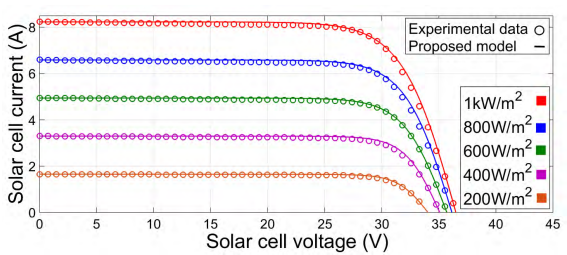
\includegraphics[width=\linewidth]{Imagenes/IEEE_V_Irr.png}
	\end{minipage}\hfill
	\begin{minipage}{0.5\textwidth}
		\centering
		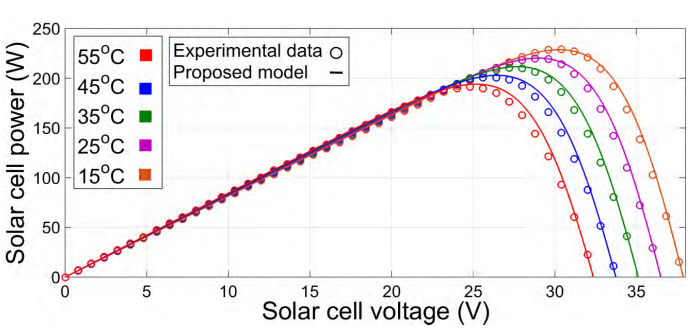
\includegraphics[width=\linewidth]{Imagenes/IEEE_T_Pwr.png}
	\end{minipage}
	\par\medskip
	
	\raggedright
	\footnotesize \textit{Nota.} Adaptado de \cite{Gonzalez2019Behavioral}.
	\label{fig:CurvasElectricasIrrTemp}
\end{figure}
    
\subsubsection{\textbf{Albedo:}} El albedo es la fracción de luz reflejada por el suelo, incide directamente en la cara posterior de los paneles bifaciales; un aumento en el índice de albedo eleva significativamente la corriente trasera, lo que genera una mayor ganancia bifacial y maximiza la producción total de energía del sistema \citep{Barreno2024}. En la Figura \ref{fig:CurvasElectricasAlbHum} (izquierda), se puede apreciar que, para todo el rango del coeficiente de albedo, la ganancia bifacial aumenta desde 5 a 25 \%.
    
\subsubsection{\textbf{Humedad y precipitaciones:}} Los altos niveles de humedad relativa aprovocan la refracción, reflexión y difracción de la luz solar. Esto atenúa la cantidad de radiación directa que logra alcanzar las celdas fotovoltaicas, reduciendo la corriente generada.   En contraste, aunque las precipitaciones reducen la irradiancia momentáneamente, actúan como el mecanismo de mitigación natural más efectivo, ya que lavan la superficie del panel, removiendo las partículas acumuladas causantes del \textit{soiling} \citep{Kazem2015Humidity}. En la Figura \ref{fig:CurvasElectricasAlbHum} (derecha), se observa que, para una diferencia de humedad del 30\% (entre 95 y 65 \%), el valor de la potencia aumenta de 50 a 105~W (+110\%),

\begin{figure}[H]
	
	\captionsetup{justification=raggedright, singlelinecheck=false, labelsep=none}
	
	\caption[Comportamiento eléctrico de un panel solar ante variaciones de albedo y humedad relativa.]{} 
	
	\textit{Comportamiento eléctrico de un panel solar ante variaciones de albedo (izquierda) y humedad relativa (derecha).} \par\medskip
	
	\begin{minipage}{0.5\textwidth}
		\centering
		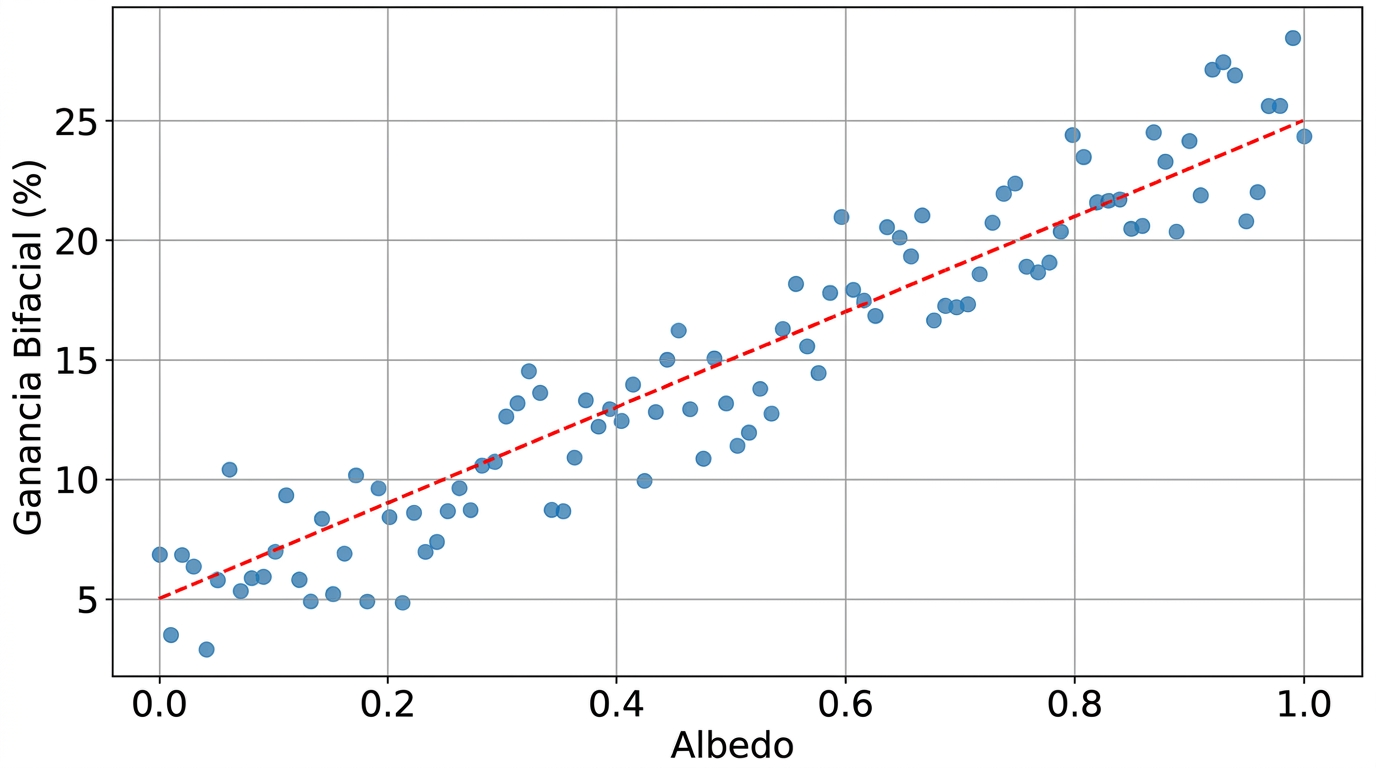
\includegraphics[width=\linewidth]{Imagenes/BARRENO_Alb_Ganancia.jpeg}
	\end{minipage}\hfill
	\begin{minipage}{0.5\textwidth}
		\centering
		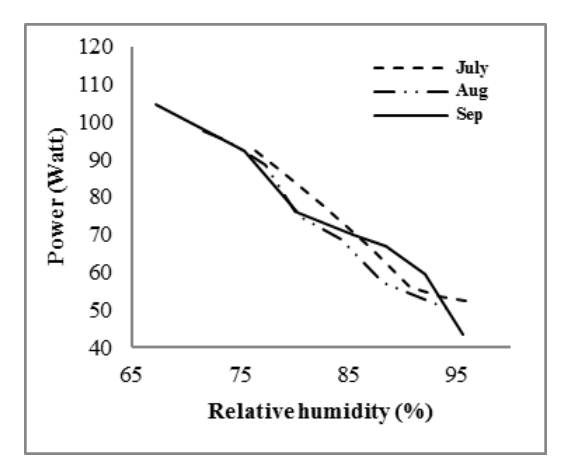
\includegraphics[width=\linewidth]{Imagenes/KAZEM_Hum_Pwr.png}
	\end{minipage}
	\par\medskip
	
	\raggedright
	\footnotesize \textit{Nota.} Adaptado de \cite{Barreno2024} (izquierda).Adaptado de \cite{Kazem2015Humidity} (derecha).
	\label{fig:CurvasElectricasAlbHum}
\end{figure}


\subsubsection{\textbf{Velocidad del viento:}} Presenta un efecto dual. Por un lado, cuando la velocidad del viento es moderada, este favorece el enfriamiento convectivo de los paneles, disipando el calor acumulado y reduciendo la temperatura de la celda, lo que incrementa la eficiencia y la potencia eléctrica de salida. 
Por otro lado, las ráfagas actúan como el principal transporte de partículas. Esto eleva las tasas de deposición de suciedad sobre los cristales, disminuyendo la generación de energía \citep{Vick_WindEffect}. En la Figura \ref{fig:Leow_Wind_Pwr} (derecha), se observa un una comparación cualitativa de la potencia de salida de dos paneles solares, con una diferencia promedio a lo largo de día de 7~W (11\% de potencia máxima de panel con aire).
    
\begin{figure}[H]
	\captionsetup{justification=raggedright, singlelinecheck=false, labelsep=none}
	\caption[Comparación entre la potencia generada a lo largo del día de paneles con y sin velocidad de viento.]{} 
	\textit{Comparación entre la potencia generada a lo largo del día de paneles con y sin velocidad de viento.} \par\medskip
	
	\centering
	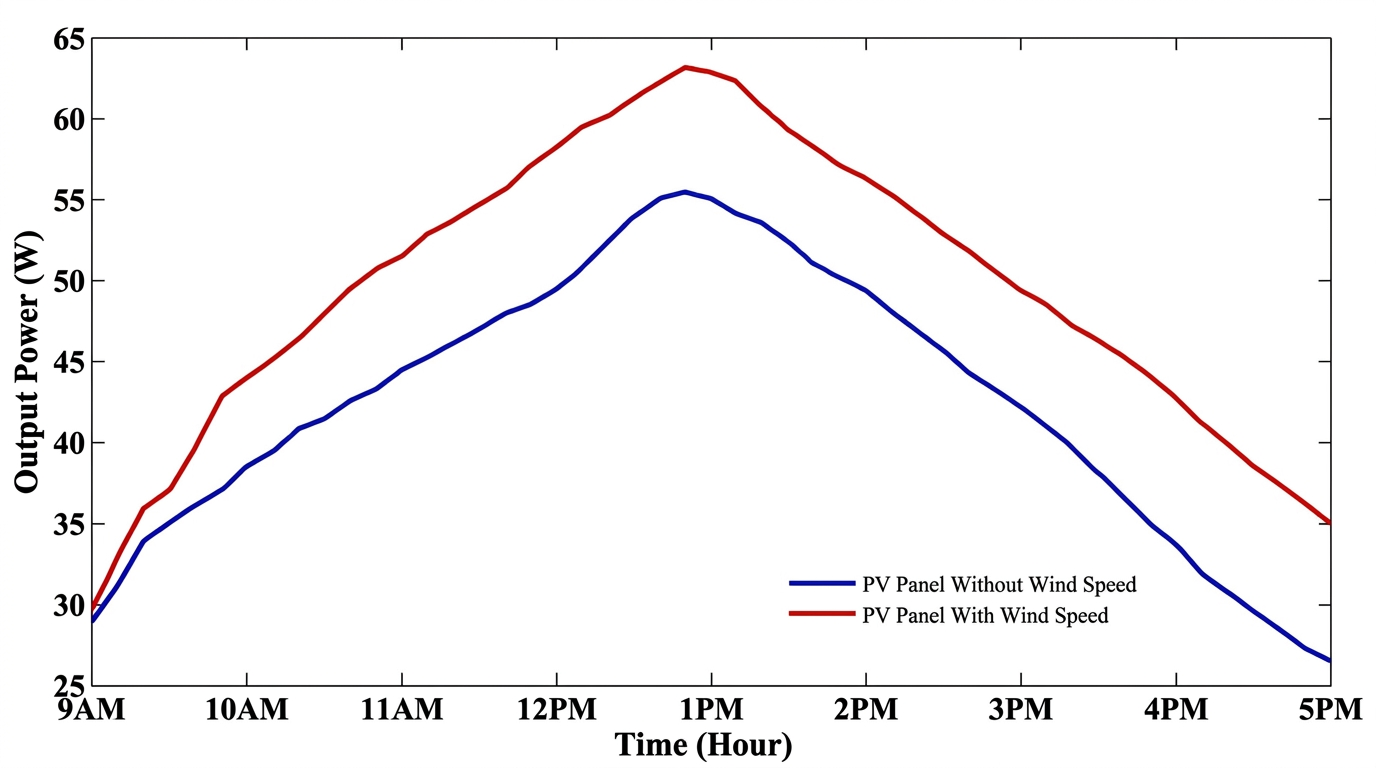
\includegraphics[width=0.8\textwidth]{Imagenes/Leow_Wind_Pwr.jpeg} \par\medskip
	\raggedright
	\footnotesize \textit{Nota.} Gráfico adaptado del artículo ``Influence of wind speed on the performance of photovoltaic
	panel'' \citep{Leow2019Wind}.
	\label{fig:Leow_Wind_Pwr}
\end{figure}

\subsubsection{\textbf{Pérdidas Técnicas:}} La eficiencia de esta conversión disminuye significativamente bajo condiciones operativas reales debido a dos fenómenos físicos principales. En primer lugar, el efecto térmico provoca que las celdas solares pierdan eficiencia a medida que su temperatura aumenta, ya que dicho incremento genera un coeficiente negativo en el voltaje de circuito abierto que reduce drásticamente la potencia máxima de salida \citep{Vieira2024}. 
Por otro lado, el fenómeno del soiling consiste en la acumulación de polvo, arena y contaminantes sobre la superficie de los módulos; esta capa de suciedad interfiere con la transmisión de la luz mediante procesos de absorción, reflexión y dispersión, generandopérdidas eléctricas que, al distribuirse de forma no uniforme, pueden derivar en la formación de puntos caliente” perjudiciales para la vida útil del panel y reducir severamente la rentabilidad de la instalación \citep{TesisJGB}.

\section{Marco referencial}

En esta sección se detallan las normativas, las condiciones topográficas y el entorno operativo bajo los cuales funcionará el robot autónomo de medición.

\subsection{Contexto normativo y estándares de medición}
Dado que el objetivo del vehículo es recolectar datos climáticos con validez industrial para el cálculo de índices de rendimiento, su instrumentación y métodos deben regirse estrictamente por la serie de estándares internacionales IEC 61724. Esta familia de normativas es la base para evaluar la capacidad y la energía de los sistemas fotovoltaicos. Dentro de esta serie, el principal referente para el diseño del hardware es la norma IEC 61724-1, la cual establece los requisitos para la monitorización del desempeño de sistemas fotovoltaicos y define las clases de exactitud exigidas para los sensores de irradiancia, temperatura y condiciones ambientales. Las exigencias de los parámetros más críticos definidos por esta norma, junto con su impacto en el proyecto, se detallan a continuación en la Tabla \ref{tab:requisitos_clase_ab}.

\begin{center}
\footnotesize
\begin{xltabular}{\textwidth}{|p{1.8cm}|>{\raggedright\arraybackslash}X|>{\raggedright\arraybackslash}X|p{2.8cm}|p{2.8cm}|}
\caption{Requisitos detallados por la Norma IEC 61724-1.}
\label{tab:requisitos_clase_ab} \\
\hline
\rowcolor[HTML]{D9E1F2} 
 &  &  & \multicolumn{2}{c|}{\textbf{Rango definido por la norma}} \\ \cline{4-5} 
\rowcolor[HTML]{D9E1F2} 
\multirow{-2}{*}{\textbf{Parámetro}} & \multirow{-2}{*}{\textbf{Descripción}} & \multirow{-2}{*}{\textbf{Impacto}} & \textbf{Clase A} & \textbf{Clase B} \\ \hline
\endfirsthead

\multicolumn{5}{c}%
{{\bfseries Continuación de la \tablename\ \thetable{}}} \\
\hline
\rowcolor[HTML]{D9E1F2} 
\textbf{Parámetro} & \textbf{Descripción} & \textbf{Impacto} & \textbf{Clase A} & \textbf{Clase B} \\ \hline
\endhead

\hline
\endfoot

\hline
\endlastfoot

\textbf{Clasificación} & Define las exigencias de exactitud y el diseño general para la recolección de datos. & Determina el rigor técnico y económico de la monitorización. & Alta exactitud (plantas grandes o a escala de red). & Exactitud media (instalaciones comerciales pequeñas o medianas). \\ \hline

\textbf{Intervalos} & Frecuencia de adquisición física (muestreo) y almacenamiento (registro). & Una alta frecuencia captura fluctuaciones rápidas y reduce la incertidumbre. & Muestreo máximo cada 5 segundos; Registro máximo cada 5 minutos, recomendado cada 1 minuto.. & Muestreo máximo cada 1 minuto; Registro máximo cada 5 minutos. \\ \hline

\textbf{Irradiancia} & Exigencias para los sensores de radiación incidente frontal y posterior. & Su exactitud define la incertidumbre final de la auditoría de rendimiento. & Piranómetro Clase A, espectralmente plano, incertidumbre menor al 2\%. & Piranómetro Clase C, incertidumbre menor al 3\%. \\ \hline

\textbf{Temperatura} & Medición térmica en la cara posterior del módulo y del aire circundante. & Dato vital para el cálculo de eficiencia corregido por temperatura. & \multicolumn{2}{p{5.6cm}|}{Resolución menor a $0,1^{\circ}\text{C}$ e incertidumbre entre $ \pm 1^{\circ}\text{C}$. El sensor de ambiente debe estar a 1 metro de distancia de fuentes térmicas.} \\ \hline

\textbf{Mitigación ambiental} & Protocolos de limpieza (\textit{soiling}) y sistemas contra rocío o escarcha. & Evita mediciones artificialmente bajas que afectarían el índice de rendimiento. & \multicolumn{2}{p{5.6cm}|}{Limpieza semanal o uso de tecnología automatizada de detección de \textit{soiling}} \\ \hline


\textbf{Salida de planta} & Medidor principal de potencia y energía neta inyectada a la red. & Determina el cumplimiento de garantías y la facturación real. & Medidores de Clase 0.2 S. & Medidores de Clase 0.5 S. \\ \hline

\end{xltabular}
\end{center}

\subsection{Condiciones topográficas y geográficas}
Las plantas solares a gran escala se pueden instalar en terrenos irregulares y montañosos que presentan una topografía compleja, lo cual propicia la generación de microclimas y fluctuaciones espaciales en la radiación incidente. El diseño de la base móvil y el sistema de locomoción del robot están directamente condicionados por las severas exigencias de este entorno natural; como los desniveles pronunciados, que pueden alcanzar hasta un 25\,\% \citep{Salinas2025}, como se puede observar en la Figura \ref{fig:PlantaPendiente} ; o los obstáculos geológicos, que incluye maleza, arena suelta, rocas, zanjas profundas causas por erosión y charcos de lodo \citep{Figgis2025}. Estas complejas condiciones justifican la adopción de sistemas de tracción con alta adaptabilidad y agarre, como los sistemas de orugas, necesarios para superar áreas inestables.

\begin{figure}[H]
	% Fuerza la alineación izquierda y quita los ":" después del número
	\captionsetup{justification=raggedright, singlelinecheck=false, labelsep=none}
	
	\caption[Imagen aérea de varias colinas cubiertas con paneles fotovoltaicos en Jinhua, provincia de Zhejiang, China.]{} 
	
	\textit{Imagen aérea de varias colinas cubiertas con paneles fotovoltaicos en Jinhua, provincia de Zhejiang, China.} \par\medskip
	
	\centering
	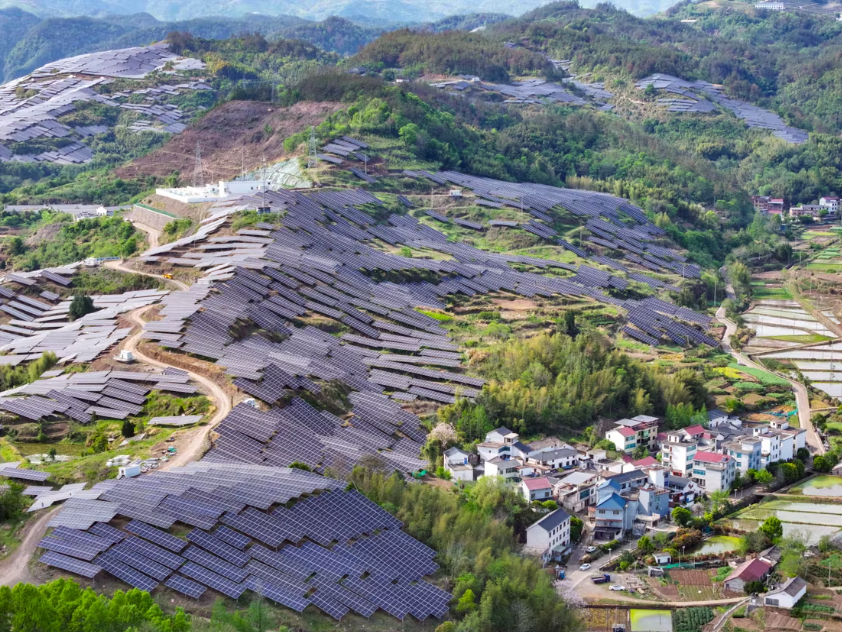
\includegraphics[width=0.6\textwidth]{Imagenes/PlantaPendiente.png} \par\medskip
	
	\raggedright
	\footnotesize \textit{Nota.} Fotografía adaptada sobre la noticia ``China, the energy transition superpower''  \citep{Pouille2025China}.
	\label{fig:PlantaPendiente}
\end{figure}

\subsection{Entorno operativo y tecnológico}
El contexto operativo y tecnológico define las estrechas interacciones del vehículo autónomo con la infraestructura civil y electromecánica propia de la planta. El trazado de las instalaciones modernas se apoya mayoritariamente en estructuras con seguidores solares de un solo eje, orientados de norte a sur y separados por pasillos que oscilan entre los 5 y 9 
de distancia \citep{ProyectoEjecutivo2024}.

En este escenario, la navegación autónoma del robot se verá restringida por obstáculos artificiales críticos. Entre ellos, la reducción del espacio transitable por la instalación de bandejas de distribución de cables y mallas reflectantes en el suelo, y la presencia de barras mecánicas entre las filas de los seguidores solares que impiden el libre tránsito transversal entre pasillos \citep{Figgis2025}. Todo ello exige que el robot disponga de un sistema de evitación de obstáculos robusto y una extrema precisión en su desplazamiento.

\section{Estado del arte} %PONER IMÁGENES EN LA TABLA

\subsection{Soluciones integrales}
En esta sección se analizan los sistemas mecatrónicos completos que intentan resolver el problema general de la inspección y medición dentro de los parques solares fotovoltaicos, sirviendo como referentes de diseño global para el vehículo terrestre autónomo propuesto.

\subsubsection{\textbf{Estación meteorológica fotovoltaica móvil (CN 216956405 U):}} Esta patente describe, como se ilustra en la Figura \ref{fig:CN216956405U} (izquierda), una estación climática (2) montada sobre una base con ruedas, vista en Figura la \ref{fig:CN216956405U} (derecha), que incluye soportes roscados, compuestos por una funda roscada y una varilla roscada, y placas o almohadillas estabilizadoras (5) que se despliegan hacia abajo para anclar el equipo en superficies desniveladas. El sistema destaca por su enfoque en la estabilización mecánica del equipo de medición, utilizando estos mecanismos de anclaje desplegables que aseguran que los sensores meteorológicos mantengan un plano de referencia adecuado al evitar que la base se incline, así como evita volcaduras el recorrido en terrenos con pendiente.
	
	\begin{figure}[H]
		
		\captionsetup{justification=raggedright, singlelinecheck=false, labelsep=none}
		
		\caption[Ilustraciones de estación meteorológica fotovoltaica móvil.]{} 
		
		\textit{Ilustraciones de estación meteorológica fotovoltaica móvil.} \par\medskip
		
		\begin{minipage}{0.4\textwidth}
			\centering
			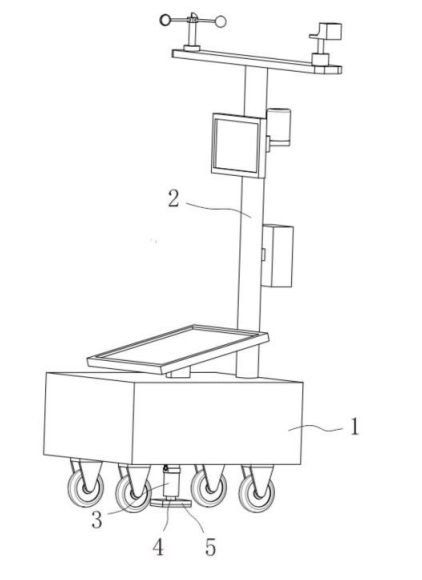
\includegraphics[width=\linewidth]{Imagenes/CN216956405U-1.png}
		\end{minipage}\hfill
		\begin{minipage}{0.4\textwidth}
			\centering
			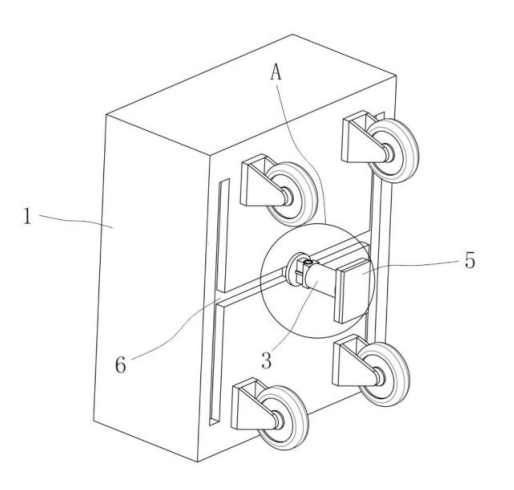
\includegraphics[width=\linewidth]{Imagenes/CN216956405U-2.png}
		\end{minipage}
		\par\medskip
		
		\raggedright
		\footnotesize \textit{Nota.} Adaptado de \cite{CN216956405U}.
		\label{fig:CN216956405U}
	\end{figure}
	
	
\subsubsection{\textbf{Vehículo de inspección para plantas de energía fotovoltaicas (CN 218409341 U):}} Es un vehículo terrestre no tripulado, mostrado en la Figura \ref{fig:CN218409341U}, montado sobre una base (1), equipado con ruedas de movimiento (21), paneles solares abatibles (12) para carga y un robusto mecanismo de amortiguación mediante resortes (20) en cajas para evitar daños en la instrumentación durante el tránsito. Esta patente representa una solución integral para la problemática, implementando el uso de paneles solares integrados para la recarga autónoma y sistemas de amortiguación para la protección de la instrumentación, lo que aseguraa la precisión de las mediciones dinámicas y prolonga la autonomía.
	
	\begin{figure}[H]
		\captionsetup{justification=raggedright, singlelinecheck=false, labelsep=none}
		
		\caption[Ilustración de vehículo de inspección con paneles solares y sistema de amortiguación.]{} 
		
		\textit{Ilustración de vehículo de inspección terrestre con paneles solares abatibles y mecanismo de amortiguación.} \par\medskip
		
		\centering
		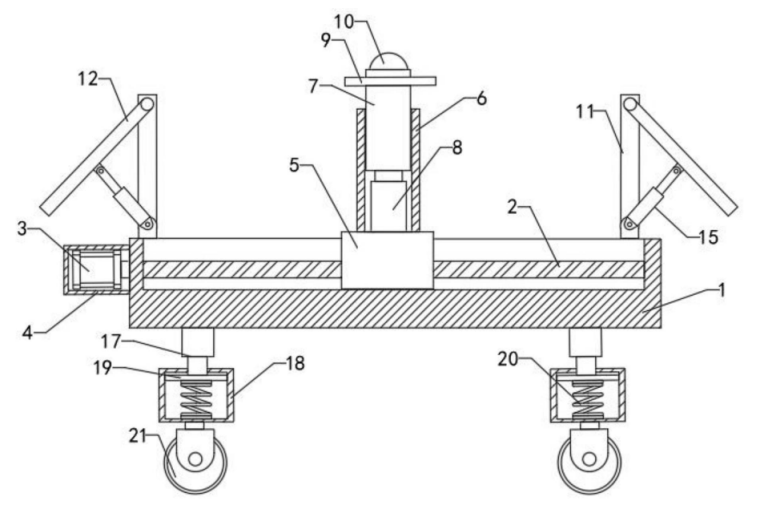
\includegraphics[width=0.75\textwidth]{Imagenes/CN218409341U.png} \par\medskip
		
		\raggedright
		\footnotesize \textit{Nota.} Adaptado de \cite{CN218409341U}.
		\label{fig:CN218409341U}
	\end{figure}
\subsubsection{\textbf{Vehículo de inspección para plantas fotovoltaicas en desiertos (CN 221163061 U):}} 
Este robot, como se ilustra en la Figura \ref{fig:CN221163061U}, cuenta con tracción de orugas (2) diseñada con ángulos de inclinación anti-deslizamiento (22) y está equipado con radar y sensores de viento, humedad y radiación o luz. La propuesta se alinea con el propósito general del proyecto, ya que el diseño integrado de un tren de tracción para terrenos desérticos acoplado a un sistema completo de sensores climáticos sirve como el principal punto de referencia comercial y tecnológico para validar la arquitectura y el alcance funcional del UGV de irradiancia propuesto.
	
	\begin{figure}[H]
		\captionsetup{justification=raggedright, singlelinecheck=false, labelsep=none}
		
		\caption[Ilustración de robot de inspección para estaciones fotovoltaicas en el desierto.]{} 
		
		\textit{Ilustración de robot de inspección con tracción de orugas y sensores climáticos para entornos desérticos.} \par\medskip
		
		\centering
		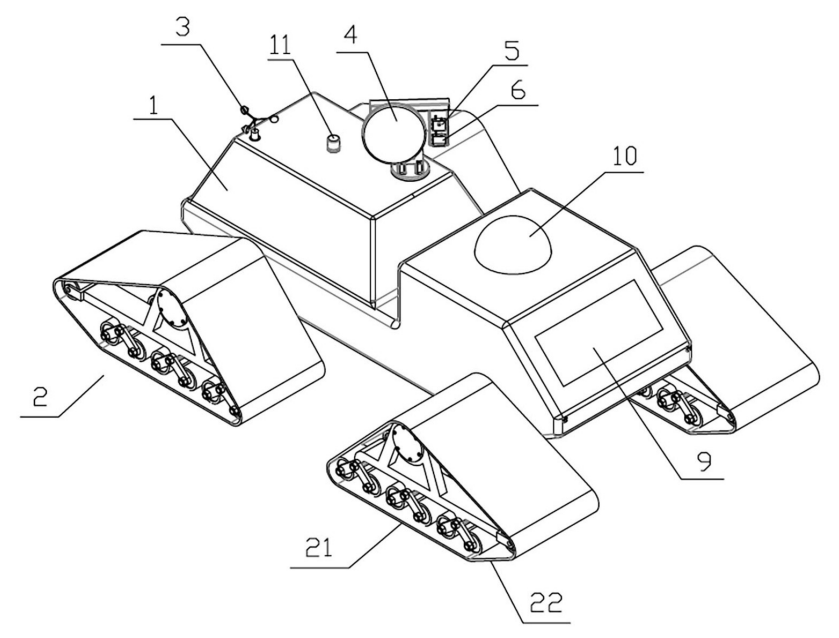
\includegraphics[width=0.7\textwidth]{Imagenes/CN221163061U.png} \par\medskip
		
		\raggedright
		\footnotesize \textit{Nota.} Adaptado de \citep{CN221163061U}.
		\label{fig:CN221163061U}
	\end{figure}
%%
%%
\begin{center}
\footnotesize
\begin{xltabular}{\textwidth}{|p{2.5cm}|>{\raggedright\arraybackslash}X|>{\raggedright\arraybackslash}X|>{\raggedright\arraybackslash}X|}
\caption{Análisis comparativo de Soluciones Integrales.}
\label{tab:estado_arte_integrales} \\
\hline
\rowcolor[HTML]{D9E1F2} 
\textbf{Referente} & \textbf{Principio de Funcionamiento} & \textbf{Aporte al Proyecto} & \textbf{Limitaciones} \\ \hline
\endfirsthead

\multicolumn{4}{c}%
{{\bfseries Continuación de la \tablename\ \thetable{}}} \\
\hline
\rowcolor[HTML]{D9E1F2} 
\textbf{Referente} & \textbf{Principio de Funcionamiento} & \textbf{Aporte al Proyecto} & \textbf{Limitaciones} \\ \hline
\endhead

\hline
\endfoot

\hline
\endlastfoot

%%
%%
%%

Estación meteorológica fotovoltaica móvil (CN 216956405 U)  & Estación sobre ruedas que emplea soportes roscados y almohadillas estabilizadoras de despliegue mecánico. & Proporciona mecanismos de nivelación y estabilización para asegurar el plano horizontal durante la lectura estática de sensores. & Tracción por ruedas ineficiente en terrenos irregulares; la nivelación pausada ralentiza el proceso de inspección dinámica. \\ \hline

Vehículo de inspección para plantas de energía fotovoltaicas (CN 218409341 U)  & Vehículo terrestre (UGV) con paneles solares abatibles y un mecanismo robusto de amortiguación con resortes en cajas. & Extiende la autonomía energética del robot e incorpora suspensión vital para proteger instrumentos sensibles de las vibraciones. & Locomoción por ruedas; carece de actuadores o mecanismos para limpiar los instrumentos ante la acumulación de polvo. \\ \hline

Vehículo de inspección para plantas fotovoltaicas en desiertos (CN 221163061 U)  & Chasis hermético propulsado por orugas antideslizantes, equipado con radar y sensores de radiación, viento y humedad. & Modelo de arquitectura mecatrónica base para un UGV desértico, combinando alta movilidad con medición climatológica. & Instrumentación estática en el chasis; no cuenta con ejes para adaptar la elevación o inclinación de los sensores a los paneles. \\ \hline

\end{xltabular}
\end{center}

%%
%%
\vspace{-1.5cm}
%%
\subsection{Soluciones parciales}
En esta sección se describen los componentes y subsistemas especializados que abordan necesidades técnicas específicas, clasificados según su funcionalidad.

\subsubsection{Robots para plantas fotovoltaicas}
\begin{itemize}
	\item \textbf{Vehículo de inspección terrestre inteligente para plantas fotovoltaicas (CN 119665962 A):} Esta patente, ilustrada en la Figura \ref{fig:CN119665962A&CN120057153A} (izquierda), describe un vehículo terrestre no tripulado cuya base (10) que incorpora soportes (20) y una carcasa superior (40) que aloja un panel fotovoltaico (30). Este vehículo está diseñado para la generación de mapas espaciales y la planificación de rutas globales de forma autónoma. El sistema integra algoritmos de navegación y percepción que le permiten realizar la recolección de datos ambientales en movimiento y la evasión de obstáculos en el terreno de manera autónoma.
	
	\item \textbf{Robot de inspección de alta transitabilidad para plantas fotovoltaicas (CN 120057153 A):} Ilustrado en la Figura \ref{fig:CN119665962A&CN120057153A} (derecha), se trata de un vehículo con tracción mediante ruedas activas (31) (con opción de incluir configuraciones de oruga) conectadas a módulos flotantes (32) de amortiguación con resortes oscilantes (35). Este diseño está concebido para operar en entornos con topografía irregular, como suelo desértico o con pendientes pronunciadas. Su configuración mecánica también incluye un brazo base (4) desplegable desde un compartimento de almacenamiento (2) para labores de inspección, el cual garantiza la estabilidad y movilidad del robot frente a obstáculos comunes en las plantas solares a gran escala, permitiéndole navegar entre los paneles incluso cuando la distancia al suelo es reducida.
	
	
	\begin{figure}[H]
		
		\captionsetup{justification=raggedright, singlelinecheck=false, labelsep=none}
		
		\caption[Ilustraciones de vehículo de inspección terrestre inteligente y robot de inspección de alta transitabilidad.]{} 
		
		\textit{Ilustraciones de vehículo de inspección terrestre inteligente y robot de inspección de alta transitabilidad.} \par\medskip
		
		\begin{minipage}{0.6\textwidth}
			\centering
			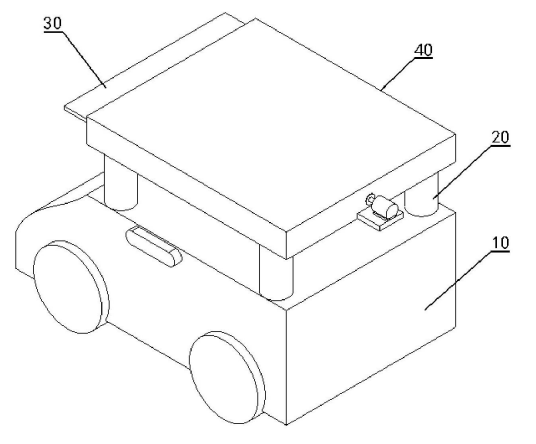
\includegraphics[width=\linewidth]{Imagenes/CN119665962A.png}
		\end{minipage}\hfill
		\begin{minipage}{0.5\textwidth}
			\centering
			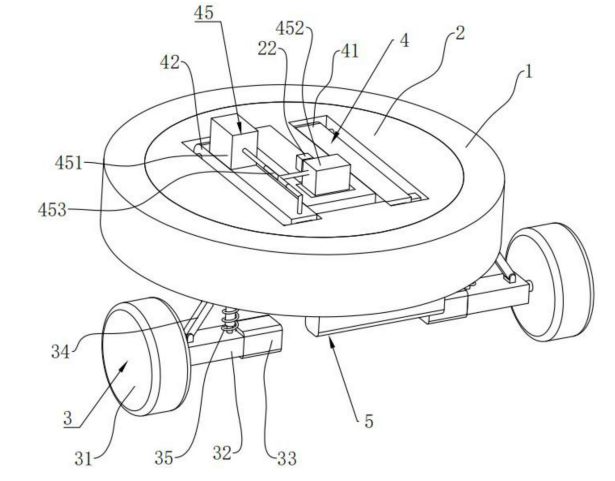
\includegraphics[width=\linewidth]{Imagenes/CN120057153A.png}
		\end{minipage}
		\par\medskip
		
		\raggedright
		\footnotesize \textit{Nota.} Adaptado de \cite{CN119665962A} (izquierda) y \cite{CN120057153A} (derecha).
		\label{fig:CN119665962A&CN120057153A}
	\end{figure}
	
	\item \textbf{Dispositivo de inspección automática para plantas fotovoltaicas (CN 220873036 U):} Este robot móvil, ilustrado en la Figura \ref{fig:CN220873036U}, comprende un cuerpo (1) sobre un mecanismo de desplazamiento, destaca por incorporar un motor (17) y un brazo giratorio o varilla (18) equipado con un cepillo o esponja (19) automatizado para la limpieza de los lentes de sus cámaras y mecanismos de captura de imágenes (8). Esta solución mecatrónica es esencial para mitigar el impacto del \textit{soiling} en los propios instrumentos del vehículo, como la plataforma de imágenes infrarrojas, asegurando la correcta lectura en las mediciones meteorológicas durante operaciones prolongadas en entornos con mucho polvo.
	
	\begin{figure}[H]
		\captionsetup{justification=raggedright, singlelinecheck=false, labelsep=none}
		
		\caption[Ilustración de vehículo de inspección con sistema de limpieza de sensores]{} 
		
		\textit{Ilustración de dispositivo de inspección automática con mecanismos de limpieza para sus instrumentos ópticos.} \par\medskip
		
		\centering
		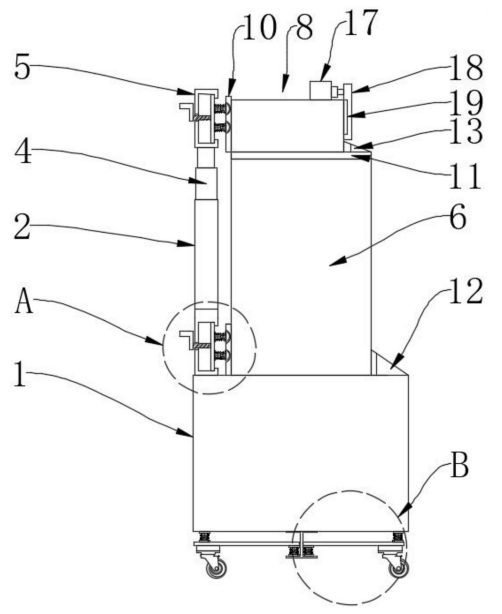
\includegraphics[width=0.4\textwidth]{Imagenes/CN220873036U.png} \par\medskip
		
		\raggedright
		\footnotesize \textit{Nota.} Adaptado de \cite{CN220873036U}.
		\label{fig:CN220873036U}
	\end{figure}
\end{itemize}

\begin{table}[H]
	\centering
	\footnotesize
	\caption{Análisis comparativo de Soluciones Parciales: Robots para plantas fotovoltaicas.}
	\label{tab:estado_arte_robots_pv}
	\begin{tabularx}{\textwidth}{|p{3.5cm}|>{\raggedright\arraybackslash}X|>{\raggedright\arraybackslash}X|>{\raggedright\arraybackslash}X|}
		\hline
		\rowcolor[HTML]{D9E1F2} 
		\textbf{Referente} & \textbf{Principio de Funcionamiento} & \textbf{Aporte al Proyecto} & \textbf{Limitaciones} \\ \hline
		Vehículo de inspección terrestre inteligente para plantas fotovoltaicas (CN 119665962 A) & Emplea algoritmos de control y datos ambientales para generar mapas espaciales y trazar rutas. & Aporta la arquitectura lógica para la navegación autónoma global y la evasión dinámica de obstáculos en la planta. & Cubre únicamente el dominio de software y control; no soluciona los retos mecánicos de tracción ni de captura física de datos. \\ \hline
		Robot de inspección de alta transitabilidad para plantas fotovoltaicas (CN 120057153 A) & Tren de locomoción basado en orugas acoplado a módulos flotantes de amortiguación para mantener el equilibrio. & Diseño mecánico ideal para sortear terrenos muy complejos, zanjas erosivas y pendientes de arena suelta. & Enfoque puramente cinemático y estructural; no integra sistemas de comunicación o instrumentación meteorológica. \\ \hline
		Dispositivo de inspección automática para plantas fotovoltaicas (CN 220873036 U) & Brazo robótico automatizado equipado con esponja o cepillo para frotar y limpiar los lentes de a bordo. & Estrategia de interacción física para mitigar de forma activa el soiling en los instrumentos durante largos recorridos. & Sistema optimizado para cámaras frontales; requiere rediseño para no dañar los domos de vidrio de los piranómetros. \\ \hline
	\end{tabularx}
\end{table}

\subsubsection{Robots para inspección de plantas de energía}
\begin{itemize}
	\item \textbf{Robot de inspección inteligente para plantas de energía (CN 215511023 U):} Esta plataforma móvil de orugas, como se ilustra en la Figura \ref{fig:CN215511023U&CN215701759U} (izquierda), integra un brazo mecánico (4) y un sistema de visión compuesto por una cámara óptica y un sensor infrarrojo. Una característica innovadora de este diseño es la inclusión de un sensor de nivel de líquidos (8) en su parte inferior, lo que permite al vehículo detectar y evadir charcos de lodo o zonas inundadas para proteger la integridad de sus componentes electrónicos, como el host de control central (7).
	
	\item \textbf{Robot de inspección para plantas de energía con mecanismo de corte (CN 215701759 U):} Este vehículo, como se ilustra en la Figura \ref{fig:CN215511023U&CN215701759U} (derecha) está equipado con un brazo giratorio (7) que posee un motor (8) y aspas de corte integradas (9). Este mecanismo permite al robot abrirse paso a través de vegetación o maleza que pueda obstruir las rutas de inspección, garantizando la continuidad del servicio de mantenimiento.
	
	
		\begin{figure}[H]
		
		\captionsetup{justification=raggedright, singlelinecheck=false, labelsep=none}
		
		\caption[Ilustraciones de robot de inspección con sensor de líquidos y robot de inspección con mecanismo de corte de maleza.]{} 
		
		\textit{Ilustraciones de robot de inspección con sensor de líquidos y robot de inspección con mecanismo de corte de maleza.} \par\medskip
		
		\begin{minipage}{0.5\textwidth}
			\centering
			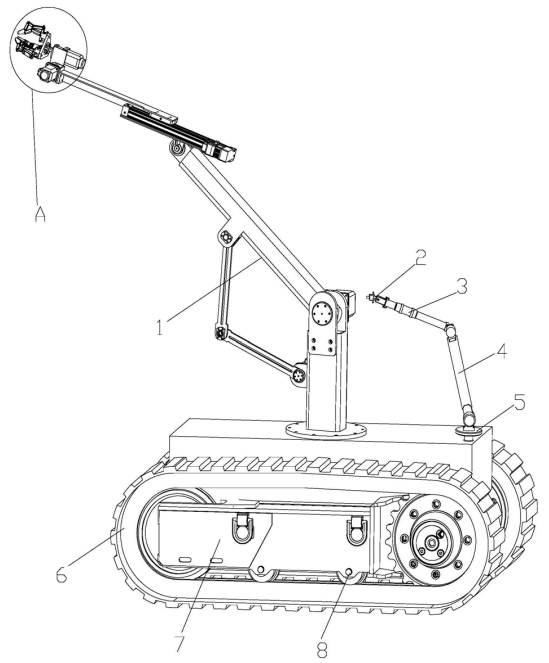
\includegraphics[width=\linewidth]{Imagenes/CN215511023U.png}
		\end{minipage}\hfill
		\begin{minipage}{0.6\textwidth}
			\centering
			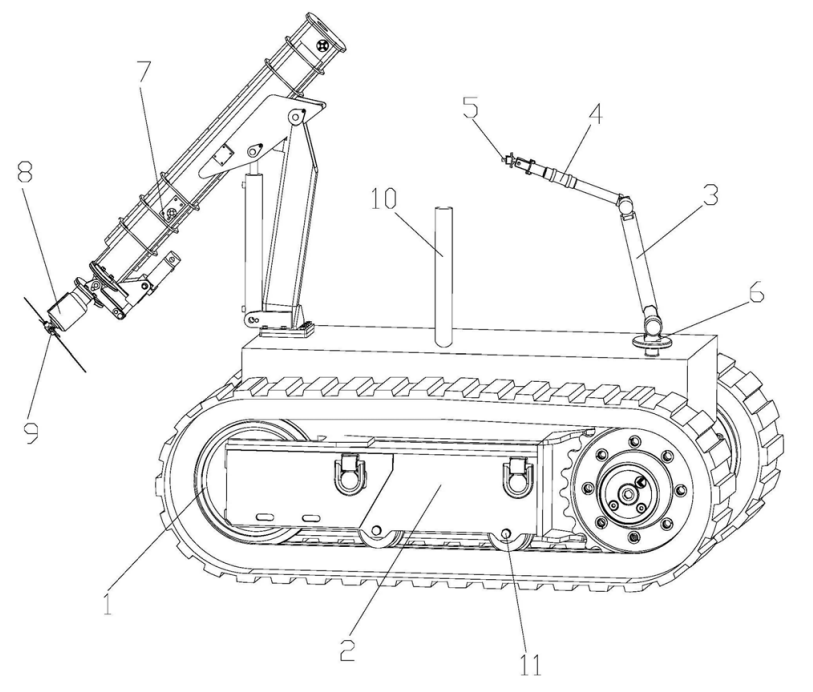
\includegraphics[width=\linewidth]{Imagenes/CN215701759U.png}
		\end{minipage}
		\par\medskip
		
		\raggedright
		\footnotesize \textit{Nota.} Adaptado de \cite{CN215511023U} (izquierda) y \cite{CN215701759U} (derecha).
		\label{fig:CN215511023U&CN215701759U}
	\end{figure}
	
	
	
\end{itemize}
%%%%%%

\begin{table}[H]
	\centering
	\footnotesize
	\caption{Análisis comparativo de Soluciones Parciales: Robots para inspección en general.}
	\label{tab:estado_arte_robots_general}
	\begin{tabularx}{\textwidth}{|p{3.5cm}|>{\raggedright\arraybackslash}X|>{\raggedright\arraybackslash}X|>{\raggedright\arraybackslash}X|}
		\hline
		\rowcolor[HTML]{D9E1F2} 
		\textbf{Referente} & \textbf{Principio de Funcionamiento} & \textbf{Aporte al Proyecto} & \textbf{Limitaciones} \\ \hline
		Robot de inspección inteligente para plantas de energía (CN 215511023 U) & Dispone de un sensor de nivel de líquidos en el tren inferior para detectar acumulación de agua. & Mecanismo de seguridad que funciona como alarma para evadir charcos de lodo, protegiendo la electrónica inferior. & Medida preventiva que detiene el avance; ante zonas altamente inundadas, el robot perdería su ruta planificada. \\ \hline
		Robot de inspección para plantas de energía con mecanismo de corte (CN 215701759 U) & Integra un brazo telescópico giratorio equipado con aspas de corte accionadas por motor eléctrico. & Brinda una solución mecánica para abrir paso en pasillos bloqueados por crecimiento de vegetación alta o maleza. & Alto consumo energético para la batería; aumenta la complejidad y el peso estructural frontal del vehículo. \\ \hline
	\end{tabularx}
\end{table}

\subsubsection{Estaciones meteorológicas para plantas fotovoltaicas}
\begin{itemize}
\item \textbf{Estación meteorológica solar multi-elemento (CN 216243088 U):} Esta estación meteorológica, como se ilustra en la Figura \ref{fig:CN216243088U&CN206638837U} (izquierda), emplea un trípode adaptativo (1) equipado con placas de refuerzo (3) y anclajes de fijación (14) con mecanismos de resorte. Este diseño, que soporta la caja meteorológica principal (11) y el panel solar (13), permite proporcionar una fijación mecánica rígida y estabilidad temporal a la estructura frente a ráfagas de viento fuertes, evitando que las vibraciones afecten la precisión de las mediciones ambientales.


\item \textbf{Sistema de monitoreo de estación meteorológica para módulos fotovoltaicos (CN 206638837 U):} El sistema, como se ilustra en la Figura \ref{fig:CN216243088U&CN206638837U} (derecha), propone una estructura con rieles y soportes móviles ,tales como la sección de colocación (1), que permiten ajustar la posición y el ángulo de los sensores y paneles solares (13). Esta funcionalidad facilita la alineación precisa de la instrumentación con el ángulo de las celdas solares fijas o dinámicas, permitiendo realizar mediciones exactas en el plano del panel fotovoltaico.




\begin{figure}[H]
	
	\captionsetup{justification=raggedright, singlelinecheck=false, labelsep=none}
	
	\caption[Ilustraciones de estación meteorológica con trípode adaptativo y estructura de soporte móvil con alineación.]{} 
	
	\textit{Ilustraciones de estación meteorológica con trípode adaptativo y estructura de soporte móvil con alineación.} \par\medskip
	
	\begin{minipage}{0.5\textwidth}
		\centering
		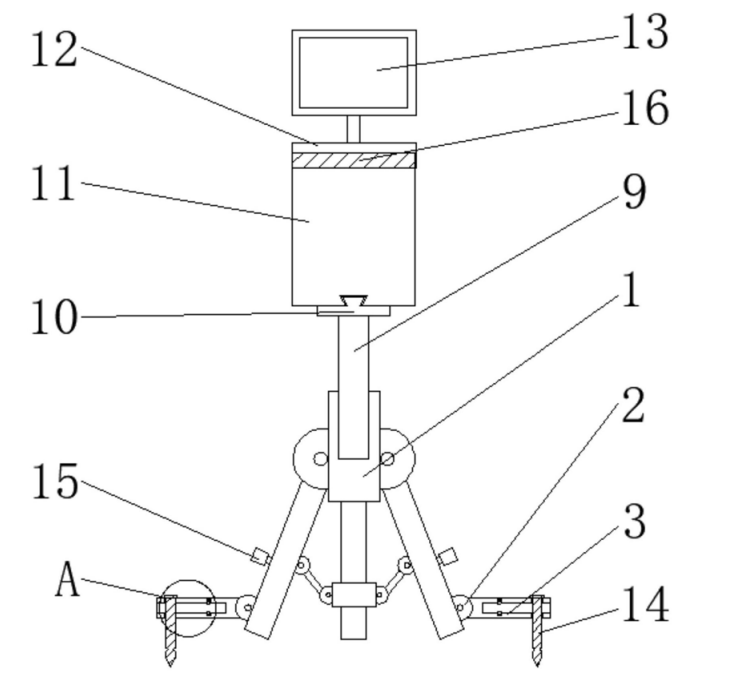
\includegraphics[width=\linewidth]{Imagenes/CN216243088U.png}
	\end{minipage}\hfill
	\begin{minipage}{0.5\textwidth}
		\centering
		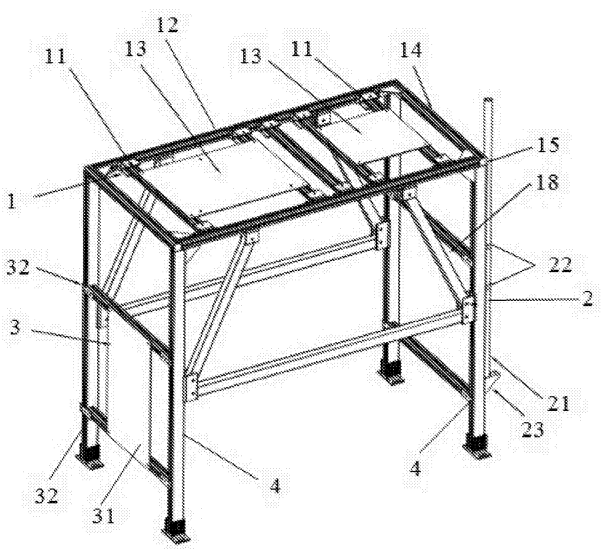
\includegraphics[width=\linewidth]{Imagenes/CN206638837U.png}
	\end{minipage}
	\par\medskip
	
	\raggedright
	\footnotesize \textit{Nota.} Adaptado de \cite{CN216243088U} (izquierda) y \cite{CN206638837U} (derecha).
	\label{fig:CN216243088U&CN206638837U}
\end{figure}

\item \textbf{Estación meteorológica simple para monitoreo ambiental (CN 206362955 U):} Se describe, como se ilustra en la Figura \ref{fig:CN206362955U&CN222047271U} (izquierda), un marco compacto (1) que integra sensores de radiación solar (7), instrumentos meteorológicos de cinco elementos para viento y otras variables (8), sensores de lluvia y sensores de temperatura, humedad y presión atmosférica mediante diversos mecanismos de fijación. Este modelo arquitectónico sirve como referencia para la distribución física del sistema de sensores a bordo de plataformas móviles, minimizando los efectos de sombreado mutuo entre instrumentos.


\item \textbf{Micro estación meteorológica automática y retractable (CN 222047271 U):} Esta patente describe, como se ilustra en la Figura \ref{fig:CN206362955U&CN222047271U} (derecha), una estación climática (2) montada sobre una base con ruedas (1) que incluye soportes roscado, compuestos por una funda roscada y una varilla roscada, y placas o almohadillas estabilizadoras (5) que se despliegan hacia abajo para anclar el equipo en superficies desniveladas. El sistema destaca por su enfoque en la estabilización mecánica del equipo de medición, utilizando estos mecanismos de anclaje desplegables que aseguran que los sensores meteorológicos mantengan un plano de referencia adecuado al evitar que la base se incline y eviten volcaduras durante la recolección de datos estáticos en terrenos con pendiente. 


\begin{figure}[H]
	
	\captionsetup{justification=raggedright, singlelinecheck=false, labelsep=none}
	
	\caption[Ilustraciones de estación meteorológica compacta y micro estación meteorológica automática con ajuste de altura.]{} 
	
	\textit{Ilustraciones de estación meteorológica compacta y micro estación meteorológica automática con ajuste de altura.} \par\medskip
	
	\begin{minipage}{0.6\textwidth}
		\centering
		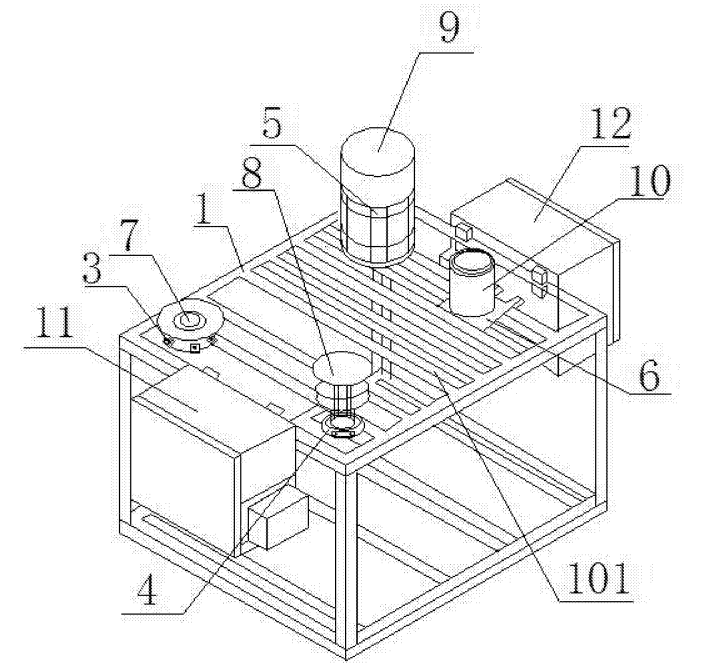
\includegraphics[width=\linewidth]{Imagenes/CN206362955U.png}
	\end{minipage}\hfill
	\begin{minipage}{0.2\textwidth}
		\centering
		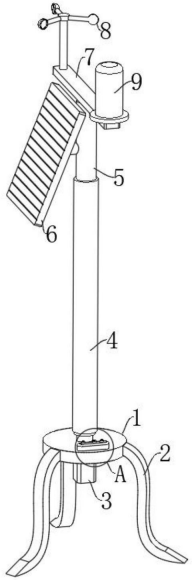
\includegraphics[width=\linewidth]{Imagenes/CN222047271U-1.png}
	\end{minipage}
	\par\medskip
	
	\raggedright
	\footnotesize \textit{Nota.} Adaptado de \cite{CN206362955U} (izquierda) y \cite{CN222047271U} (derecha).
	\label{fig:CN206362955U&CN222047271U}
\end{figure}

    \item \textbf{Instrumentación electrónica para una estación meteorológica automática (MX 2018007917 A):} Esta patente define la arquitectura de instrumentación basada en microcontroladores para el registro de variables como irradiancia global, temperatura, humedad y viento. El sistema establece la lógica de procesamiento y almacenamiento de datos en módulos locales, sirviendo de base para la programación de registro de datos embebidos.
    
    \item \textbf{MeteoPV:} Este producto comercial, visto en la Figura \ref{fig:MeteoPV} (izquierda), es una plataforma de monitorización del recurso solar diseñada específicamente para aplicaciones fotovoltaicas distribuidas. Funciona como un adquisidor de datos compacto con interfaz web integrada que facilita la configuración de piranómetros inteligentes, celdas de referencia y sensores de temperatura posterior, transmitiendo la información mediante protocolos industriales como Modbus RTU y TCP/IP hacia sistemas SCADA.
    
    	\begin{figure}[H]
    	\captionsetup{justification=raggedright, singlelinecheck=false, labelsep=none}
    	
    	\caption[Imagen de controlador MeteoPV.]{} 
    	
    	\textit{Imagen de controlador MeteoPV.} \par\medskip
    	
    	\centering
    	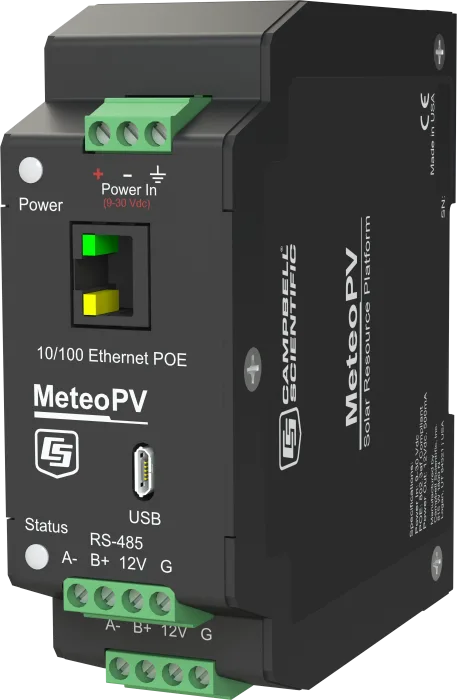
\includegraphics[width=0.3\textwidth]{Imagenes/MeteoPV.png} \par\medskip
    	
    	\raggedright
    	\footnotesize \textit{Nota.} Adaptado de \cite{MeteoPV}.
    	\label{fig:MeteoPV}
    \end{figure}
\end{itemize}

\begin{table}[H]
	\centering
	\footnotesize
	\caption{Análisis comparativo de Soluciones Parciales: Estaciones meteorológicas para plantas fotovoltaicas.}
	\label{tab:estado_arte_estaciones_pv}
	\begin{tabularx}{\textwidth}{|p{3.5cm}|>{\raggedright\arraybackslash}X|>{\raggedright\arraybackslash}X|>{\raggedright\arraybackslash}X|}
		\hline
		\rowcolor[HTML]{D9E1F2} 
		\textbf{Referente} & \textbf{Principio de Funcionamiento} & \textbf{Aporte al Proyecto} & \textbf{Limitaciones} \\ \hline
		Estación meteorológica solar multi-elemento (CN 216243088 U) & Trípode adaptativo con sistema de anclajes de bloqueo por resorte para afianzarse al suelo. & Alternativa de fijación temporal para dar rigidez al mástil de medición frente a ráfagas de viento fuertes. & Naturaleza estática; su despliegue mecánico requiere que el vehículo se detenga por completo para realizar lecturas. \\ \hline
		Sistema de monitoreo de estación meteorológica para módulos fotovoltaicos (CN 206638837 U) & Marco estructural equipado con rieles y soportes móviles que ajustan la orientación de los piranómetros. & Principio geométrico aplicable para alinear los sensores con el ángulo de inclinación de los seguidores solares. & Sistema de ajuste manual; para el UGV requerirá integración con actuadores motorizados para operación autónoma. \\ \hline
		Estación meteorológica simple para monitoreo ambiental (CN 206362955 U) & Estructura estática compacta que integra en un solo marco sensores de radiación, viento, lluvia y temperatura. & Referencia para la distribución física de la suite de sensores a bordo de plataformas móviles, minimizando sombreados. & Diseño estático fijo que no permite la adaptación dinámica al ángulo de incidencia solar. \\ \hline
		Instrumentación electrónica para una estación meteorológica automática (MX 2018007917 A) & Arquitectura basada en microcontroladores para el registro de variables climáticas en módulos locales SD. & Establece la lógica de procesamiento y almacenamiento de datos para registradores de datos embebidos. & Sistema básico de registro sin capacidades de telemetría de largo alcance integradas. \\ \hline
		Micro estación meteorológica automática y retractable (CN 222047271 U) & Mástil de medición basado en un tubo telescópico extendido verticalmente por un motor eléctrico. & Permite elevar instrumentos para evadir las turbulencias y el polvo generado por el chasis móvil. & Elevar el mástil modifica el centro de gravedad del robot, lo que podría desestabilizarlo al transitar sobre pendientes. \\ \hline
		Plataforma MeteoPV & Datalogger comercial que concentra datos de sensores inteligentes y los transmite mediante Modbus RTU/TCP. & Prototipo comercial directo para la arquitectura de adquisición del UGV; asegura inmunidad ante el ruido de los motores. & Es un módulo pasivo diseñado para montaje estandarizado; requiere gestión de disipación térmica y no controla locomoción. \\ \hline
	\end{tabularx}
\end{table}
\subsubsection{Ajuste de orientación para sensores de irradiancia}

\begin{itemize}
	
	
    \item \textbf{Seguidor solar SOLYS2} Este producto, visto en la Figura \ref{fig:ZippZonen_Tracker&Radiometer} (derecha) es un seguidor solar de alta precisión que incluye un receptor GPS integrado para la configuración automática de las coordenadas geográficas y la hora. Su diseño permite un seguimiento exacto para orientar instrumentos de medición directa, eliminando la necesidad de ajustes manuales constantes o sincronización por computadora externa.
	
    
    \item \textbf{Kit de montaje para piranómetro con inclinación ajustable} Este producto, visto en la Figura \ref{fig:ZippZonen_Tracker&Radiometer}, trata de un soporte mecánico con escala graduada diseñado para montar piranómetros en ángulos de inclinación específicos de $0^{\circ}$ a $90^{\circ}$. Este kit permite igualar manualmente la inclinación de los sensores con la de los paneles fotovoltaicos fijos, asegurando que la irradiancia medida sea la misma que incide sobre la superficie de generación.
    
    
    \begin{figure}[H]
    	
    	\captionsetup{justification=raggedright, singlelinecheck=false, labelsep=none}
    	
    	\caption[Kit de montaje para piranómetro con inclinación ajustable de KIPP \& ZONEN.]{} 
    	
    	\textit{Fotos de módulo controlador MeteoPV y seguidor solar SOLYS2 de KIPP \& ZONEN.} \par\medskip
    	
    	\begin{minipage}{0.5\textwidth}
    		\centering
    		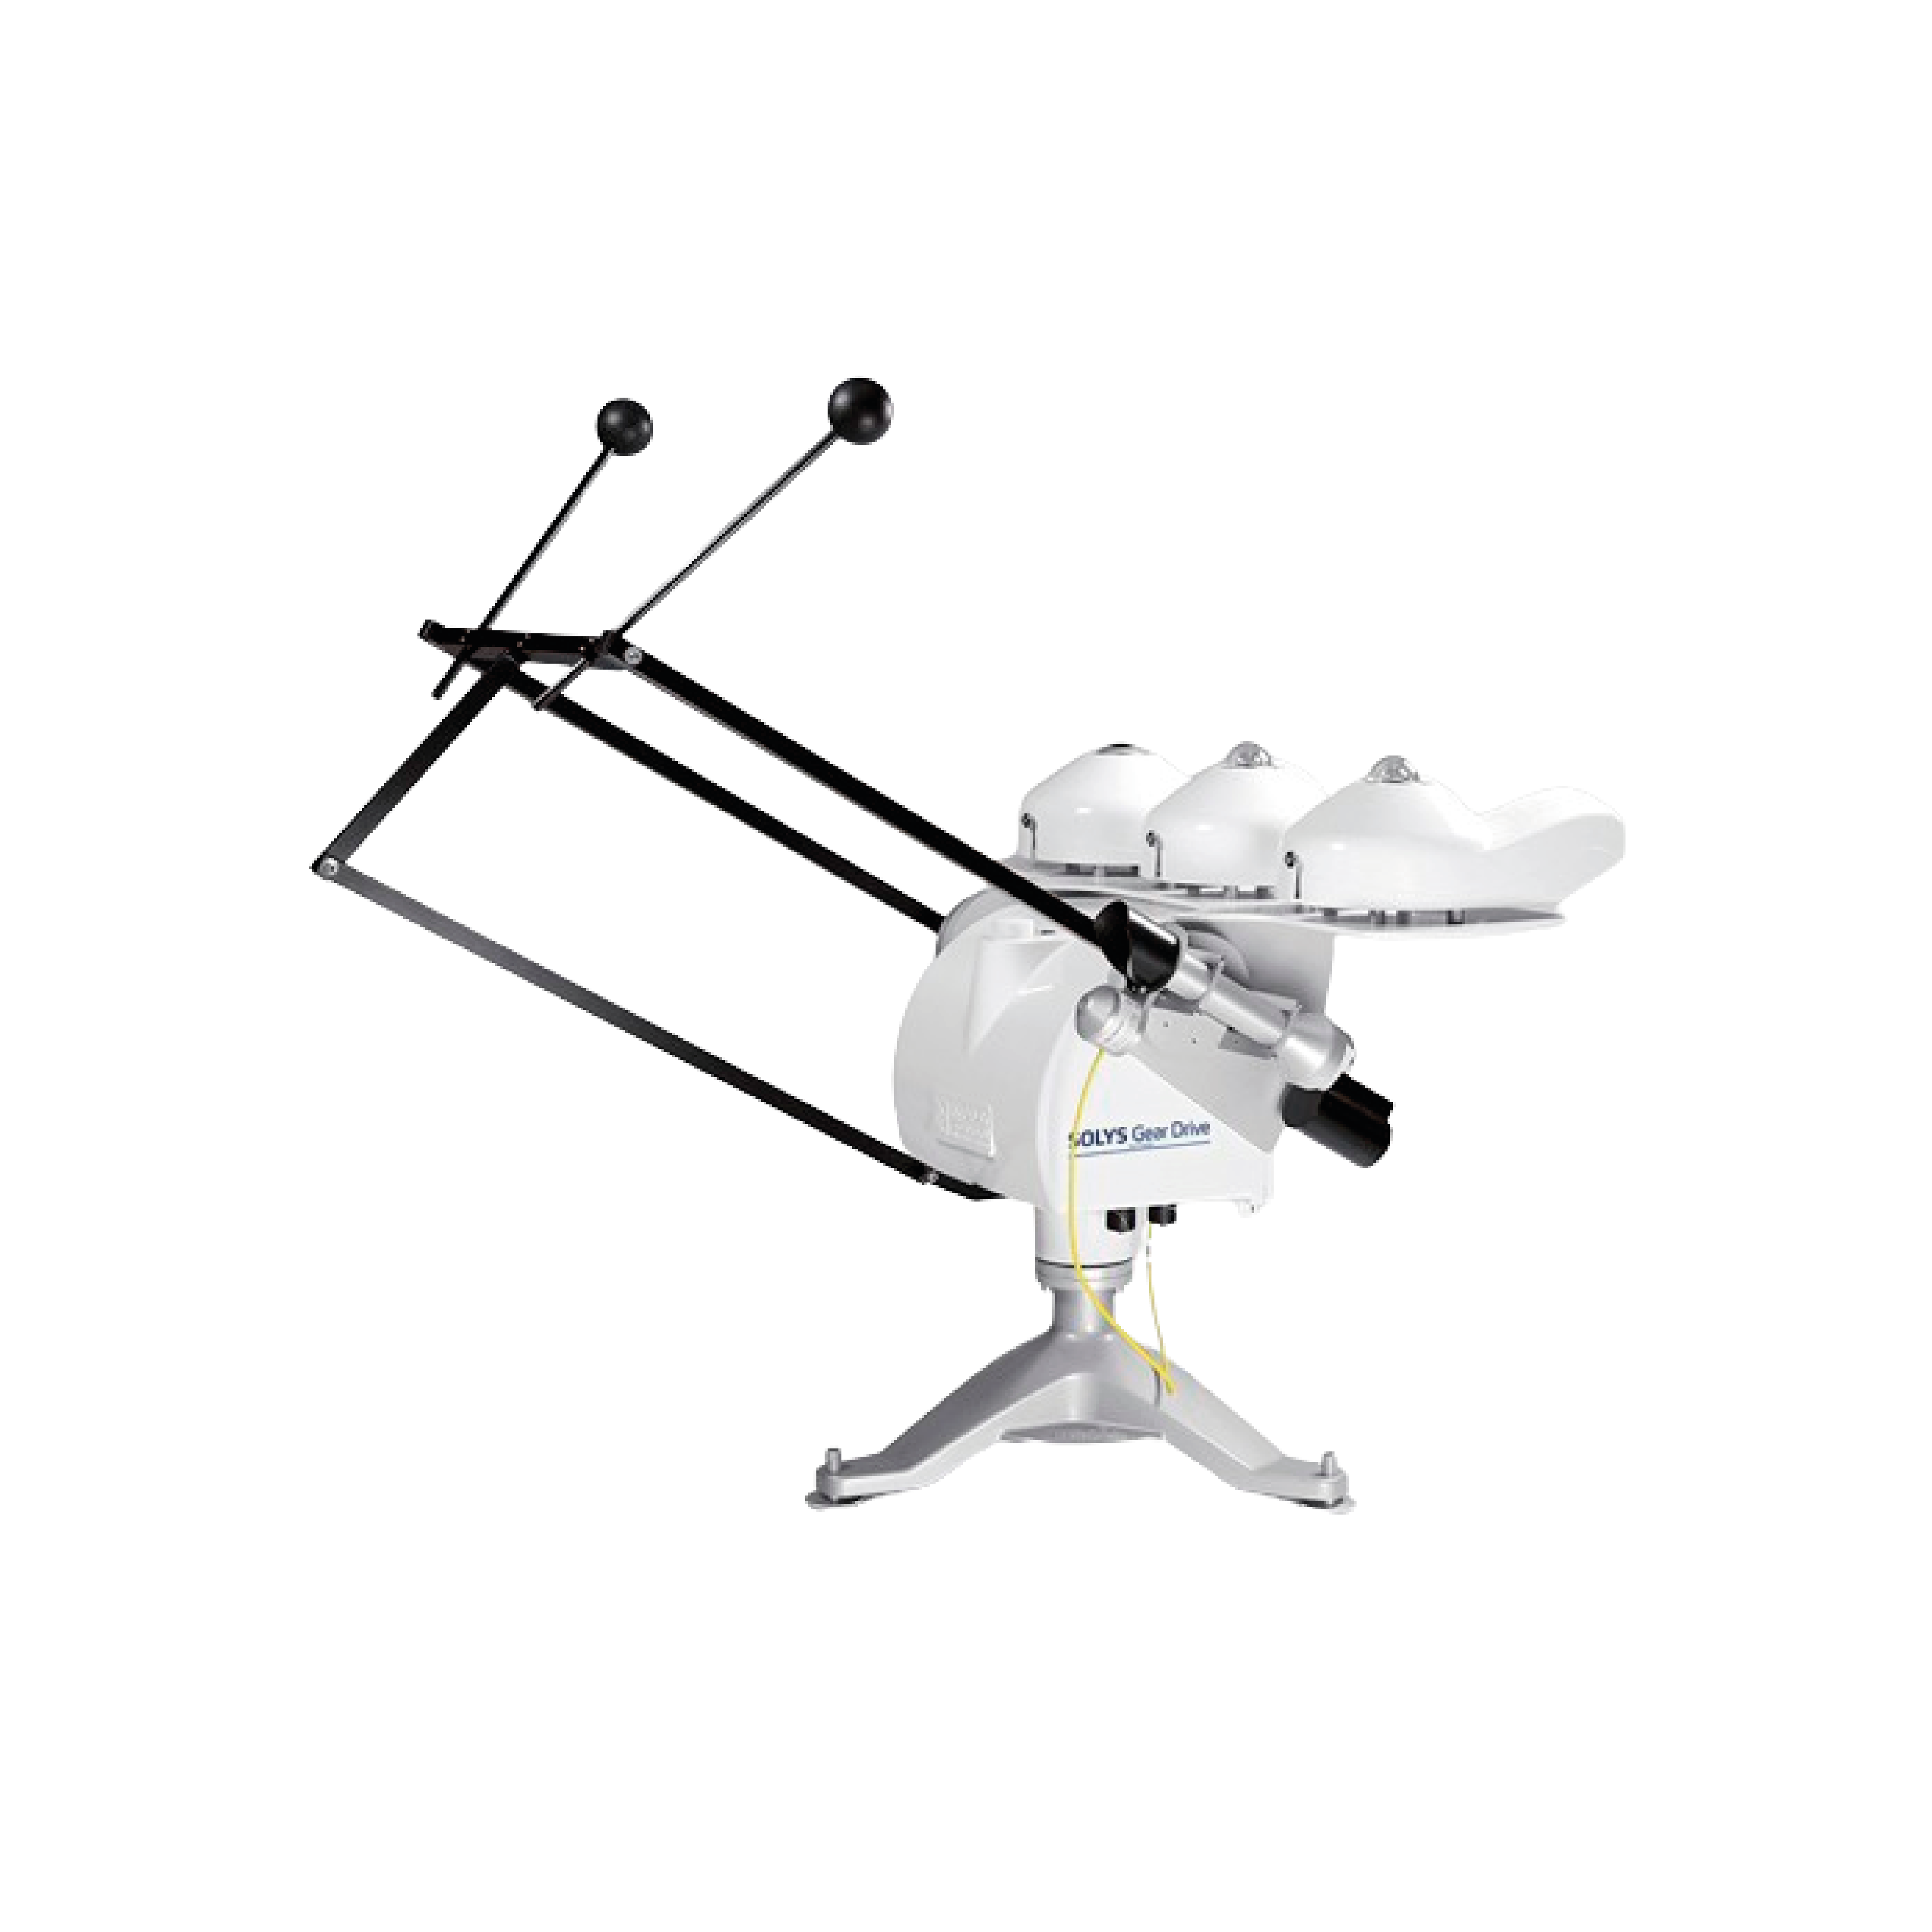
\includegraphics[width=\linewidth]{Imagenes/KippZonen_SunTrackers.png}
    	\end{minipage}\hfill
    	\begin{minipage}{0.5\textwidth}
    		\centering
    		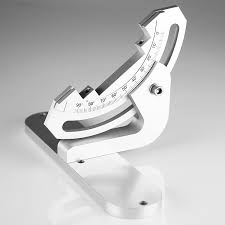
\includegraphics[width=\linewidth]{Imagenes/KippZonen_Radiometer.jpg}
    	\end{minipage}
    	\par\medskip
    	
    	\raggedright
    	\footnotesize \textit{Nota.} Adaptado de \cite{KippZonen_SunTrackers} (izquierda) y \cite{KippZonen_Radiometer} (derecha).
    	\label{fig:ZippZonen_Tracker&Radiometer}
    \end{figure}
    
    
\end{itemize}

\begin{table}[H]
	\centering
	\footnotesize
	\caption{Análisis comparativo de Soluciones Parciales: Sistemas de comunicación para datos meteorológicos.}
	\label{tab:estado_arte_comunicacion}
	\begin{tabularx}{\textwidth}{|p{3.5cm}|>{\raggedright\arraybackslash}X|>{\raggedright\arraybackslash}X|>{\raggedright\arraybackslash}X|}
		\hline
		\rowcolor[HTML]{D9E1F2} 
		\textbf{Referente} & \textbf{Principio de Funcionamiento} & \textbf{Aporte al Proyecto} & \textbf{Limitaciones} \\ \hline
		Estación meteorológica avanzada IoT (SK 302020 A3) & Sistema meteorológico IoT con un avanzado bloque de gestión y recuperación de baterías (BMS). & Permite administrar la energía de los sensores de forma independiente a otros sistemas motrices del vehículo. & No aborda aspectos de navegación o estabilidad mecánica requeridos para la movilidad en planta. \\ \hline
		Sistema de monitoreo de plantación basado en LoRa (CN 208458788 U) & Utiliza nodos sensores móviles y fijos conectados mediante red inalámbrica LoRa a un gateway central. & Permite la transmisión de datos a largas distancias con bajo consumo, ideal para supervisión remota en plantas extensas. & La latencia inherente a LoRa puede limitar la frecuencia de muestreo en inspecciones de alta velocidad. \\ \hline
		Método de posicionamiento para robots móviles (CN 116405876 A) & Emplea módulos LoRa para comunicación y cálculo de ubicación mediante intensidad de señal y tiempo de llegada. & Proporciona un método de localización en tiempo real para el seguimiento preciso de la ruta del vehículo. & Requiere la instalación de múltiples gateways distribuidos en el área operativa para garantizar precisión. \\ \hline
	\end{tabularx}
\end{table}


\subsubsection{Sistemas de comunicación para datos meteorológicos}
\begin{itemize}
    \item \textbf{Estación meteorológica avanzada IoT (SK 302020 A3):} Esta solución detalla un sistema meteorológico dividido en bloques funcionales, donde resalta un bloque avanzado de gestión y recuperación de baterías. Este esquema permite administrar la energía de los sensores de forma independiente a otros sistemas motrices, garantizando la continuidad de la toma de datos IoT incluso en condiciones de baja carga.
    
    \item \textbf{Sistema de monitoreo de plantación basado en LoRa (CN 208458788 U):} Este sistema utiliza la tecnología de comunicación inalámbrica LoRa para conectar múltiples nodos sensores, tanto móviles como fijos, con un gateway central. La arquitectura permite transmitir datos ambientales de irradiancia, viento y temperatura a largas distancias con bajo consumo energético, facilitando la supervisión remota a través de plataformas en la nube.
    
    \item \textbf{Método de posicionamiento para robots móviles (CN 116405876 A):} El método emplea módulos LoRa instalados en robots móviles que se comunican con gateways fijos distribuidos en el área de operación. Mediante el análisis de la intensidad de señal y el tiempo de llegada, el sistema permite determinar la ubicación precisa del vehículo en tiempo real y transmitir sus datos operativos hacia un servidor de control.
\end{itemize}

%

\begin{table}[H]
	\centering
	\footnotesize
	\caption{Análisis comparativo de Soluciones Parciales: Ajuste de orientación para sensores de irradiancia.}
	\label{tab:estado_arte_ajuste_sensores}
	\begin{tabularx}{\textwidth}{|p{3.5cm}|>{\raggedright\arraybackslash}X|>{\raggedright\arraybackslash}X|>{\raggedright\arraybackslash}X|}
		\hline
		\rowcolor[HTML]{D9E1F2} 
		\textbf{Referente} & \textbf{Principio de Funcionamiento} & \textbf{Aporte al Proyecto} & \textbf{Limitaciones} \\ \hline
		Seguidor solar SOLYS2 & Seguidor solar automático con receptor GPS integrado para configuración autónoma de ubicación y tiempo. & Referencia para el seguimiento exacto de la trayectoria solar para instrumentos de medición directa. & Elevado peso y costo para ser integrado en una plataforma móvil de exploración dinámica. \\ \hline
		Kit de montaje para piranómetro con inclinación ajustable & Soporte mecánico con escala graduada para montaje de piranómetros en ángulos de $0^{\circ}$ a $90^{\circ}$. & Permite igualar manualmente la inclinación de los sensores con la de los paneles fotovoltaicos fijos (Plano POA). & Requiere intervención humana para el ajuste del ángulo de inclinación inicial. \\ \hline
	\end{tabularx}
\end{table}
%
%
\section{Identificación de usuarios}

El diseño y la implementación del robot autónomo para la medición de variables climáticas involucra a diversos actores dentro del ecosistema de una planta solar fotovoltaica a gran escala. Identificar a estos usuarios y comprender sus necesidades específicas es fundamental para establecer los requerimientos de diseño del sistema mecatrónico. Los agentes involucrados se clasifican en usuarios directos e indirectos.

Para estructurar visualmente el nivel de interacción de cada actor con el equipo y sus datos, se emplea un Stakeholder Map basado en un modelo concéntrico (ver \ref{fig:StakeholderMap}). Esta herramienta clasifica a los agentes en tres niveles de proximidad: el núcleo operativo, el entorno comercial y de gestión y la periferia normativa e institucional.

    	\begin{figure}[H]
	\captionsetup{justification=raggedright, singlelinecheck=false, labelsep=none}
	
	\caption[Stakeholder Map con usuario principal, usuarios directos e indirectos]{} 
	
	\textit{Stakeholder Map con usuario principal, usuarios directos e indirectos} \par\medskip
	
	\centering
	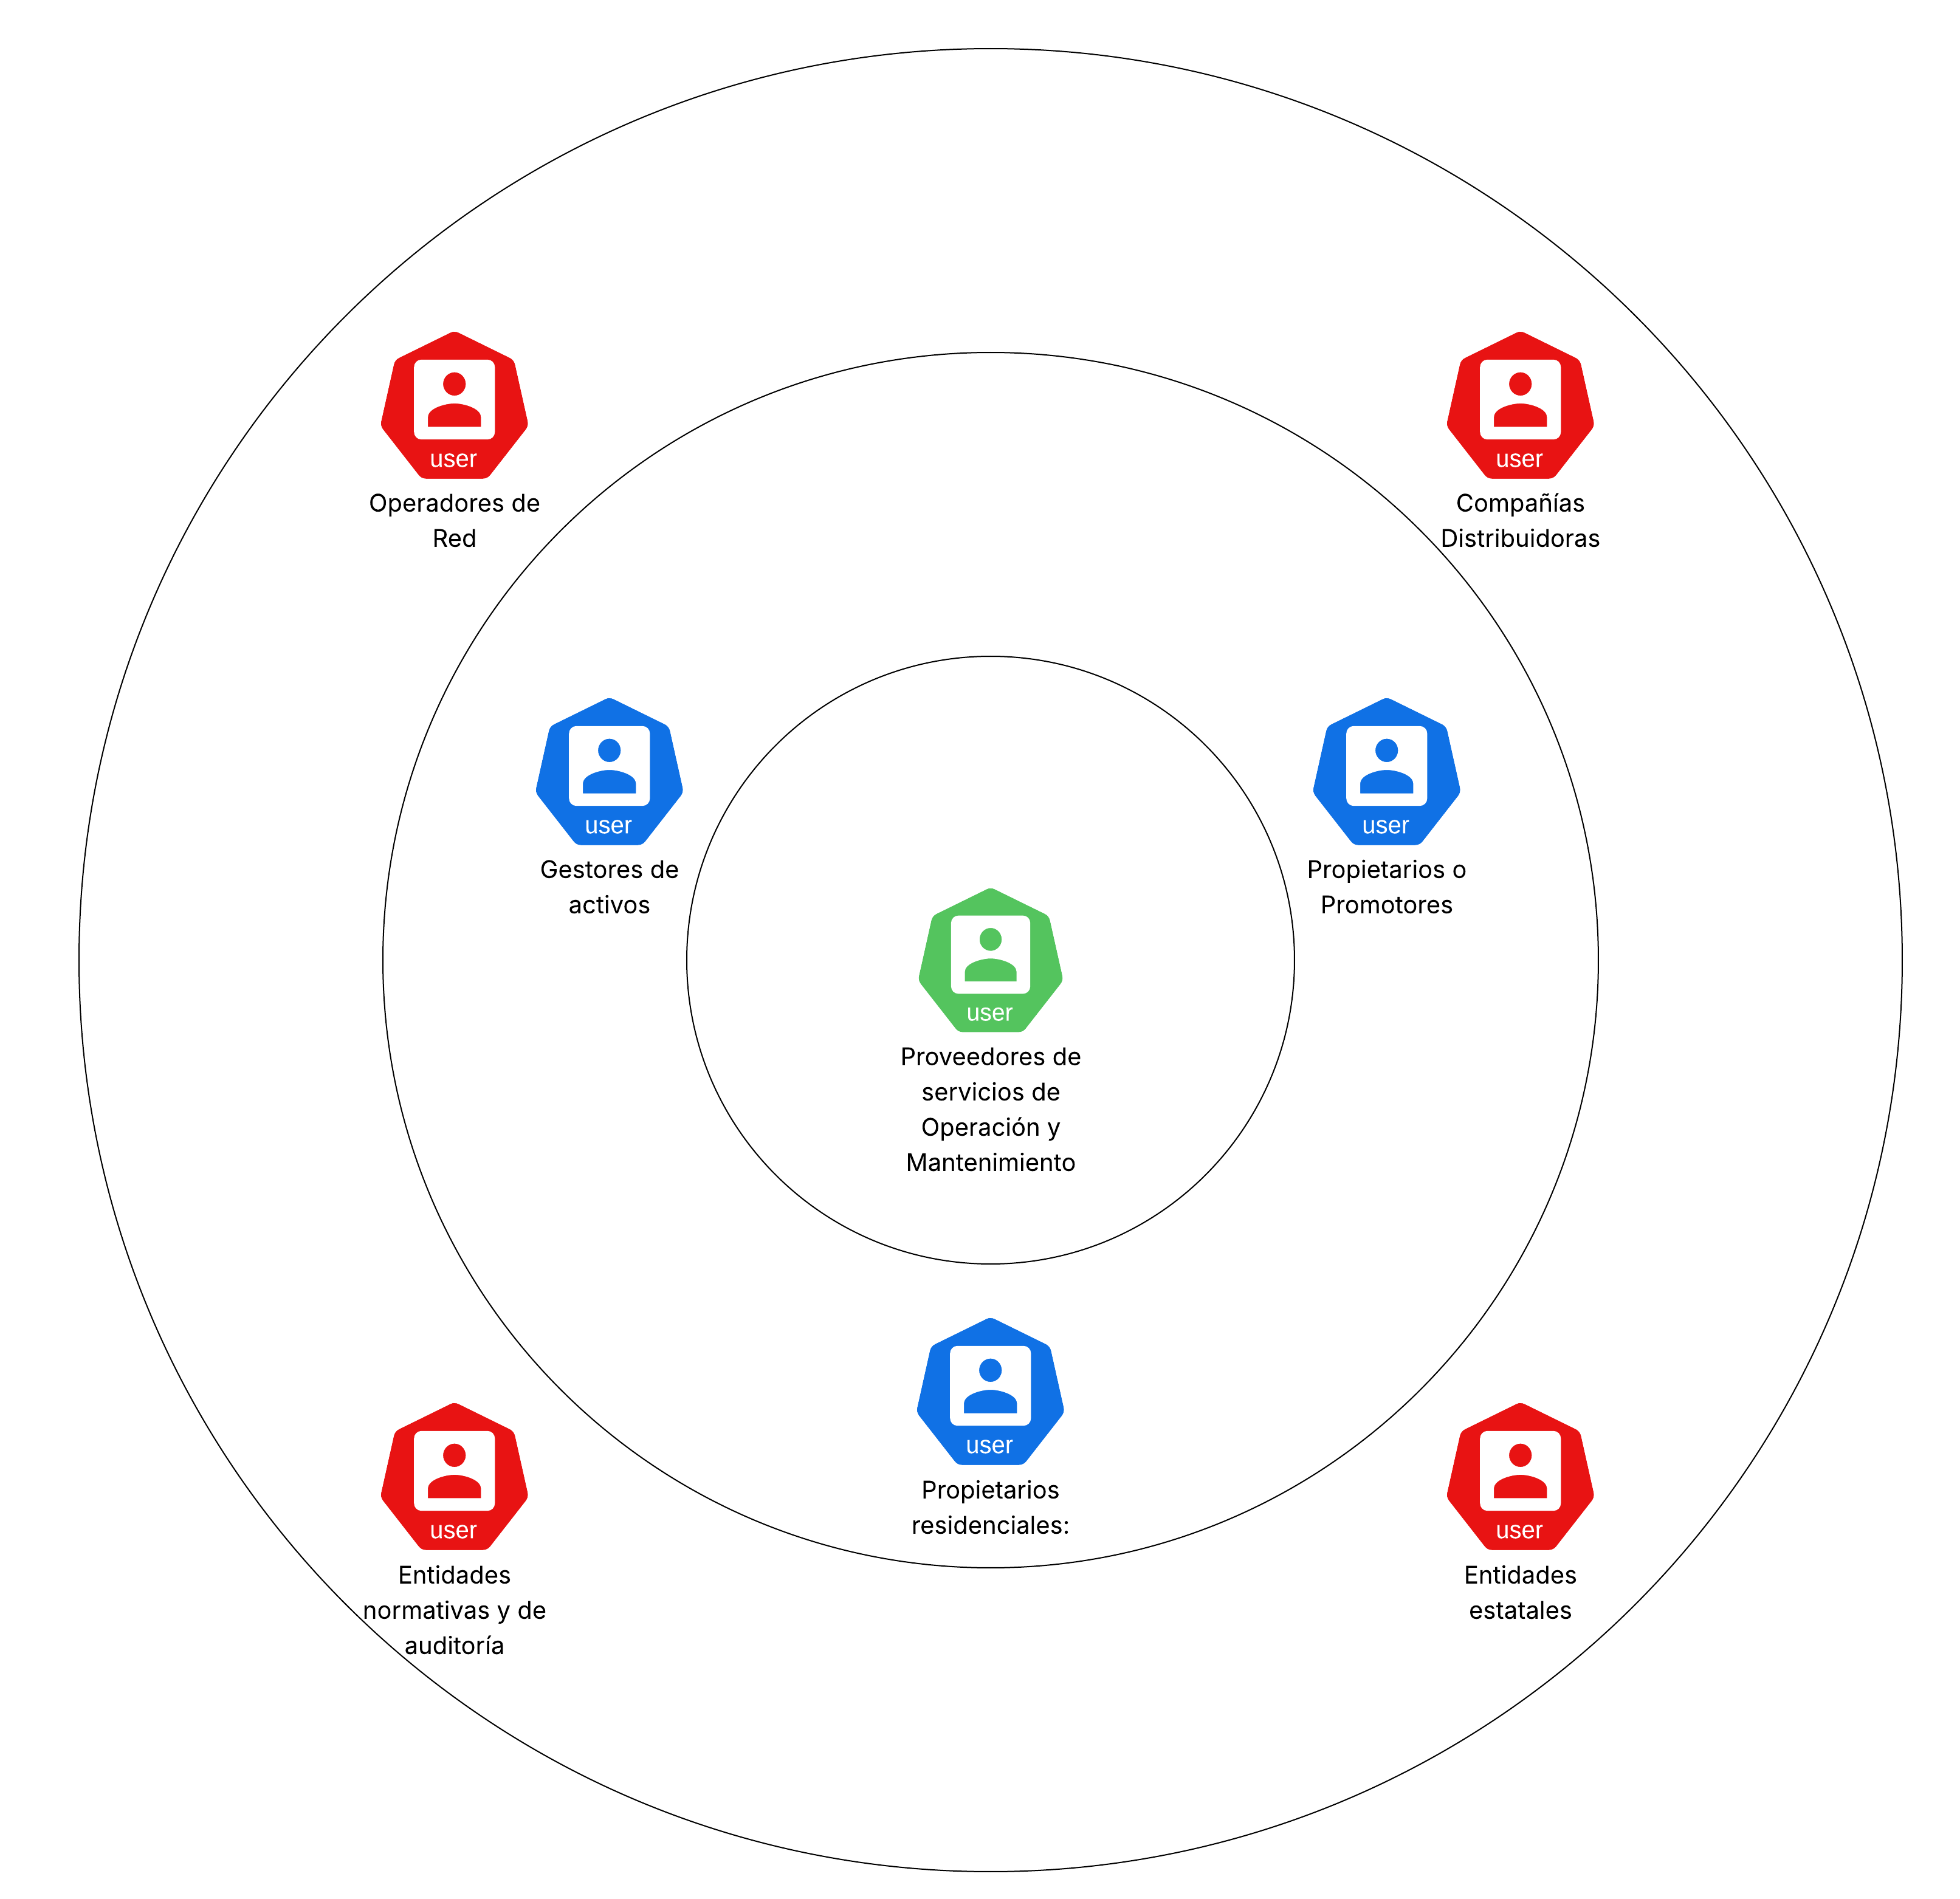
\includegraphics[width=\textwidth]{Imagenes/StakeholderMap.png} \par\medskip
	
	\raggedright
	\footnotesize \textit{Nota.} Elaboración propia.
	\label{fig:StakeholderMap}
\end{figure}

\subsection{Usuario principal}

El usuario principal es aquel cuyas necesidades sirven como base principal de los requerimientos del proyecto.
\begin{itemize}
	
	
 \item \textbf{Proveedores de servicios de Operación y Mantenimiento (O\&M):} Personal técnico y de ingeniería encargado del funcionamiento diario de la planta. Su necesidad principal es transicionar de un enfoque de mantenimiento correctivo a uno predictivo y preventivo. Además, necesitan capturar datos climáticos precisos para cuantificar objetivamente las pérdidas por ensuciamiento y optimizar así sus ciclos de limpieza \citep{TesisJGB}.
\end{itemize}

\subsection{Usuarios directos}
Estos usuarios interactúan directamente con los datos generados por el sistema o dependen de ellos para la gestión técnica y comercial de la planta:

\begin{itemize}

    
    \item \textbf{Gestores de activos}: Profesionales o entidades responsables de la gestión comercial y financiera de la inversión en energía renovable, así como de la supervisión y control de las actividades técnicas delegadas a los contratistas de O\&M. Para llevar a cabo su labor de auditoría, requieren que la recolección de datos capture la variabilidad climática adecuada en el terreno. Esto les permite evaluar la salud de los activos, calcular con exactitud los indicadores clave de rendimiento, y comparar de forma objetiva si el rendimiento energético medido en el parque cumple con las expectativas de diseño \citep{ProyectoEjecutivo2024}.
    
    \item \textbf{Propietarios o Promotores}: Entidades inversoras o corporaciones dueñas de la instalación fotovoltaica que financian y promueven el proyecto desde su concepción. Su necesidad principal es salvaguardar la viabilidad del proyecto a largo plazo, reducir costos y prolongar la vida útil de los equipos para maximizar la rentabilidad de la infraestructura. Para ellos, disponer de mediciones climáticas dinámicas y representativas se traduce en una reducción de la incertidumbre operativa y financiera, garantizando que el retorno de inversión esté respaldado por datos confiables sobre el recurso solar\citep{ProyectoEjecutivo2024}.
    
    \item \textbf{Propietarios residenciales (Personas naturales)}: : Representan a los individuos que poseen plantas fotovoltaicas personales, ya sean sistemas de generación distribuida orientados al autoconsumo o sistemas \textit{off-grid}. Aunque estas instalaciones operan a una escala mucho menor enfocada en la microgeneración, estos usuarios comparten la necesidad de contar con sistemas de medición accesibles que les permitan contrastar las variables climáticas locales con la producción de sus módulos. 
\end{itemize}

\subsection{Agentes indirectos}
Estos actores imponen las condiciones y los estándares de calidad bajo los cuales los datos del robot deben ser recolectados y transmitidos:

\begin{itemize}

    \item \textbf{Operadores de Red:} Entidades encargadas de la gestión de la red eléctrica nacional o regional. Necesitan que la planta fotovoltaica garantice una inyección de potencia predecible. La recolección dinámica de datos climáticos ayuda a prever fluctuaciones en la generación, permitiendo que los sistemas de control regulen adecuadamente la potencia activa y reactiva en el punto de interconexión (Kenemora Solar, 2024).
    
    \item \textbf{Compañías Distribuidoras:} Entidades encargadas de la facturación, los contratos y atención al cliente tanto a pequeña como mediana escala. Su principal interés es conocer al detalle el costo de la energía eléctrica para poder generar contratos mutuamente beneficiosos para ambas partes. En este sentido, las fluctuaciones en la generación ocasionan fuertes cambios en el costo de la energía, a veces sin posibilidad de modificar el costo que paga el cliente.
    
    \item \textbf{Entidades estatales (COES):} El Comité de Operación Económica del Sistema (COES) tiene la misión de planificar la generación de cada una de las plantas, y asegurarse de que no haya un desbalance entre la energía generada y consumida por la ciudad. Para cumplir con este objetivo, requiere predicciones precisas de parte de las plantas renovables en la producción, para poder ordenar con precisión a las plantas no renovables los rangos de potencia a producir.
    
    \item \textbf{Entidades normativas y de auditoría técnica:} Organismos internacionales e independientes que establecen los estándares de calidad. Imponen la necesidad de que los datos recolectados posean trazabilidad, exactitud comprobable e instrumentación validada, de modo que los diagnósticos y las pruebas de evaluación de capacidad de la planta tengan total validez legal frente a terceros. Esto obliga a que el sistema se adhiera rigurosamente a estándares internacionales como la norma IEC 61724-1 para la monitorización general, y la IEC TS 61724-2 para los métodos de evaluación de capacidad.

\end{itemize}

% 
%
\section{Lista de requerimientos}
A continuación, se presenta la lista de requerimientos del sistema, la cual traduce las necesidades identificadas de los stakeholders en parámetros técnicos cuantificables. Esta tabla funciona como el contrato técnico del proyecto y clasifica las especificaciones en exigencias (E) y deseos (D), agrupándolas según las características establecidas por la metodología.
%
%
%
%
%
\begin{center}
\footnotesize
\begin{xltabular}{\textwidth}{|p{0.6cm}|c|p{2.2cm}|>{\raggedright\arraybackslash}X|>{\raggedright\arraybackslash}X|>{\raggedright\arraybackslash}X|}
\caption{Lista de requerimientos del sistema mecatrónico.}
\label{tab:lista_requerimientos} \\
\hline
\rowcolor[HTML]{D9E1F2} 
\textbf{ID} & \textbf{Tipo} & \textbf{Característica} & \textbf{Descripción técnica} & \textbf{Fuente / Justificación} & \textbf{Método de verificación} \\ \hline
\endfirsthead

\multicolumn{6}{c}%
{{\bfseries Continuación de la \tablename\ \thetable{}}} \\
\hline
\rowcolor[HTML]{D9E1F2} 
\textbf{ID} & \textbf{Tipo} & \textbf{Característica} & \textbf{Descripción técnica} & \textbf{Fuente / Justificación} & \textbf{Método de verificación} \\ \hline
\endhead

\hline
\endfoot

\hline
\endlastfoot

1 & E & Geometría & El vehículo debe tener dimensiones máximas de 600x600x500 mm y una masa total inferior a 20kg. & Restricciones espaciales de los pasillos entre los seguidores solares y límites ergonómicos de carga para los operarios  \citep{ProyectoEjecutivo2024}. & Inspección con cinta métrica y pesaje con balanza industrial calibrada. \\ \hline
2 & E & Cinemática & El robot debe desplazarse por los pasillos de la planta a una velocidad nominal de 1 m/s. & Necesidad de cubrir el área de inspección en un tiempo razonable sin comprometer la estabilidad de los sensores  \citep{ProyectoEjecutivo2024}. & Prueba de cinemática midiendo el tiempo de recorrido en un circuito de longitud conocida. \\ \hline
3 & E & Fuerzas / Cinemática & El sistema de locomoción debe ser capaz de superar pendientes con una inclinación de hasta 14°. & Topografía irregular, zanjas erosivas y desniveles comunes en las plantas solares a gran escala \citep{Salinas2025}. & Ensayo de tracción y estabilidad en rampa de prueba con inclinación ajustable. \\ \hline

4 & E & \multirow{2.5}{*}{Energía} & El sistema de almacenamiento y suministro de energía debe proporcionar una autonomía de operación ininterrumpida de al menos 1 hora sin requerir recarga externa. & El robot debe completar ciclos de inspección completos antes de verse forzado a recargar en una estación base \citep{ProyectoEjecutivo2024}. & Ensayo de descarga de energía bajo consumo nominal de motores e instrumentación. \\ \hline
5 & E & Materia / Fuerzas & La envolvente del vehículo y los gabinetes de la electrónica deben cumplir con un grado de protección IP44 e IK08. & Exposición severa a polvo del desierto, lluvias eventuales y posibles impactos mecánicos durante el recorrido \citep{ProyectoEjecutivo2024}. & Revisión de la certificación de los gabinetes y prueba de hermeticidad con chorro de agua. \\ \hline
6 & E & Materia & El sistema mecatrónico debe operar sin degradación en un rango de temperatura ambiente de 10°C a 30°C. & Las plantas fotovoltaicas suelen emplazarse en zonas áridas con altas oscilaciones térmicas \citep{Salinas2025}. & Ensayo de estrés térmico de los componentes críticos en cámara climática. \\ \hline
7 & E & \multirow{4}{*}{Señales} & El instrumento de medición de irradiancia a bordo debe contar con una exactitud de Clase A bajo el estándar internacional aplicable. & Requisito normativo estricto para garantizar que el cálculo del \textit{Performance Ratio} tenga una baja incertidumbre \citep{IEC61724-1_2021}. & Verificación del \textit{datasheet} comercial y del certificado de calibración del instrumento. \\ \cline{1-2} \cline{4-6}
8 & E & & El sistema de adquisición debe muestrear las variables meteorológicas en un intervalo de 5 segundos y registrarlas con una frecuencia máxima de 5 minutos. & Recomendaciones para el monitoreo meteorológico de precisión para capturar ráfagas o eventos rápidos de sombreado \citep{IEC61724-1_2021}. & Análisis de las marcas de tiempo en los archivos de almacenamiento de datos. \\ \hline
9 & E & Control & El sistema de navegación debe detectar obstáculos imprevistos dentro del área de un semicírculo de 1 metro de radio, ubicado en cada dirección de movimiento del robot, y recalcular su trayectoria para evadirlos. & Presencia de rocas, vegetación crecida o personal de mantenimiento bloqueando temporalmente el pasillo \citep{Figgis2025}. & Prueba de campo colocando obstáculos ciegos en la ruta predefinida del robot. \\ \hline
10 & E & Comunicación & El módulo de telemetría debe transmitir los paquetes de datos a la estación base garantizando un alcance efectivo mínimo de 200 metros en línea de vista. & Las plantas solares a escala comercial abarcan grandes extensiones de terreno longitudinal \citep{Figgis2025}. & Ensayo de pérdida de paquetes (\textit{ping}) alejando el robot progresivamente de la estación base. \\ \hline

11 & D & Mantenimiento & El robot debe incorporar un mecanismo o actuador capaz de mitigar la acumulación de suciedad en los sensores con una efectividad de limpieza que mantenga una incertidumbre menor al 2\%. & La suciedad acumulada degrada críticamente la exactitud de los instrumentos de medición de irradiancia \citep{IEC61724-1_2021}. & Medición comparativa de irradiancia antes y después de activar el mecanismo bajo suciedad simulada. \\ \hline
12 & E & Seguridad & El vehículo debe disponer de un sistema de parada de emergencia que interrumpa la tracción en un tiempo de respuesta menor a 0.1 segundos. & Prevención de accidentes industriales y protección frente a pérdida total de control en la navegación \citep{ProyectoEjecutivo2024}. & Prueba de interrupción forzada de marcha cronometrada en laboratorio. \\ \hline

\end{xltabular}
\end{center}





%----------------------------------------------------------------------------------------
%	Capítulo 3
%----------------------------------------------------------------------------------------

%{TFC1/cap3}
\onehalfspacing
\fancypagestyle{plain}{
	\fancyhf{}
	\rhead{\thepage}
	\renewcommand{\headrulewidth}{0pt}
	\renewcommand{\footrulewidth}{0pt}
}

\chapter{DISEÑO CONCEPTUAL}

\section{Caja Negra}

Como primer paso para el modelado del diseño conceptual, es fundamental delimitar las fronteras del proyecto y comprender los elementos del sistema fotovoltaico con los que este va a interactuar. Para ello, se emplea el diagrama de Black Box, el cual permite visualizar la operación del sistema en su nivel más alto de abstracción mediante la representación de sus entradas y salidas.

En la Figura \ref{fig:caja_negra} se presenta la abstracción funcional del sistema de inspección a nivel de caja negra, la cual define las fronteras del producto y su interacción con el entorno.

\begin{figure}[H]
	\captionsetup{justification=raggedright, singlelinecheck=false, labelsep=none}
	\caption[Abstracción funcional del sistema de inspección a nivel de caja negra.]{} 
	\textit{Abstracción funcional del sistema de inspección a nivel de caja negra.} \par\medskip
	
	\makebox[\textwidth][c]{ 
		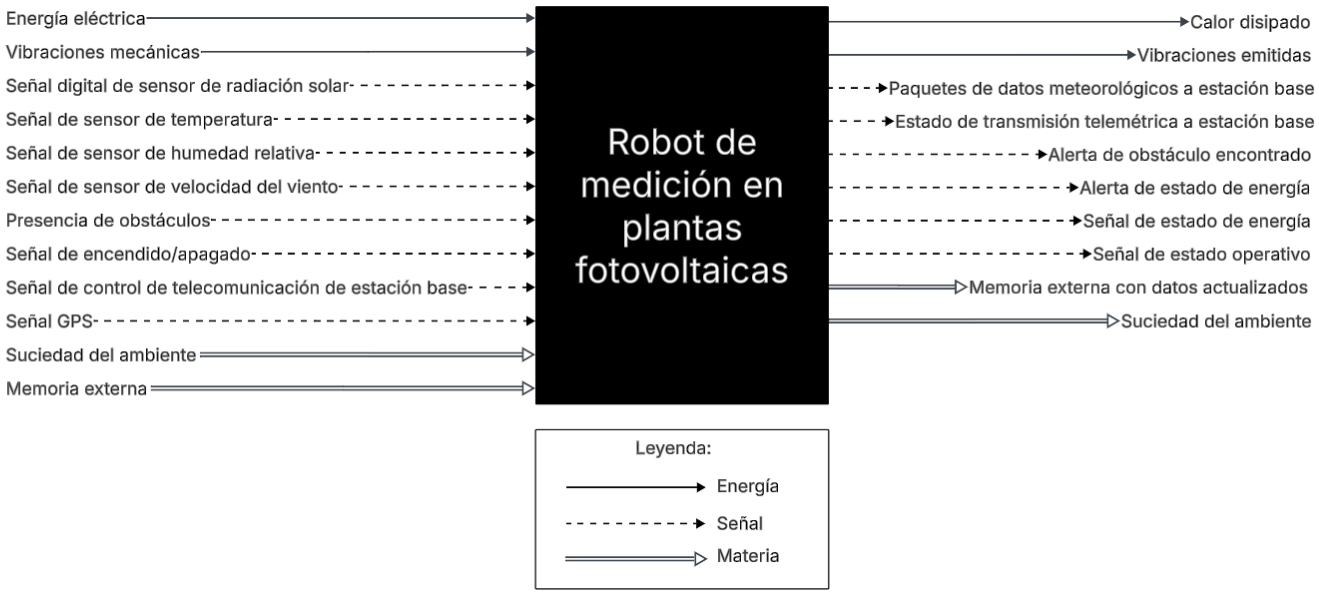
\includegraphics[width=1.2\textwidth]{Imagenes/A3_Blackbox_v7.png}
	} \par\medskip
	
	\raggedright
	\footnotesize \textit{Nota.} Elaboración propia.
	\label{fig:caja_negra}
\end{figure}

La función principal del sistema se define como: Transformar señales de instrumentación meteorológica externa, información espacial y comandos del usuario en paquetes de datos procesados con validez industrial y reportes de estado telemétrico.

Para cumplir con su objetivo, el sistema recibe flujos de energía de entrada compuestos por la energía eléctrica directa necesaria para su alimentación y las perturbaciones provenientes del terreno en forma de vibraciones mecánicas.

Simultáneamente, el sistema capta flujos de señales e información provenientes del entorno, las cuales incluyen la data climática (señal digital de sensor de radiación solar, señal de sensor de temperatura, señal de sensor de humedad relativa y señal de sensor de velocidad del viento), la señal GPS y la presencia de obstáculos; mientras que, desde el exterior, se introducen las instrucciones mediante la señal de encendido/apagado y la señal de control de telecomunicación de estación base.

Por otro lado, los flujos de materia que interactúan en las fronteras de entrada del sistema corresponden a la inserción física de la memoria externa y al ingreso inevitable de la suciedad del ambiente, propia de las instalaciones fotovoltaicas.

Como resultado de la transformación interna, el sistema entrega, como salidas útiles, un flujo de información compuesto por los paquetes de datos meteorológicos a estación base, el estado de transmisión telemétrica a estación base, las advertencias críticas de alerta de obstáculo encontrado y alerta de estado de energía, así como la señal de estado de energía y la señal de estado operativo requeridas para la interfaz local. Es importante destacar que estos flujos de comunicación, tanto de entrada como de salida, representan tramas de bytes estructuradas, garantizando la integridad y correcta interpretación de la telemetría.

A nivel de flujos de materia, el sistema depara la extracción de la memoria externa con datos actualizados, la cual contiene el respaldo físico de la información, y la evacuación o paso de la suciedad del ambiente.

Finalmente, como residuo del trabajo físico y computacional, el sistema libera al entorno flujos de energía en forma de calor disipado y vibraciones emitidas durante su desplazamiento continuo. Además, el sistema provee como salida un flujo de energía eléctrica para sensores meteorológicos, asegurando la alimentación y operatividad de la instrumentación externa.


\section{Estructura de Funciones}

A partir de la caja negra, se desarrolla la estructura de funciones (ver Anexo 2). En este esquema, la función principal del sistema se descompone en dominios, cada uno con bloques que describen las funciones elementales del robot, relacionando detalladamente los flujos internos de energía, materia y señales.

\subsection{Dominio de Energía}
El Dominio de Energía se encarga de la recepción, gestión y distribución del recurso eléctrico necesario para garantizar el funcionamiento de todos los subsistemas del robot, a través del siguiente flujo, ilustrado en la Figura \ref{Avance3_DomEnergia}:

\begin{itemize}
	\item \textbf{Recibir energía eléctrica:} Para esta función se evaluó el conector \textit{Plug Jack} DC, que permite una conexión lineal simple para corrientes medias; el conector de alta corriente XT60, el cual asegura una conexión física firme capaz de soportar las vibraciones mecánicas de un terreno irregular; y los contactos magnéticos, que facilitan un acople automático sin requerir exactitud cinemática, aunque son vulnerables a perder continuidad \citep{Salinas2025}.
	
	\item \textbf{Proteger sistema eléctrico:} Se analizó el fusible electrónico \textit{eFuse} por su corte rápido y posibilidad de restablecimiento automático, ideal para proteger la navegación de vehículos terrestres autónomos \citep{CN221163061U}; el disyuntor termomagnético, que ofrece una protección robusta ante cortocircuitos pero exige rearme manual; y el fusible cerámico de cartucho, una opción de bajo costo que requiere reemplazo físico tras activarse.
	
	\item \textbf{Gestionar energía eléctrica:} Las opciones contemplan la batería LiPO con \textit{Battery Management System} (BMS), destacada por sus altas tasas de descarga para superar obstáculos, pero con menor vida útil; la batería Li-Ion con BMS, que proporciona una alta densidad energética para asegurar la autonomía de operación del robot; y la batería NiMH con BMS, una alternativa muy estable frente a los riesgos térmicos de la intemperie solar, pero con menor densidad de energía que el resto \citep{XPower2024}.
	
	\item \textbf{Activar energía eléctrica:} Se consideró el relé de estado sólido, que permite la conmutación de potencia mediante señales de control sin desgaste de partes móviles; el contactor mecánico, útil para manejar los picos de corriente durante el arranque de los motores de tracción; y el seccionador rotativo manual, que actúa como un elemento de corte físico directo, obligatorio como método de parada \citep{Burriana5MW}.
	
	\item \textbf{Regular energía (Interfaz, Control/Comm., Sensores y Meteorología):} Se evaluó el regulador \textit{Shunt}, de diseño extremadamente simple pero térmicamente ineficiente al disipar el exceso de voltaje como calor; el regulador de bomba de carga (\textit{Charge pump}), útil para elevar o reducir voltajes en espacios reducidos pero limitado a bajas corrientes; y el regulador lineal LDO, que, aunque disipa calor, ofrece un voltaje de salida muy estable y con bajo ruido eléctrico.
	
	\item \textbf{Regular energía de Actuadores:} Para esta etapa crítica de regulación de potencia motriz se analizó el regulador lineal LDO, que entrega un voltaje limpio pero genera demasiada pérdida térmica frente a la alta demanda de los motores al escalar pendientes; el regulador de bomba de carga, de circuito compacto pero con capacidad de corriente insuficiente; y el convertidor \textit{Buck} DC-DC, que posee una alta eficiencia de conmutación energética para soportar el consumo dinámico del mecanismo de locomoción.
	
	\item \textbf{Energizar componentes y distribución interna:} Se propusieron las barras colectoras (\textit{Busbars}) para facilitar una distribución rígida y de alta corriente; el cable trenzado estándar, que aporta flexibilidad y bajo costo para el ruteo interno en la caja de control; y los conectores circulares roscados, que garantizan uniones impermeables y resistentes a las desconexiones causadas por la irregularidad de la topografía \citep{CN120057153A}.
\end{itemize}

\begin{figure}[H]
	\captionsetup{justification=raggedright, singlelinecheck=false, labelsep=none}
	
	\caption[Dominio de energía de la estructura de funciones.]{} 
	
	\textit{Dominio de energía de la estructura de funciones.} \par\medskip
	
	\makebox[\textwidth][c]{
		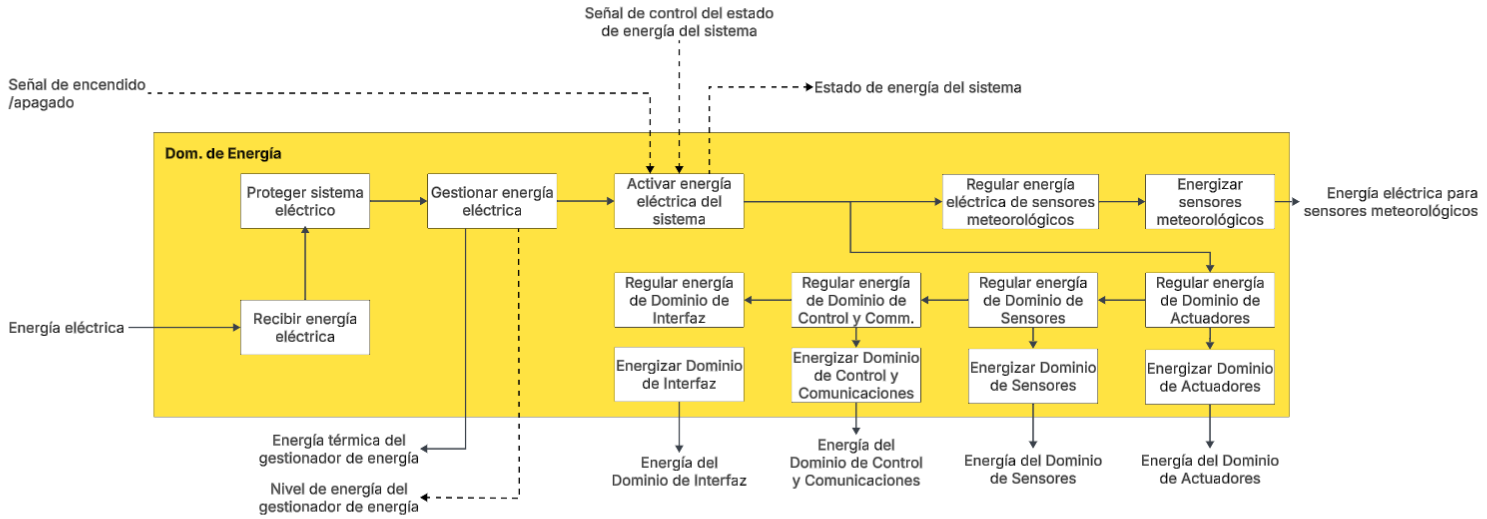
\includegraphics[width=1.2\textwidth]{Imagenes/A3_DominioEnergia.png}
	} \par\medskip
	
	\raggedright
	\footnotesize \textit{Nota.} Elaboración propia.
	\label{fig:Avance3_DomEnergia}
\end{figure}

\subsection{Dominio de Sensores}
El Dominio de Sensores actúa como el sistema de medición y detección del ambiente del robot, encargado de adquirir los estados físicos de los componentes y del entorno inmediato para su posterior procesamiento. Este dominio es alimentado de forma general por el flujo de energía del Dominio de Sensores. Está compuesto de las siguientes funciones:
\begin{enumerate}
	\item \textbf{Sensar temperatura de gestionador de energía:} Capta la energía térmica del gestionador de energía proveniente de dicho módulo y la traduce para emitir los datos brutos de temperatura del gestionador.
	\item \textbf{Sensar nivel de energía:} Lee el nivel de energía del gestionador de energía y lo convierte para entregar los datos brutos del nivel de energía del sistema.
	\item \textbf{Sensar presencia de obstáculo:} Detecta la presencia de obstáculos físicos en la ruta y devuelve la señal de obstáculo encontrado para alertar al control y garantizar su evasión.
	\item \textbf{Sensar velocidad de traslación:} Recibe físicamente la velocidad del mecanismo de traslación y proporciona retroalimentación emitiendo los datos brutos de velocidad.
	\item \textbf{Sensar orientación de plataforma:} Capta el grado de orientación de la plataforma y lo convierte en los datos brutos de orientación de la plataforma para permitir cerrar el lazo de control de la instrumentación.
	\item \textbf{Sensar posición de plataforma:} Recibe la posición de la plataforma física y emite los correspondientes datos brutos de posición de la plataforma.
	\item \textbf{Sensar orientación del sistema:} Capta la orientación del sistema global del vehículo y la transforma para entregar los datos brutos de orientación del sistema para la navegación espacial.
	\item \textbf{Captar señal GPS:} Recibe la señal GPS satelital externa y la devuelve como una señal GPS captada para posibilitar el seguimiento de rutas y geolocalización en el entorno.
\end{enumerate}

\begin{figure}[H]
	\captionsetup{justification=raggedright, singlelinecheck=false, labelsep=none}
	
	\caption[Dominio de sensores de la estructura de funciones.]{} 
	
	\textit{Dominio de sensores de la estructura de funciones.} \par\medskip
	
	\centering
	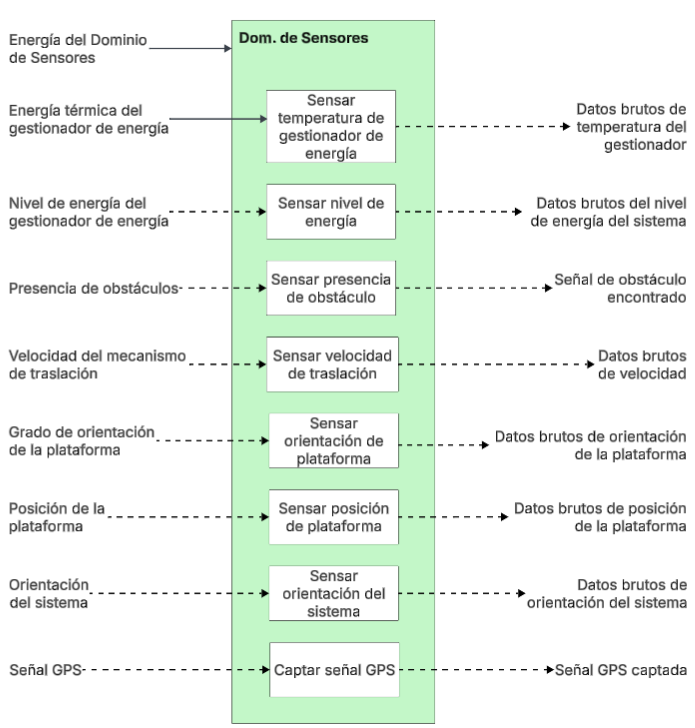
\includegraphics[width=0.8\textwidth]{Imagenes/A3_DominioSensores.png} \par\medskip
	
	\raggedright
	\footnotesize \textit{Nota.} Elaboración propia.
	\label{fig:Avance3_DomSensores}
\end{figure}
\subsection{Dominio de Control}

El Dominio de Control opera como el núcleo lógico y computacional del sistema, encargado de procesar la información recibida, gestionar la seguridad energética, registrar los datos climáticos y comandar tanto la navegación como los actuadores. Todo el subsistema es alimentado por la energía del Dominio de Control y el Dominio de Comunicaciones. Está compuesto de las siguientes funciones:

\begin{enumerate}
	\item \textbf{Procesar datos meteorológicos:} Recibe los datos meteorológicos brutos, enviándolos hacia el exterior como datos meteorológicos procesados y transfiriéndolos simultáneamente al bloque de registro.
	\item \textbf{Registrar datos meteorológicos:} Escribe la información recibida generando el flujo de comunicación con memoria externa de salida para el respaldo físico de los datos.
	\item \textbf{Procesar temperatura de gestionador:} Interpreta los datos brutos de temperatura del gestionador provenientes del módulo de energía.
	\item \textbf{Procesar nivel de energía:} Interpreta los datos brutos del nivel de energía del sistema y emite directamente la información sobre estado de energía hacia el exterior.
	\item \textbf{Procesar estado de energía del sistema:} Recibe y hace converger los flujos lógicos internos de temperatura y nivel de energía procesados para devolver una variable de estado general.
	\item \textbf{Controlar estado de energía del sistema:} Evalúa la variable del bloque anterior para generar la señal de control del estado de energía del sistema, la cual interactúa con el interruptor de encendido.
	\item \textbf{Procesar rutas de inspección:} Extrae la información espacial ingresada desde la comunicación con memoria externa de entrada para generar internamente la información procesada de rutas de inspección.
	\item \textbf{Procesar posición del sistema:} Interpreta los datos de posición del sistema brutos externos para derivar las coordenadas de posición del sistema.
	\item \textbf{Procesar presencia de obstáculo:} Evalúa la señal de obstáculo encontrado proveniente de los sensores, retransmitiéndola de forma directa como salida de alerta y generando internamente la posición de obstáculo.
	\item \textbf{Procesar orientación del sistema:} Recibe e interpreta los datos brutos de orientación del sistema para alimentar los cálculos de navegación espacial.
	\item \textbf{Procesar velocidad de traslación, procesar orientación de la plataforma y procesar posición de la plataforma:} Son tres funciones paralelas que interpretan de forma independiente los datos brutos de velocidad, los datos brutos de orientación de la plataforma y los datos brutos de posición de la plataforma, provenientes de la retroalimentación de los mecanismos físicos.
	\item \textbf{Controlar movimiento de actuador de traslación, orientación de plataforma y posicionamiento de plataforma):} Constituyen las tres etapas finales de salida de este dominio. Integran de forma conjunta las variables de navegación (rutas, coordenadas, orientación del sistema y obstáculos) con sus respectivos lazos de retroalimentación para emitir las señales de control respectivas.
\end{enumerate}

\begin{figure}[H]
	\captionsetup{justification=raggedright, singlelinecheck=false, labelsep=none}
	
	\caption[Dominio de control de la estructura de funciones.]{} 
	
	\textit{Dominio de control de la estructura de funciones.} \par\medskip
	
	\makebox[\textwidth][c]{ 
		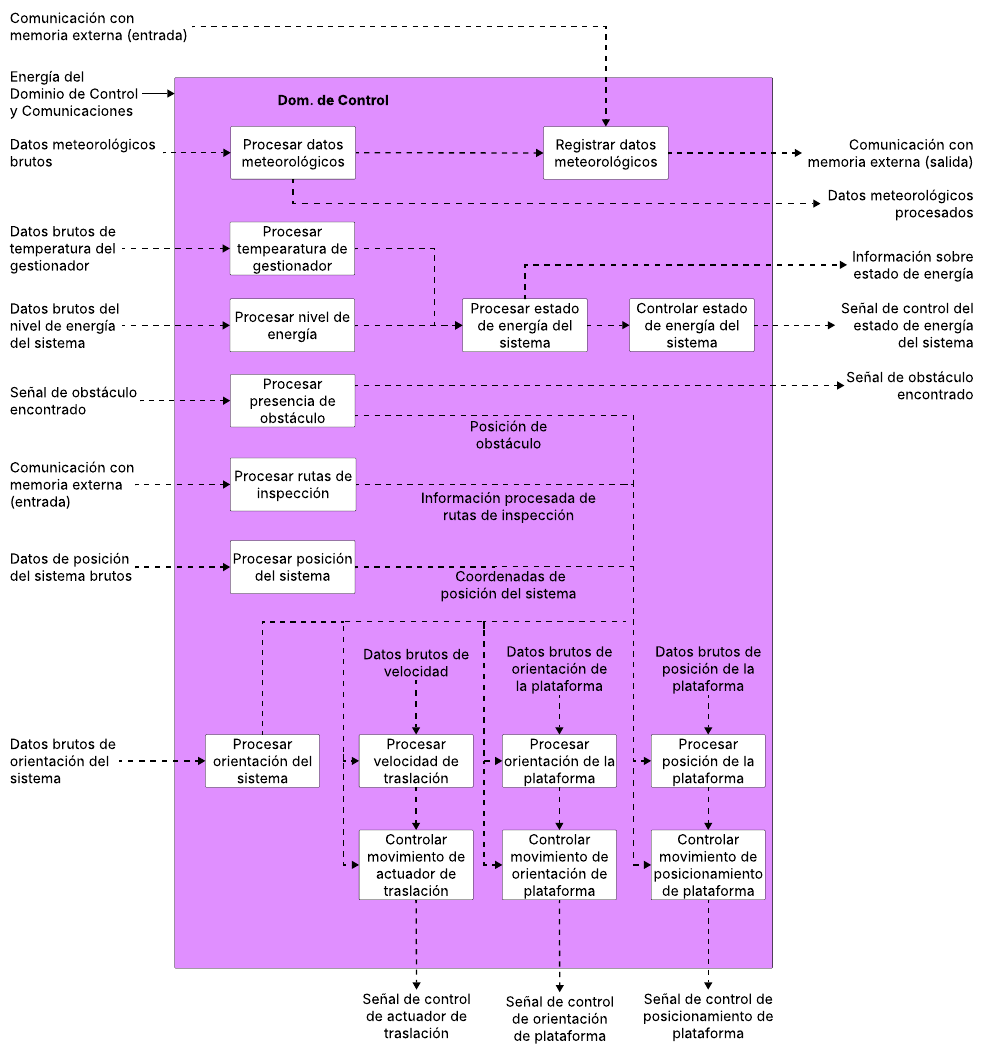
\includegraphics[width=0.9\textwidth]{Imagenes/A3_DominioControl.png}
	} \par\medskip
	
	\raggedright
	\footnotesize \textit{Nota.} Elaboración propia.
	\label{fig:Avance3_DomControl}
\end{figure}

\subsection{Dominio de Comunicación}

El Dominio de Comunicación actúa como el puente de telemetría entre el robot y la red externa del parque fotovoltaico. Para su operatividad, todo este subsistema se encuentra alimentado por el flujo de energía del Dominio de Control y el Dominio de Comunicaciones. El dominio se compone de las siguientes funciones:

\begin{enumerate}
	\item \textbf{Procesar señal GPS recibida:} Capta e interpreta la señal de radiofrecuencia satelital proveniente del entorno para transformarla y entregar los datos de posición del sistema brutos, los cuales son requeridos por la lógica de navegación interna.
	
	\item \textbf{Procesar señal de mando recibida:} Gestiona el enlace interactivo de entrada proveniente de la señal de control de telecomunicación. Principalmente, esta función decodifica la trama de los comandos de telemetría, asegurando una respuesta inmediata del robot frente a instrucciones del usuario.
	
	\item \textbf{Transmitir estado telemétrico:} Emite la señal de estado de transmisión telemétrica hacia el exterior, lo que permite a la estación base monitorear de forma continua la calidad, latencia e integridad del enlace de red con el vehículo.
	
	\item \textbf{Transmitir datos meteorológicos:} Constituye la etapa final del reporte climático y operativo. Esta función recibe los datos meteorológicos procesados desde el dominio de control, y seguidamente codifica y empaqueta la información en un payload para enviarla hacia la estación base en forma de paquetes de datos meteorológicos consolidados.
\end{enumerate}

\begin{figure}[H]
	\captionsetup{justification=raggedright, singlelinecheck=false, labelsep=none}
	
	\caption[Dominio de comunicaciones de la estructura de funciones.]{} 
	
	\textit{Dominio de comunicaciones de la estructura de funciones.} \par\medskip
	
	\makebox[\textwidth][c]{ 
		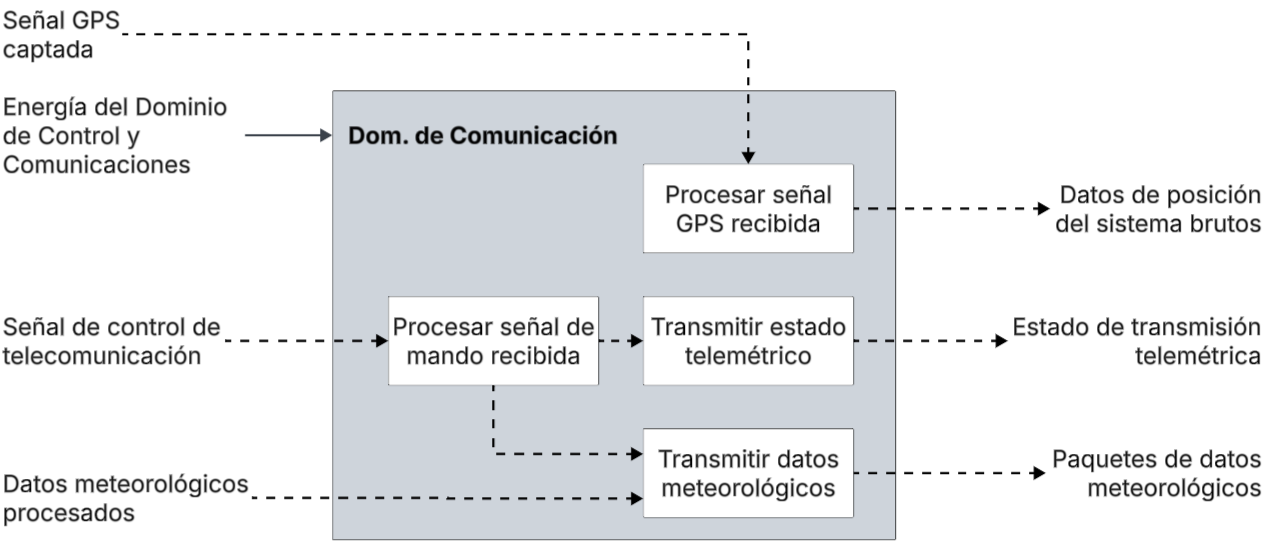
\includegraphics[width=0.8\textwidth]{Imagenes/A3_DominioComunicacion.png}
	} \par\medskip
	
	\raggedright
	\footnotesize \textit{Nota.} Elaboración propia.
	\label{fig:Avance3_DomComunicacion}
\end{figure}

\subsection{Dominio de Interfaz}

El Dominio de Interfaz, mostrado en la \ref{
Avance3_Interfaz} desempeña un rol dual en la arquitectura del robot: por un lado, actúa como el puerto de conexión para la instrumentación climática periférica y, por otro, se encarga de exteriorizar los estados operativos y advertencias críticas hacia el personal en el parque fotovoltaico. Para su funcionamiento general, todos los componentes de este subsistema son alimentados directamente por el flujo de energía del Dominio de Interfaz. El dominio cuenta con los siguientes bloques de función:

\begin{enumerate}
	\item \textbf{Accionar movimiento de traslación:} Recibe la señal de control del actuador de traslación y la transforma en la energía cinética necesaria para ejecutar el desplazamiento principal del robot.
	\item \textbf{Accionar movimiento de orientación de plataforma:} Procesa la señal de control de orientación y genera la energía cinética correspondiente para ajustar este parámetro en la plataforma de medición.
	\item \textbf{Accionar movimiento de posicionamiento de plataforma:} Recibe la señal de control de posicionamiento y la convierte en la energía cinética requerida para el ajuste físico final de la plataforma.
\end{enumerate}

\begin{figure}[H]
	\captionsetup{justification=raggedright, singlelinecheck=false, labelsep=none}
	
	\caption[Dominio de interfaz de la estructura de funciones.]{} 
	
	\textit{Dominio de interfaz de la estructura de funciones.} \par\medskip
	
	\makebox[\textwidth][c]{ 
		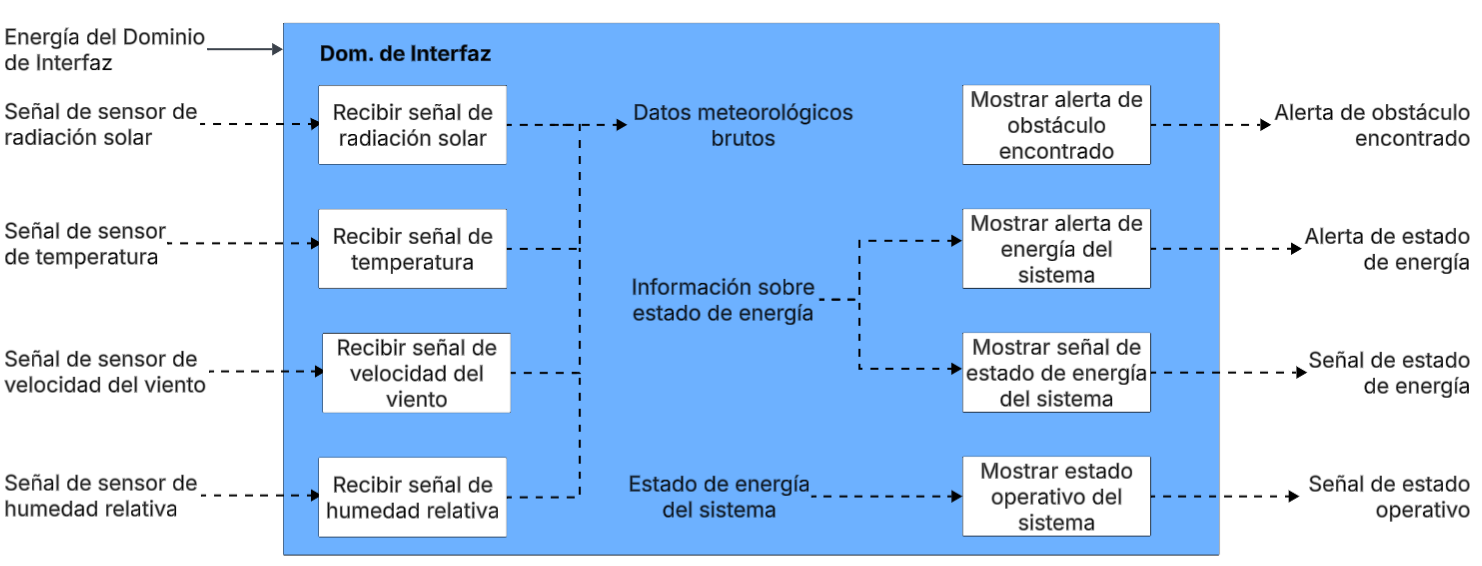
\includegraphics[width=1.0\textwidth]{Imagenes/A3_DominioInterfaz.png}
	} \par\medskip
	
	\raggedright
	\footnotesize \textit{Nota.} Elaboración propia.
	\label{fig:Avance3_DomInterfaz}
\end{figure}

\subsection{Dominio de Actuadores}
El Dominio de Actuadores es el encargado de transformar la energía eléctrica y las instrucciones lógicas en los esfuerzos cinéticos necesarios para la operación física del robot y el ajuste de sus instrumentos. Para su funcionamiento general, todo este subsistema es alimentado por el flujo de energía del Dominio de Actuadores. El dominio se compone de las siguientes funciones:

\begin{enumerate}
	\item \textbf{Accionar movimiento de traslación:} Recibe la señal de control del actuador de traslación y la transforma en la energía cinética necesaria para ejecutar el desplazamiento principal del robot.
	\item \textbf{Accionar movimiento de orientación de plataforma:} Procesa la señal de control de orientación y genera la energía cinética correspondiente para ajustar este parámetro en la plataforma de medición.
	\item \textbf{Accionar movimiento de posicionamiento de plataforma:} Recibe la señal de control de posicionamiento y la convierte en la energía cinética requerida para el ajuste físico final de la plataforma.
\end{enumerate}

\begin{figure}[H]
	\captionsetup{justification=raggedright, singlelinecheck=false, labelsep=none}
	
	\caption[Dominio de actuadores de la estructura de funciones.]{} 
	
	\textit{Dominio de actuadores de la estructura de funciones.} \par\medskip
	
	\centering
	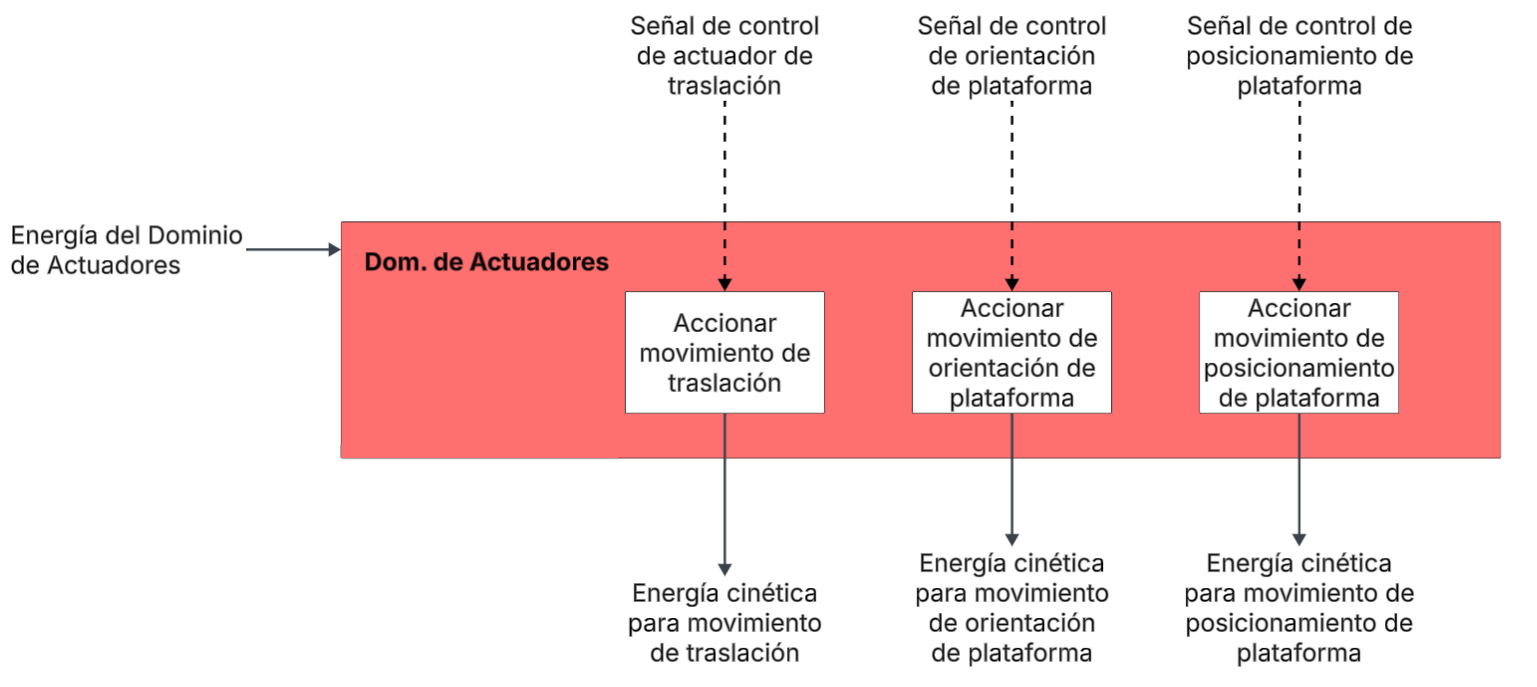
\includegraphics[width=0.99\textwidth]{Imagenes/A3_DominioActuadores.png} \par\medskip
	
	\raggedright
	\footnotesize \textit{Nota.} Elaboración propia.
	\label{fig:Avance3_DomActuadores}
\end{figure}

\subsection{Dominio Mecánico}

El Dominio Mecánico conforma el soporte estructural del vehículo y materializa las interacciones dinámicas y físicas con el entorno del parque solar. Está compuesto de las siguientes funciones:

\begin{enumerate}
	\item \textbf{Soportar plataforma de medición de radiación:} Sostiene la carga física de la instrumentación climática frente a las vibraciones mecánicas del entorno.
	\item \textbf{Proteger componentes internos:} Aísla el equipo para garantizar la integridad de la tecnología frente a factores externos como la suciedad del ambiente.
	\item \textbf{Soportar componentes:} Provee la base física unificada y el soporte estructural estático general para el resto del sistema.
	\item \textbf{Alojar gestionador de energía:} Provee la contención estructural física específica para el gestionador del sistema de energía.
	\item \textbf{Alojar memoria externa:} Actúa como la interfaz material que recibe la memoria externa física. Transmite la comunicación de entrada (rutas de inspección y formatos) al control y recibe la señal de salida para grabar los datos registrados.
	\item \textbf{Generar movimiento de traslación:} Transforma la energía cinética recibida en el desplazamiento general sobre el terreno, retroalimentando al sistema con la velocidad del mecanismo de traslación.
	\item \textbf{Orientar plataforma de medición de radiación:} Utiliza la energía cinética proveniente de los actuadores para ejecutar el cambio de ángulo, entregando como información el grado de orientación de la plataforma.
	\item \textbf{Posicionar plataforma de medición de radiación:} Emplea la energía cinética correspondiente para su ajuste espacial final, suministrando la posición de la plataforma para cerrar los lazos de control y generando las vibraciones emitidas hacia el exterior.
\end{enumerate}
\begin{figure}[H]
	\captionsetup{justification=raggedright, singlelinecheck=false, labelsep=none}
	
	\caption[Dominio mecánico de la estructura de funciones.]{} 
	
	\textit{Dominio mecánico de la estructura de funciones.} \par\medskip
	
	\makebox[\textwidth][c]{ 
		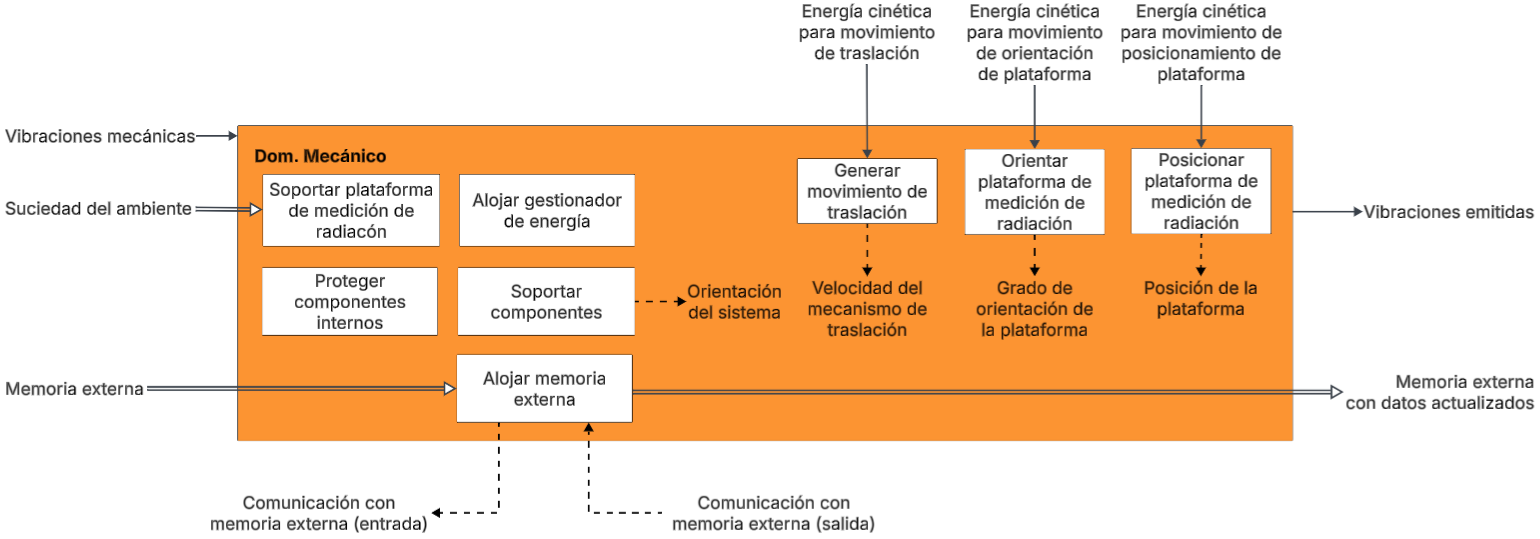
\includegraphics[width=1.25\textwidth]{Imagenes/A3_DominioMecanico.png}
	} \par\medskip
	
	\raggedright
	\footnotesize \textit{Nota.} Elaboración propia.
	\label{fig:Avance3_DomMecanico}
\end{figure}

\section{Matriz Morfológica}

Una vez completada la abstracción del sistema en la Estructura de Funciones, se procede con la búsqueda sistemática de principios de solución clasificados en la Matriz Morfológica, que permite desglosar las funciones elementales y proponer para cada una de distintos portadores de función o alternativas tecnológicas. El objetivo de esta sección es establecer un abanico amplio de principios físicos, mecánicos, electrónicos y de software que sean capaces de resolver las tareas del robot, para posteriormente combinarlos y generar los conceptos de solución integrales.
% --- Dominio de Energía ---
\begin{center}
	\footnotesize
	\begin{xltabular}{\textwidth}{|p{3.5cm}|>{\centering\arraybackslash}X|>{\centering\arraybackslash}X|>{\centering\arraybackslash}X|}
		\caption{Matriz Morfológica del Dominio de Energía.}
		\label{tab:matriz_energia} \\
		\hline
		\rowcolor[HTML]{D9E1F2} 
		\textbf{Función Parcial} & \textbf{Solución 1} & \textbf{Solución 2} & \textbf{Solución 3} \\ \hline
		\endfirsthead
		
		\multicolumn{4}{c}%
		{{\bfseries \tablename\ \thetable{} -- Continuación de la página anterior}} \\
		\hline
		\rowcolor[HTML]{D9E1F2} 
		\textbf{Función Parcial} & \textbf{Solución 1} & \textbf{Solución 2} & \textbf{Solución 3} \\ \hline
		\endhead
		
		\hline
		\endfoot
		
		\hline
		\endlastfoot
		
		\textbf{1. Recibir energía eléctrica} & 
		Conector Plug Jack DC \par\smallskip 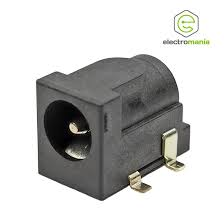
\includegraphics[width=0.7\linewidth]{ImagenesMatriz/ConectorPlugJackDC.jpg} & 
		Conector de alta corriente XT60 \par\smallskip 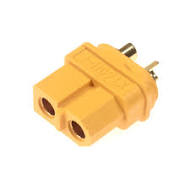
\includegraphics[width=0.7\linewidth]{ImagenesMatriz/ConectorAltaCorriente.jpg} & 
		Contactos magnéticos \par\smallskip 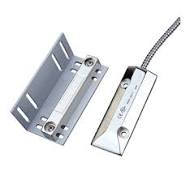
\includegraphics[width=0.7\linewidth]{ImagenesMatriz/ConectorContactoMagnetico.jpg} \\ \hline
		
		\textbf{2. Proteger sistema eléctrico} & 
		Fusible cerámico de cartucho \par\smallskip 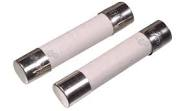
\includegraphics[width=0.7\linewidth]{ImagenesMatriz/FusibleCeramico.jpg} & 
		Fusible electrónico eFuse \par\smallskip 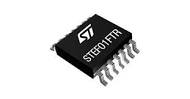
\includegraphics[width=0.9\linewidth]{ImagenesMatriz/eFuse.jpg} & 
		Disyuntor termomagnético \par\smallskip 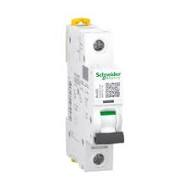
\includegraphics[width=0.7\linewidth]{ImagenesMatriz/DisyuntorTermomagnetico.jpg} \\ \hline
		
		\textbf{3. Gestionar energía eléctrica} & 
		Batería NiMH + Battery Management System \par\smallskip 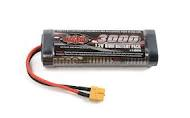
\includegraphics[width=0.7\linewidth]{ImagenesMatriz/NiMh.jpg} & 
		Batería LiIon + Battery Management System \par\smallskip 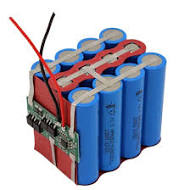
\includegraphics[width=0.7\linewidth]{ImagenesMatriz/LiIon.jpg} & 
		Batería LiPO + Battery Management System \par\smallskip 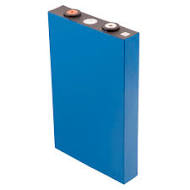
\includegraphics[width=0.7\linewidth]{ImagenesMatriz/LiPo.jpg} \\ \hline
		
		\textbf{4. Activar energía eléctrica} & 
		Seccionador rotativo manual \par\smallskip 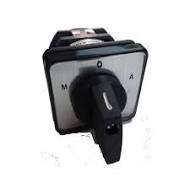
\includegraphics[width=0.7\linewidth]{ImagenesMatriz/Rotativo.jpg} & 
		Relé de estado sólido \par\smallskip 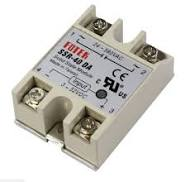
\includegraphics[width=0.7\linewidth]{ImagenesMatriz/ReleEstadoSolido.jpg} & 
		Contactor mecánico \par\smallskip 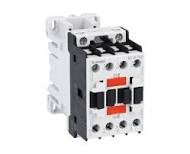
\includegraphics[width=0.7\linewidth]{ImagenesMatriz/Contactor.jpg} \\ \hline
		
		\textbf{5. Regular energía de Interfaz} \vspace{0.2cm} & 
		\multirow{3}{=}{\centering Regulador de bomba de carga fija\par\vspace{0.2cm} 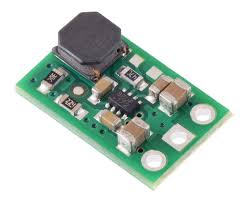
\includegraphics[width=0.65\linewidth]{ImagenesMatriz/PumpChargeRegulador.jpg}} & 
		\multirow{3}{=}{\centering Regulador lineal LDO \par\vspace{0.2cm} 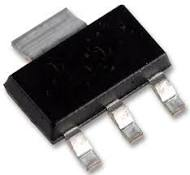
\includegraphics[width=0.65\linewidth]{ImagenesMatriz/ReguladorLDO.jpg}} & 
		\multirow{3}{=}{\centering Regulador Shunt \par\vspace{0.2cm} 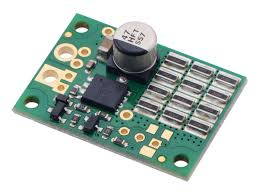
\includegraphics[width=0.65\linewidth]{ImagenesMatriz/ShuntRegulator.jpg}} \\ \cline{1-1}
		
		\textbf{6. Regular energía de Control/Comunicación} \vspace{0.2cm} & & & \\ \cline{1-1}
		
		\textbf{7. Regular energía de Sensores} \vspace{0.6cm} & & & \\ \hline
		%
		\textbf{8. Regular energía de Actuadores} & 
		Convertidor Buck DC-DC \par\smallskip 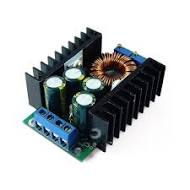
\includegraphics[width=0.7\linewidth]{ImagenesMatriz/ConvertidorBuck.jpg} & 
		Regulador de bomba de carga \par\smallskip 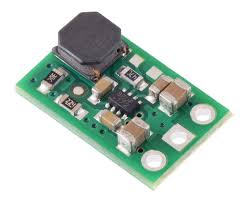
\includegraphics[width=0.7\linewidth]{ImagenesMatriz/PumpChargeRegulador.jpg} & 
		Regulador lineal LDO \par\smallskip 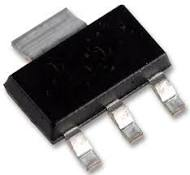
\includegraphics[width=0.7\linewidth]{ImagenesMatriz/ReguladorLDO.jpg} \\ \hline
		%
		\pagebreak
		
		% --- INICIO BLOQUE 5-8 ---
		\textbf{9. Energizar Interfaz} \vspace{0.6cm} & 
		\multirow{3}{=}{\centering Cable trenzado estándar \par\vspace{0.2cm} 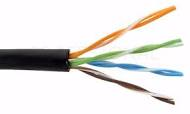
\includegraphics[width=0.65\linewidth]{ImagenesMatriz/CableTrenzado.jpg}} & 
		\multirow{3}{=}{\centering Conectores circular roscado \par\vspace{0.2cm} 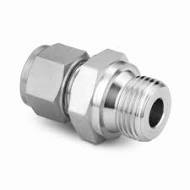
\includegraphics[width=0.65\linewidth]{ImagenesMatriz/ConectorRoscado.jpg}} & 
		\multirow{3}{=}{\centering Barras colectoras Busbars \par\vspace{0.2cm} 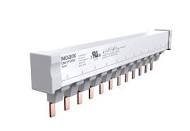
\includegraphics[width=0.65\linewidth]{ImagenesMatriz/Busbar.jpg}} \\ \cline{1-1}
		
		\textbf{10. Energizar Control/Comm.} \vspace{0.6cm} & & & \\ \cline{1-1}
		
		\textbf{11. Energizar Sensores} \vspace{0.6cm} & & & \\ \hline
		% --- FIN BLOQUE 9-11 ---
		
		\textbf{12. Energizar Actuadores} & 
		Cable de Baja Tensión \par\smallskip 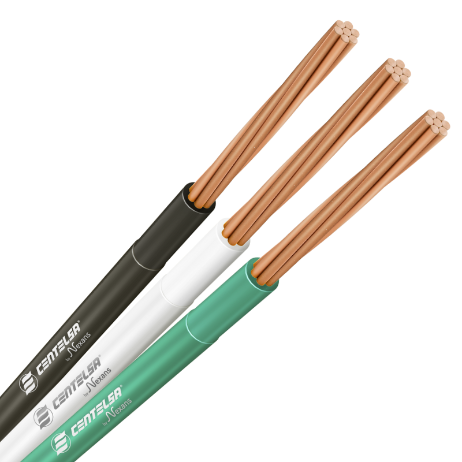
\includegraphics[width=0.7\linewidth]{ImagenesMatriz/CableBajaTension.png} & 
		Conector Circular Roscado \par\smallskip 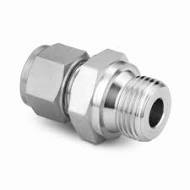
\includegraphics[width=0.7\linewidth]{ImagenesMatriz/ConectorRoscado.jpg} & 
		Barras colectoras Busbars \par\smallskip 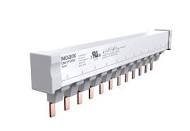
\includegraphics[width=0.7\linewidth]{ImagenesMatriz/Busbar.jpg} \\ \hline
		%%
		\textbf{13. Regular energía eléctrica de sensores meteorológicos} & 
		Regulador de bomba de carga \par\smallskip 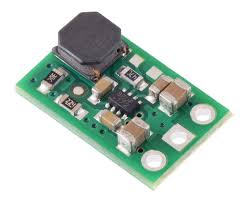
\includegraphics[width=0.7\linewidth]{ImagenesMatriz/PumpChargeRegulador.jpg} & 
		Regulador lineal LDO \par\smallskip 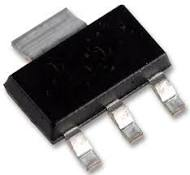
\includegraphics[width=0.7\linewidth]{ImagenesMatriz/ReguladorLDO.jpg} & 
		Regulador Shunt \par\smallskip 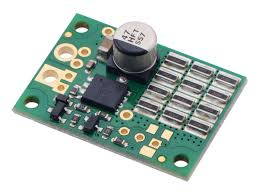
\includegraphics[width=0.7\linewidth]{ImagenesMatriz/ShuntRegulator.jpg} \\ \hline
		%%
		\textbf{14. Energizar  sensores meteorológicos} & 
		Cable trenzado estándar \par\smallskip 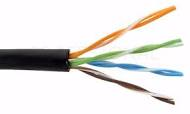
\includegraphics[width=0.7\linewidth]{ImagenesMatriz/CableTrenzado.jpg} & 
		Conector circular roscado \par\smallskip 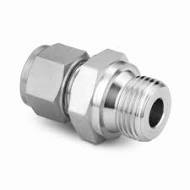
\includegraphics[width=0.7\linewidth]{ImagenesMatriz/ConectorRoscado.jpg} & 
		Barras colectoras Busbars \par\smallskip 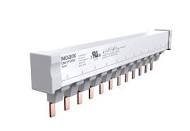
\includegraphics[width=0.7\linewidth]{ImagenesMatriz/Busbar.jpg} \\ \hline
		
	\end{xltabular}
\end{center}

\begin{itemize}
	\item \textbf{Recibir energía eléctrica:} para esta función se evaluó el conector Plug Jack DC, que permite una conexión lineal simple para corrientes medias; el conector de alta corriente XT60, el cual asegura una conexión física firme capaz de soportar las altas corrientes requeridas para la carga de baterías; y los contactos magnéticos, que facilitan un acople automático con la estación de carga sin requerir movimientos de gran exactitud por parte del vehículo.
	
	\item \textbf{Proteger sistema eléctrico:} se analizó el fusible electrónico eFuse por su corte rápido y posibilidad de restablecimiento automático, ideal para sistemas autónomos; el disyuntor termomagnético, que ofrece una protección robusta ante cortocircuitos pero exige rearme manual; y el fusible cerámico de cartucho, una opción de bajo costo y alta capacidad de ruptura que requiere reemplazo físico tras activarse.
	
	\item \textbf{Gestionar energía eléctrica:} las opciones contemplan la batería LiPO con Battery Management System (BMS), destacada por sus altas tasas de descarga y bajo peso; la batería LiIon con BMS, que proporciona una alta densidad energética y larga vida útil para asegurar la autonomía de operación del robot; y la batería NiMH con BMS, una alternativa estable frente a riesgos térmicos pero con la desventaja de tener un mayor peso y menor densidad de energía.
	
	\item \textbf{Activar energía eléctrica:} se consideró el relé de estado sólido, que permite la conmutación mediante señales de control sin partes móviles; el contactor mecánico, útil para manejar los picos de corriente durante el arranque de los motores; y el seccionador rotativo manual, que actúa como un elemento de corte físico directo para asegurar la desconexión total.
	
	\item \textbf{Regular energía Interfaz, Regular energía Control/Comm, Regular energía Sensores y Regular energía eléctrica de sensores meteorológicos:} se evaluó el regulador Shunt, de diseño simple pero térmicamente ineficiente al disipar el exceso de energía como calor; el regulador lineal LDO, que ofrece un voltaje de salida estable y con bajo ruido eléctrico, indispensable para los microcontroladores y la instrumentación; y el regulador de bomba de carga, útil para elevar o reducir voltajes en espacios reducidos pero limitado a bajas corrientes.
	
	\item \textbf{Regular energía de Actuadores:} para esta etapa de regulación de potencia se analizó el regulador lineal LDO, que entrega un voltaje limpio pero genera demasiada pérdida térmica frente a la demanda de los motores; el regulador de bomba de carga, de circuito compacto pero con capacidad de corriente insuficiente; y el convertidor Buck DC-DC, que posee una alta eficiencia de conversión energética para soportar el consumo dinámico de los mecanismos mecánicos.
	
	\item \textbf{Energizar Interfaz, Energizar Control/Comm., Energizar Sensores y Energizar sensores meteorológicos:} se propusieron las barras colectoras para facilitar una distribución rígida de alimentación entre componentes fijos; el cable trenzado estándar, que aporta flexibilidad para el ruteo interno en la caja de control; y la combinación de conectores circulares roscados con barras colectoras, que garantiza una conexión firme y resistente a las desconexiones causadas por las vibraciones del terreno.
	
	\item \textbf{Energizar Actuadores (Distribución):} se consideraron los contactos magnéticos, de acople rápido pero vulnerables a perder continuidad por los impactos del movimiento; el cable trenzado estándar, que proporciona la tolerancia mecánica necesaria para llevar la energía hasta los ejes móviles de los actuadores; y las barras colectoras Busbars, que soportan altas corrientes de manera eficiente y robusta.
\end{itemize}


\subsection{Dominio de Sensores}


\begin{center}
	\footnotesize
	\begin{xltabular}{\textwidth}{|p{3.5cm}|>{\centering\arraybackslash}X|>{\centering\arraybackslash}X|>{\centering\arraybackslash}X|}
		\caption{Matriz Morfológica del Dominio de Sensores.}
		\label{tab:matriz_sensores} \\
		\hline
		\rowcolor[HTML]{D9E1F2} 
		\textbf{Función Parcial} & \textbf{Solución 1} & \textbf{Solución 2} & \textbf{Solución 3} \\ \hline
		\endfirsthead
		
		\multicolumn{4}{c}%
		{{\bfseries \tablename\ \thetable{} -- Continuación de la página anterior}} \\
		\hline
		\rowcolor[HTML]{D9E1F2} 
		\textbf{Función Parcial} & \textbf{Solución 1} & \textbf{Solución 2} & \textbf{Solución 3} \\ \hline
		\endhead
		
		\hline
		\endfoot
		
		\hline
		\endlastfoot
		
		\textbf{1. Sensar temperatura del gestionador} & 
		Termistor NTC \par\smallskip 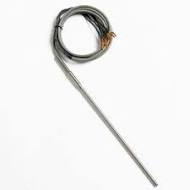
\includegraphics[width=0.7\linewidth]{ImagenesMatriz/TermistorNTC.jpg} & 
		Termopar tipo K \par\smallskip 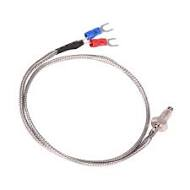
\includegraphics[width=0.7\linewidth]{ImagenesMatriz/Termopar.jpg} & 
		Sensor RTD PT100 \par\smallskip 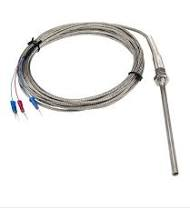
\includegraphics[width=0.7\linewidth]{ImagenesMatriz/SensorRTD.jpg} \\ \hline
		
		\textbf{2. Sensar nivel de energía del gestionador} & 
		Detector de umbral de voltaje \par\smallskip 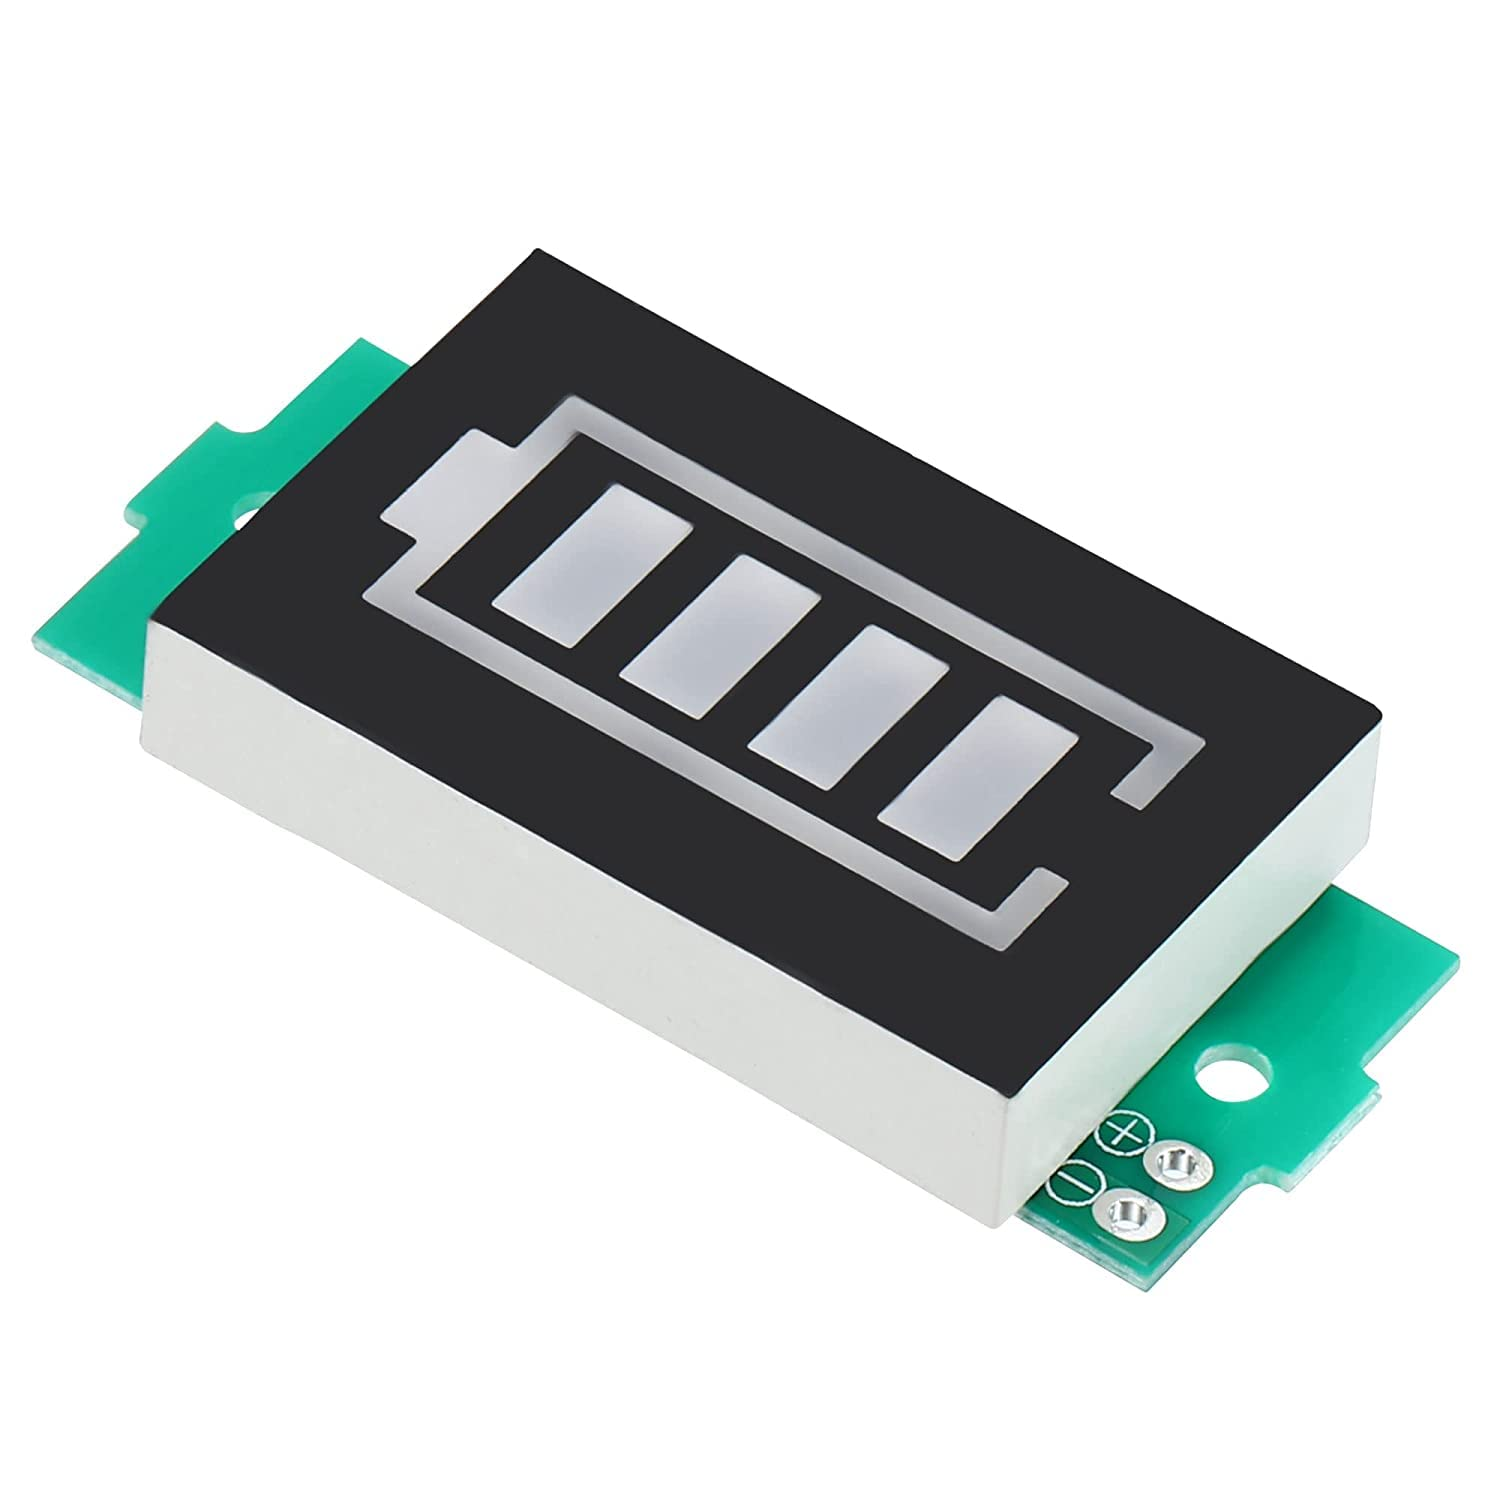
\includegraphics[width=0.7\linewidth]{ImagenesMatriz/SensorNivelVoltaje.jpg}& 
		Sensor contador de Culombios \par\smallskip 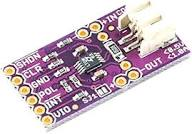
\includegraphics[width=0.7\linewidth]{ImagenesMatriz/SensorNivelCoulomb.jpg} & 
		Sensor de impedancia interna \par\smallskip 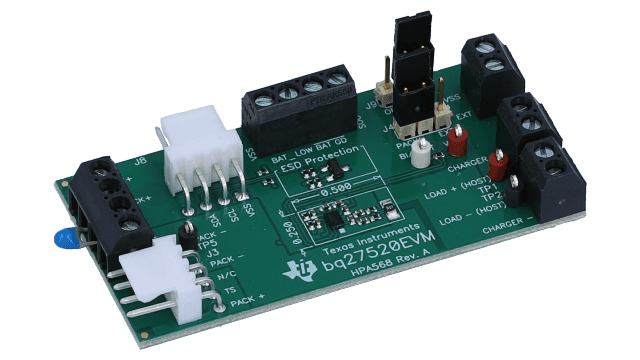
\includegraphics[width=0.9\linewidth]{ImagenesMatriz/SensorNivelImpedencia.png} \\ \hline
		
		\textbf{3. Sensar presencia de obstáculo} & 
		Sensor 3D de tiempo de vuelo \par\smallskip 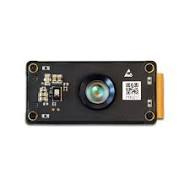
\includegraphics[width=0.7\linewidth]{ImagenesMatriz/SensorToF.jpg}& 
		Módulo CMOS \par\smallskip 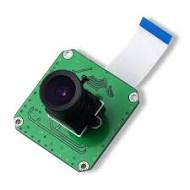
\includegraphics[width=0.7\linewidth]{ImagenesMatriz/CMOSModule.jpg} & 
		Sensor LiDAR 3D \par\smallskip 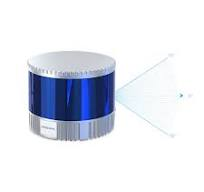
\includegraphics[width=0.9\linewidth]{ImagenesMatriz/LIDAR3D.jpg} \\ \hline
		
		\textbf{4. Sensar velocidad de traslación} & 
		Encoder rotativo incremental\par\smallskip 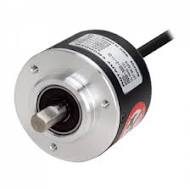
\includegraphics[width=0.7\linewidth]{ImagenesMatriz/EncoderRotativoIncremental.jpg} & 
		Unidad IMU de 9 ejes \par\smallskip 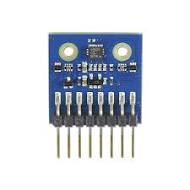
\includegraphics[width=0.7\linewidth]{ImagenesMatriz/IMU9Ejes.jpg} & 
		Radar de onda continua \par\smallskip 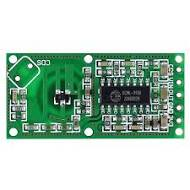
\includegraphics[width=0.7\linewidth]{ImagenesMatriz/RadarOndaContinua.jpg} \\ \hline
		
		\textbf{5. Sensar orientación plataforma} & 
		Sensor de distancia por tiempo de vuelo \par\smallskip 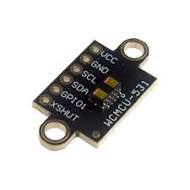
\includegraphics[width=0.7\linewidth]{ImagenesMatriz/SensorDistanciaToF.jpg} & 
		Unidad IMU de 9 ejes \par\smallskip 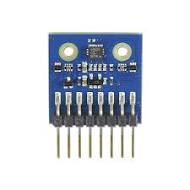
\includegraphics[width=0.7\linewidth]{ImagenesMatriz/IMU9Ejes.jpg} & 
		Encoder rotativo absoluto \par\smallskip 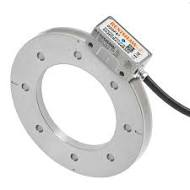
\includegraphics[width=0.7\linewidth]{ImagenesMatriz/EncoderRotativoAbsoluto.jpg} \\ \hline
		
		\textbf{6. Sensar posición de plataforma} & 
		Sensor de fin de carrera \par\smallskip 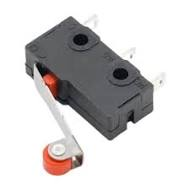
\includegraphics[width=0.7\linewidth]{ImagenesMatriz/FinDeCarrera.jpg} & 
		Potenciómetro lineal \par\bigskip 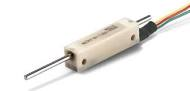
\includegraphics[width=0.7\linewidth]{ImagenesMatriz/PotenciometroLineal.jpg}& 
		Sensor de ultrasonido \par\smallskip 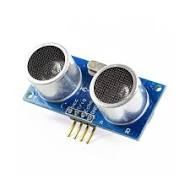
\includegraphics[width=0.7\linewidth]{ImagenesMatriz/SensorUltrasonido.jpg} \\ \hline
		
		\textbf{7. Captar señal GPS} & 
		Antena de circuito flexible \par\smallskip 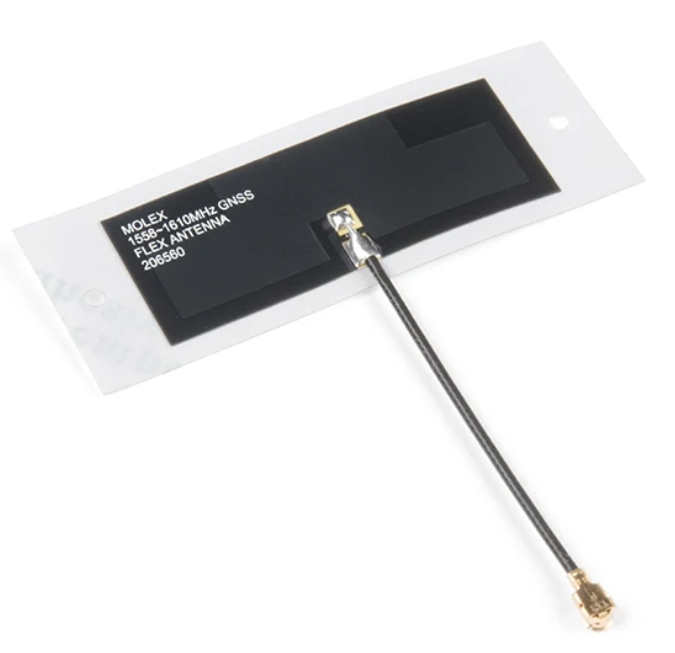
\includegraphics[width=0.7\linewidth]{ImagenesMatriz/AntenaFlexible.png} & 
		Antena de parche cerámico \par\smallskip 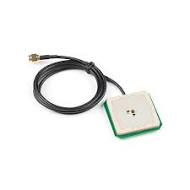
\includegraphics[width=0.7\linewidth]{ImagenesMatriz/AntenaGNSS.jpg} & 
		Antena GPS RTK \par\smallskip 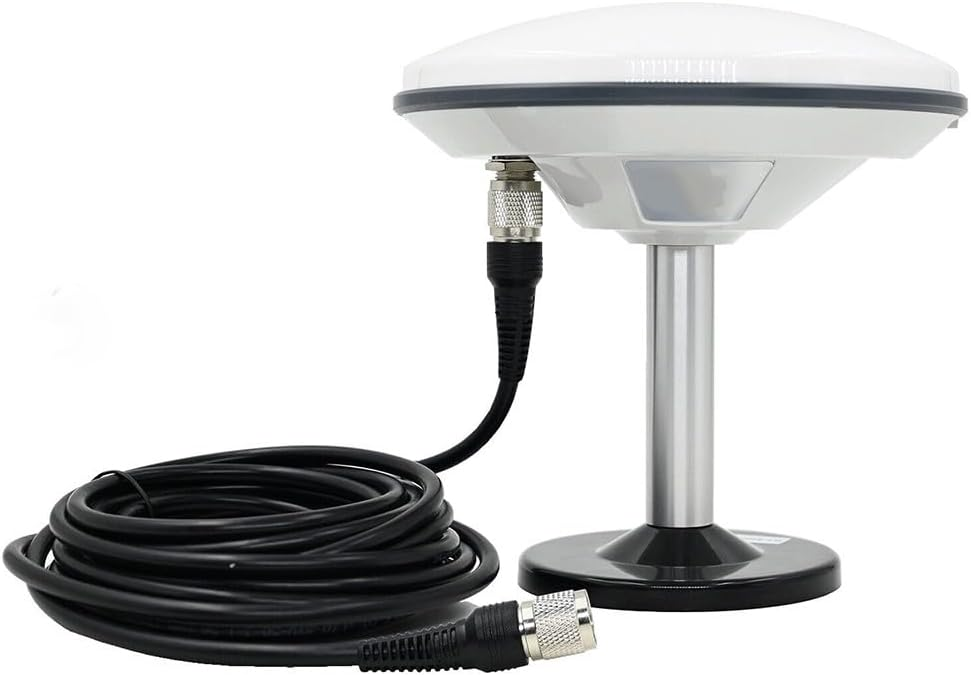
\includegraphics[width=0.7\linewidth]{ImagenesMatriz/AntenaGPSRTK.jpg} \\ \hline
		
		\textbf{8. Sensar orientación del sistema} & 
		\par\smallskip Unidad IMU de 9 ejes 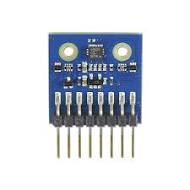
\includegraphics[width=0.7\linewidth]{ImagenesMatriz/IMU9Ejes.jpg} & 
		\par\smallskip Unidad IMU de 9 ejes  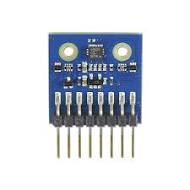
\includegraphics[width=0.7\linewidth]{ImagenesMatriz/IMU9Ejes.jpg} & 
		Matriz de sensores de distancia por tiempo de vuelo \par\smallskip 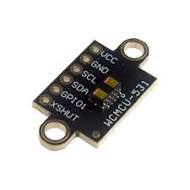
\includegraphics[width=0.7\linewidth]{ImagenesMatriz/SensorDistanciaToF.jpg} \\ \hline
		
	\end{xltabular}
\end{center}


\begin{itemize}
	\item \textbf{Sensar temperatura del gestionador:} Se evaluó el termistor NTC; el sensor RTD PT100, justificado por la necesidad de medir con precisión frente al efecto de isla de calor fotovoltaica (PVHI) y las variaciones térmicas extremas documentadas en la caracterización de microclimas \citep{Armstrong2026, Garcia2014}; y el termopar tipo K, de alta robustez mecánica.
	
	\item \textbf{Sensar nivel de energía del gestionador:} Se consideró el detector de umbral de voltaje, el cual generaría lecturas erróneas debido a las severas caídas de tensión que sufren las baterías al superar pendientes del 28\,\% \citep{GarciaSalinas2025}; el sensor de impedancia; y el contador de Culombios, principio tecnológico clave integrado en los avanzados Sistemas de Gestión de Baterías (BMS) de las estaciones meteorológicas \textit{IoT} evaluadas en el estado del arte para operar en terrenos remotos \citep{SK302020A3}.
	
	\item \textbf{Sensar presencia de obstáculo:} Se consideró el módulo \textit{CMOS}, útil para la generación de mapas espaciales \citep{CN119665962A} pero vulnerable al deslumbramiento por el albedo de los paneles; el sensor \textit{ToF} 3D; y el sensor \textit{LiDAR} 3D, tecnología indispensable extraída de los vehículos terrestres de inspección en desiertos (UGV), ya que es el único principio capaz de evadir zanjas erosivas y relieve complejo que la visión artificial simple no detecta \citep{CN221163061U, Figgis2025}.
	
	\item \textbf{Sensar velocidad de traslación:} Se analizó el \textit{encoder} rotativo incremental, el cual presentará errores críticos de odometría debido al deslizamiento de las orugas en terrenos irregulares, una limitación comprobada en los actuales vehículos de inspección solar \citep{Figgis2025}; el radar de onda continua; y la unidad \textit{IMU} de 9 ejes, requerida para la estimación inercial sin contacto con el suelo.
	
	\item \textbf{Sensar orientación (Plataforma y Sistema):} Se evaluaron el \textit{encoder} rotativo absoluto y el sensor \textit{ToF}; así como la unidad \textit{IMU} de 9 ejes. Este último es el principio técnico fundamental utilizado por las estaciones meteorológicas fotovoltaicas móviles para proveer el vector de gravedad absoluto, activar los mecanismos de nivelación \citep{CN216956405U} y asegurar la horizontalidad de la instrumentación exigida por la norma \citep{IEC61724-1_2021}.
	
	\item \textbf{Sensar posición de plataforma:} Se propuso el potenciómetro lineal; el sensor de ultrasonido, cuyo principio acústico resulta ineficiente al ser desviado por las cargas de viento extremo y las turbulencias aerodinámicas documentadas en las laderas de los parques solares \citep{Xu2024}; y el sensor de fin de carrera, seleccionado por su fiabilidad física a la intemperie.
	
	\item \textbf{Captar señal GPS:} Se evaluó la antena de parche cerámico, propensa a perder satélites al inclinarse en el relieve; la antena de circuito flexible; y la antena \textit{GPS RTK} (Real-Time Kinematic), a menudo combinada con telemetría en vehículos de inspección \citep{CN116405876A}. Su inclusión se justifica al ser la única tecnología capaz de garantizar la exactitud centimétrica indispensable para la georreferenciación de los microclimas y la corrección de ruta en la montaña \citep{Armstrong2026, Figgis2025}.
\end{itemize}


\begin{itemize}
	\item \textbf{Sensar temperatura del gestionador:} para esta función se evaluó el termistor NTC, con un bajo costo y una excelente sensibilidad para los rangos de temperatura de operación esperados en las baterías; el sensor RTD PT100, el cual brinda una alta precisión y estabilidad térmica a cambio de un mayor costo y un circuito de acondicionamiento más complejo; y el termopar tipo K, que es muy robusto y soporta rangos térmicos extremos, aunque puede presentar menor exactitud a temperatura ambiente.
	
	\item \textbf{Sensar nivel de energía del gestionador:} se consideró el sensor contador de Culombios, que permite una medición exacta del estado de carga al integrar la corriente en el tiempo; el detector de umbral de voltaje, una opción simple y económica pero cuya limitación generará lecturas falsas por las caídas de tensión al demandar alta corriente para escalar pendientes de hasta el 28\,\% \citep{GarciaSalinas2025};; y el sensor de impedancia interna, el cual es ideal para evaluar la salud y degradación de la celda a largo plazo, pero resulta complejo de implementar para mediciones continuas en operación.
	
	\item \textbf{Sensar presencia de obstáculo:} las alternativas contemplan el sensor LiDAR 3D, que otorga alta precisión y un amplio rango para el mapeo espacial, pero exige un alto costo y capacidad de procesamiento; el módulo CMOS, muy útil para la clasificación visual de los obstáculos mediante algoritmos, aunque susceptible a los deslumbramientos y reflejos propios de los paneles solares; y el sensor 3D de tiempo de vuelo, que ofrece una buena percepción de profundidad a distancias cortas y medias con una menor carga computacional.
	
	\item \textbf{Sensar velocidad de traslación:} para la retroalimentación del movimiento se analizó el encoder rotativo incremental, que proporciona una medición mecánica directa, aunque sus lecturas pueden falsearse si las ruedas deslizan; la unidad IMU de 9 ejes, que estima la velocidad sin depender de la tracción mecánica pero sufre requiere calibración y reajuste de mantenimiento; y el radar de onda continua, el cual mide la velocidad real respecto al suelo mediante el efecto Doppler, siendo totalmente inmune al deslizamiento y al polvo, aunque más costoso.
	
	\item \textbf{Sensar orientación plataforma y Sensar orientación del sistema:} se evaluó el encoder rotativo absoluto, que brinda una alta precisión para medir los ángulos articulares y retiene su posición incluso ante cortes de energía; la unidad IMU de 9 ejes, que permite obtener la orientación espacial general sin necesidad de acoples mecánicos físicos, aunque es susceptible a vibraciones e interferencias magnéticas; y el sensor de distancia por tiempo de vuelo (ToF), capaz de inferir la inclinación midiendo distancias sin contacto, pero con menor exactitud para un control rotacional estricto.
	
	\item \textbf{Sensar posición de plataforma:} se consideró el sensor de ultrasonido, una alternativa económica de medición de distancia sin contacto que, sin embargo, puede verse afectada por las corrientes de viento; el sensor de fin de carrera, que ofrece una detección de topes físicos muy robusta y simple, pero está restringida a estados discretos sin brindar una lectura continua; y el potenciómetro lineal, que entrega una retroalimentación analógica continua de la posición física, aunque sus partes móviles son vulnerables al desgaste por la suciedad del entorno.
	
	\item \textbf{Captar señal GPS:} las opciones para la recepción satelital incluyen la antena de parche cerámico, que es compacta, económica y estandarizada, pero exige una orientación estrictamente cenital y un buen plano de tierra; la antena \textit{GPS RTK} (Real-Time Kinematic), a menudo combinada con telemetría en vehículos de inspección \citep{CN116405876A}, que garantiza una exactitud indispensable para el mapeo de posición del robot en topografías complejas ; y la antena de circuito flexible, que se adapta fácilmente a la geometría interna del vehículo, pero sacrifica ganancia y eficiencia general de recepción.
	
\end{itemize}
\pagebreak
\subsection{Dominio de Control}

% --- Tabla de Control (Hardware) ---
\begin{center}
	\footnotesize
	\begin{xltabular}{\textwidth}{|p{3.5cm}|>{\centering\arraybackslash}X|>{\centering\arraybackslash}X|>{\centering\arraybackslash}X|}
		\caption{Matriz Morfológica del Dominio de Control (Hardware).}
		\label{tab:matriz_control_hw} \\
		\hline
		\rowcolor[HTML]{D9E1F2} 
		\textbf{Función Parcial} & \textbf{Solución 1} & \textbf{Solución 2} & \textbf{Solución 3} \\ \hline
		\endfirsthead
		\multicolumn{4}{c}%
		{{\bfseries \tablename\ \thetable{} -- Continuación de la página anterior}} \\
		\hline
		\rowcolor[HTML]{D9E1F2} 
		\textbf{Función Parcial} & \textbf{Solución 1} & \textbf{Solución 2} & \textbf{Solución 3} \\ \hline
		\endhead
		\hline
		\endfoot
		\hline
		\endlastfoot
		% --- INICIO BLOQUE MASIVO DE 10 FILAS ---
		\textbf{1. Procesar datos meteorológicos} & 
		\multirow{13}{=}{\centering Microcontrolador \par\vspace{0.2cm} 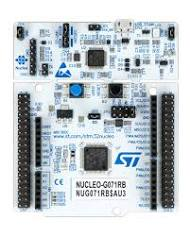
\includegraphics[width=\linewidth]{ImagenesMatriz/Microcontrolador.jpg}} & 
		\multirow{13}{=}{\centering Placa SBC \par\vspace{0.2cm} 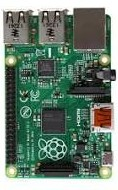
\includegraphics[width=0.7\linewidth]{ImagenesMatriz/SBC.jpg}} & 
		\multirow{13}{=}{\centering PLC \par\vspace{0.2cm} 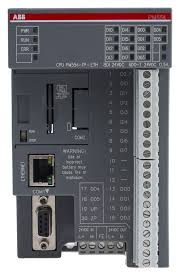
\includegraphics[width=0.7\linewidth]{ImagenesMatriz/PLC.jpg}} \\ \cline{1-1}
		\textbf{2. Procesar temperatura del gestionador} & & & \\ \cline{1-1}
		\textbf{3. Procesar nivel energía del gestionador} & & & \\ \cline{1-1}
		\textbf{4. Procesar estado energía del gestionador} & & & \\ \cline{1-1}
		\textbf{5. Procesar velocidad de traslación} & & & \\ \cline{1-1}
		\textbf{6. Procesar orientación de plataforma} & & & \\ \cline{1-1}
		\textbf{7. Procesar posición de plataforma} & & & \\ \cline{1-1}
		\textbf{8. Controlar estado energía del gestionador} & & & \\ \cline{1-1}
		\textbf{9. Controlar movimiento de traslación} & & & \\ \cline{1-1}
		\textbf{10. Controlar movimiento de orientación de plataforma} & & & \\ \cline{1-1}
		\textbf{11. Controlar posicionamiento de plataforma} & & & \\ \cline{1-1}
		\textbf{12. Controlar posicionamiento de plataforma} & & & \\ \cline{1-1} 
		\textbf{13. Procesar dirección de traslación} & & & \\ \hline
		% --- FILAS INDIVIDUALES ---
		\textbf{14. Procesar señal de obstáculo} & 
		Microcontrolador \par\smallskip 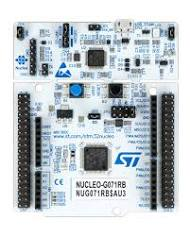
\includegraphics[width=0.7\linewidth]{ImagenesMatriz/Microcontrolador.jpg} & 
		Placa SBC \par\smallskip 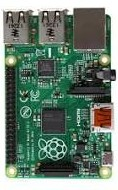
\includegraphics[width=0.7\linewidth]{ImagenesMatriz/SBC.jpg} & 
		Computadora Industrial \par\smallskip 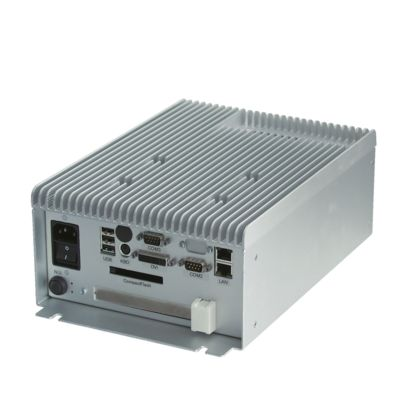
\includegraphics[width=0.9\linewidth]{ImagenesMatriz/IPC.jpg} \\ \hline
		\textbf{15. Registrar datos meteorológicos} & 
		Memoria Flash \par\smallskip 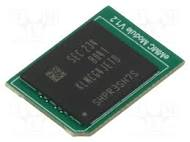
\includegraphics[width=0.7\linewidth]{ImagenesMatriz/MemoriaFLASH.jpg} & 
		MicroSD SPI \par\smallskip 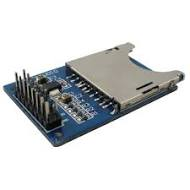
\includegraphics[width=0.7\linewidth]{ImagenesMatriz/ModuloMicroSDSPI.jpg} & 
		EEPROM I2C \par\smallskip 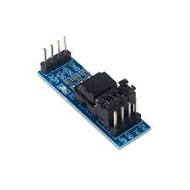
\includegraphics[width=0.7\linewidth]{ImagenesMatriz/MemoriaEEPROMI2C.jpg} \\ \hline
		\textbf{16. Procesar rutas de inspección} & 
		Microcontrolador \par\smallskip 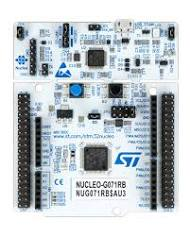
\includegraphics[width=0.7\linewidth]{ImagenesMatriz/Microcontrolador.jpg} & 
		Placa SBC \par\smallskip 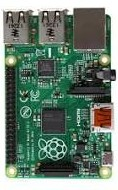
\includegraphics[width=0.7\linewidth]{ImagenesMatriz/SBC.jpg} & 
		Coprocesador GPS \par\smallskip 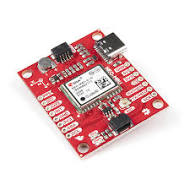
\includegraphics[width=0.9\linewidth]{ImagenesMatriz/ModuloGPSDeadReckoning.jpg} \\ \hline
		\textbf{17. Procesar posición del sistema} & 
		Microcontrolador \par\smallskip 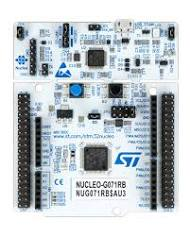
\includegraphics[width=0.7\linewidth]{ImagenesMatriz/Microcontrolador.jpg} & 
		Placa SBC \par\smallskip 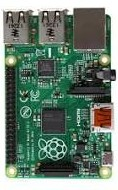
\includegraphics[width=0.7\linewidth]{ImagenesMatriz/SBC.jpg} & 
		Coprocesador GPS\par\smallskip 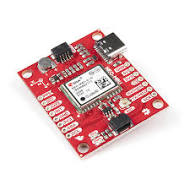
\includegraphics[width=0.9\linewidth]{ImagenesMatriz/ModuloGPSDeadReckoning.jpg} \\ \hline
	\end{xltabular}
\end{center}

\begin{itemize}
	\item \textbf{Funciones de procesamiento lógico y control de variables del sistema:} para el núcleo de estas funciones lógicas y de control, se evaluó la placa SBC, ideal para el procesamiento de datos pesados, cálculos espaciales y operaciones multitarea; el microcontrolador, que ofrece una excelente gestión de lazos cerrados en tiempo real y rutinas secuenciales con bajo consumo energético; y el PLC, que brinda máxima robustez en entornos industriales, pero cuyo tamaño y alta demanda eléctrica limitan su uso en plataformas robóticas móviles.
	
	\item \textbf{Procesar señal de obstáculo:} para la evasión de colisiones se consideró la placa SBC, que posee la capacidad de procesar nubes de puntos o mapas espaciales de forma local; el microcontrolador, útil únicamente si se emplean sensores de umbral simple con baja carga computacional; y una computadora industrial, una solución robusta con la capacidad de procesar algoritmos complejos en tiempo real y comunicarse con protocolos industriales con el PLC.
	
	\item \textbf{Registrar datos meteorológicos:} las opciones de almacenamiento contemplan el módulo MicroSD SPI, una alternativa accesible y de alta capacidad de memoria; la memoria Flash, que es muy rápida y va soldada al circuito impreso, impidiendo su extracción física manual; y la EEPROM I2C, una memoria no volátil de capacidad muy reducida, útil para guardar parámetros de configuración pero puede resultar ineficiente para el registro continuo de bases de datos climáticas.
	
	\item \textbf{Procesar rutas de inspección y Procesar posición del sistema:} para gestionar la ubicación y navegación se analizó la placa SBC, capaz de interpretar mapas complejos y algoritmos avanzados de localización simultánea; el microcontrolador, adecuado para un seguimiento de rutas simples mediante el paso de coordenadas punto a punto; y el coprocesador GPS, un circuito dedicado que se encarga exclusivamente de interpretar las tramas satelitales, liberando a la unidad central de la carga matemática de dichos cálculos espaciales.
\end{itemize}
% --- Tabla de Control (Software) ---
\begin{center}
	\footnotesize
	\begin{xltabular}{\textwidth}{|p{3.5cm}|>{\centering\arraybackslash}X|>{\centering\arraybackslash}X|>{\centering\arraybackslash}X|}
		\caption{Matriz Morfológica del Dominio de Control (Software).}
		\label{tab:matriz_control_sw} \\
		\hline
		\rowcolor[HTML]{D9E1F2} 
		\textbf{Función Parcial} & \textbf{Solución 1} & \textbf{Solución 2} & \textbf{Solución 3} \\ \hline
		\endfirsthead
		\multicolumn{4}{c}%
		{{\bfseries \tablename\ \thetable{} -- Continuación de la página anterior}} \\
		\hline
		\rowcolor[HTML]{D9E1F2} 
		\textbf{Función Parcial} & \textbf{Solución 1} & \textbf{Solución 2} & \textbf{Solución 3} \\ \hline
		\endhead
		\hline
		\endfoot
		\hline
		\endlastfoot
		% --- INICIO BLOQUE DE 8 FILAS ---
		\textbf{1. Procesar datos meteorológicos} & 
		\multirow{8}{=}{\centering Look-up table \par\vspace{0.2cm} 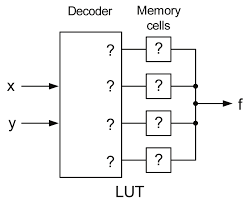
\includegraphics[width=\linewidth]{ImagenesMatriz/LookUpTables.png}} & 
		\multirow{8}{=}{\centering Algoritmo por ecuación \par\vspace{0.2cm} 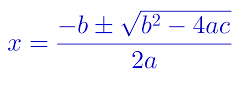
\includegraphics[width=0.8\linewidth]{ImagenesMatriz/AlgoritmoEcuacion.png}} & 
		\multirow{8}{=}{\centering Algoritmo de promedio \par\vspace{0.2cm} 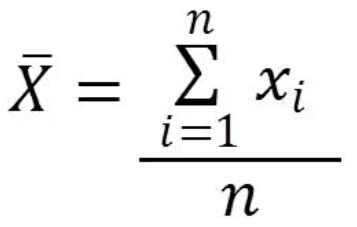
\includegraphics[width=\linewidth]{ImagenesMatriz/AlgoritmoPromedio.png}} \\ \cline{1-1}
		\textbf{2. Procesar temperatura del gestionador} & & & \\ \cline{1-1}
		\textbf{3. Procesar nivel energía del gestionador} & & & \\ \cline{1-1}
		\textbf{4. Procesar estado energía del gestionador} & & & \\ \cline{1-1}
		\textbf{5. Procesar velocidad de traslación} & & & \\ \cline{1-1}
		\textbf{6. Procesar orientación de plataforma} & & & \\ \cline{1-1}
		\textbf{7. Procesar posición de plataforma} & & & \\ \cline{1-1}
		\textbf{8. Controlar estado energía del gestionador} & & & \\ \hline
		\textbf{9. Controlar movimiento de traslación} \vspace{1cm}& 
		\multirow{3}{=}{\centering Control SMC \par\vspace{0.2cm} 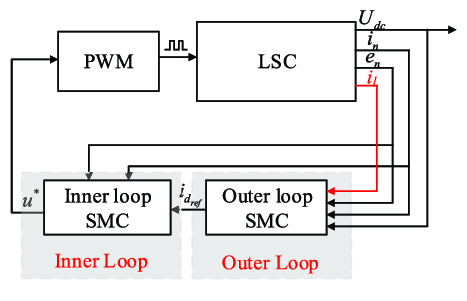
\includegraphics[width=\linewidth]{ImagenesMatriz/ControlSMC.png}} & 
		\multirow{3}{=}{\centering Control PID \par\vspace{0.2cm} 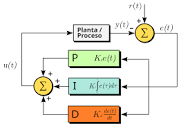
\includegraphics[width=\linewidth]{ImagenesMatriz/ControlPID.png}} & 
		\multirow{3}{=}{\centering Lógica Difusa \par\vspace{0.2cm} 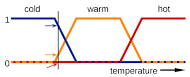
\includegraphics[width=\linewidth]{ImagenesMatriz/LogicaDifusa.png}} \\ \cline{1-1}
		\textbf{10. Controlar movimiento de orientación de plataforma} & & & \\ \cline{1-1}
		\textbf{11. Controlar posicionamiento de plataforma} & & & \\ \hline
		% --- FILAS INDIVIDUALES ---
		\textbf{12. Procesar dirección de traslación} & 
		Controlador Stanley paralelo \par\smallskip 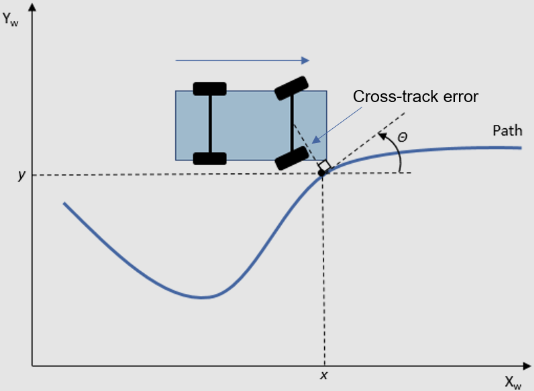
\includegraphics[width=\linewidth]{ImagenesMatriz/StanleyParalelo.png} & 
		Algoritmo Pure Pursuit \par\smallskip 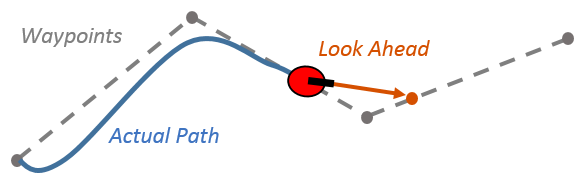
\includegraphics[width=\linewidth]{ImagenesMatriz/PurePursuit.png} & 
		Algoritmo Vector Pursuit\par\smallskip 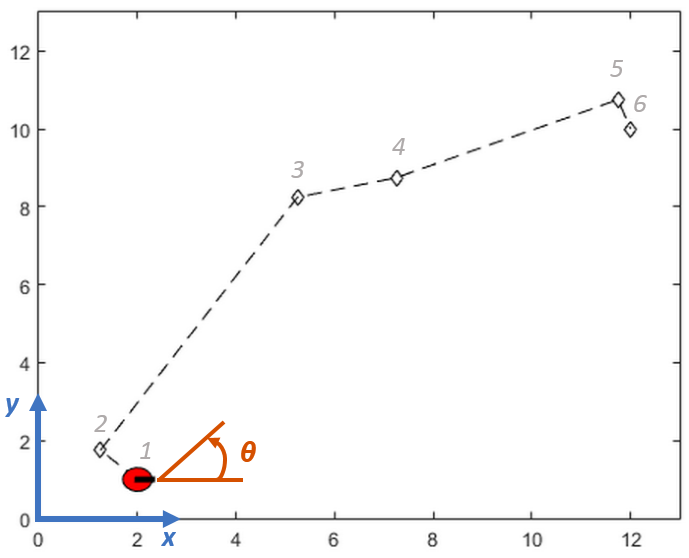
\includegraphics[width=\linewidth]{ImagenesMatriz/VectorPursuit.png} \\ \hline
		\textbf{13. Procesar señal de obstáculo} & 
		Comparación por umbrales y ventanas de tiempo \par\smallskip 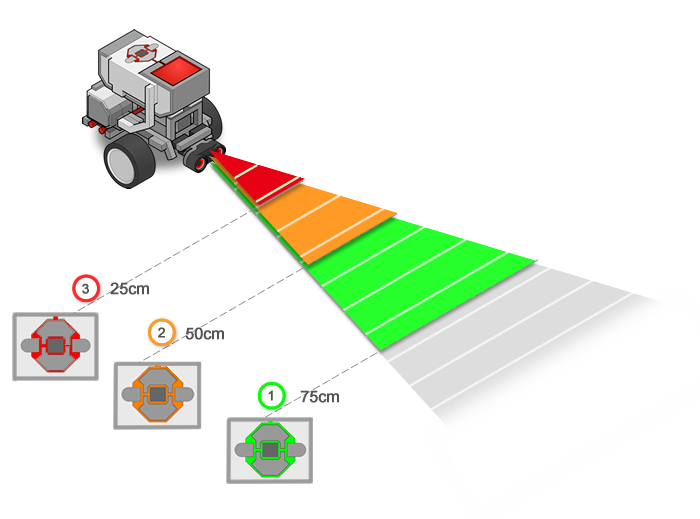
\includegraphics[width=\linewidth]{ImagenesMatriz/Thresholding.png} & 
		Flujo óptico \par\smallskip 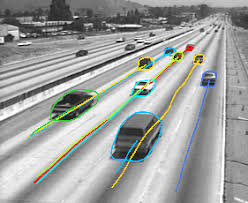
\includegraphics[width=\linewidth]{ImagenesMatriz/OpticalFlow.jpg} & 
		Agrupamiento y segmentación \par\smallskip 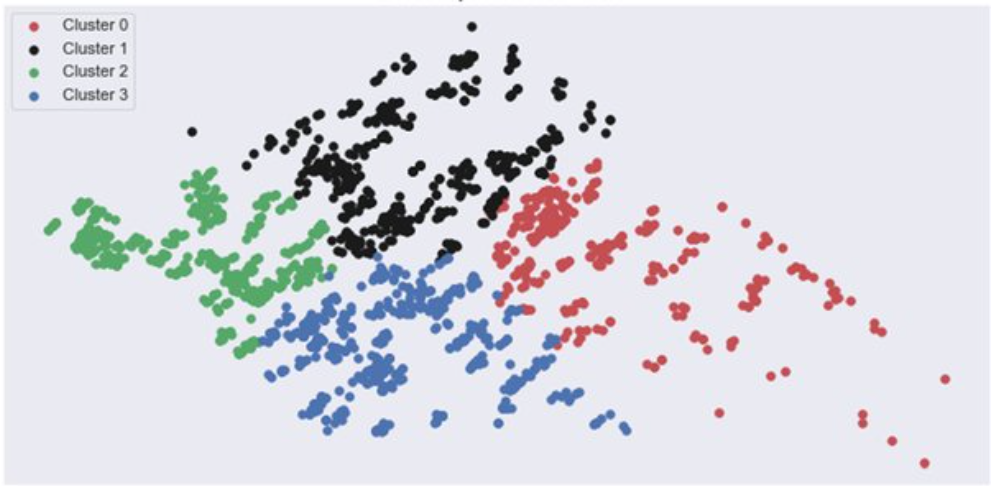
\includegraphics[width=\linewidth]{ImagenesMatriz/AgrupamientoSegmentacion.png} \\ \hline
		\textbf{14. Registrar datos meteorológicos} & 
		Buffer de almacenamiento asíncrono \par\smallskip 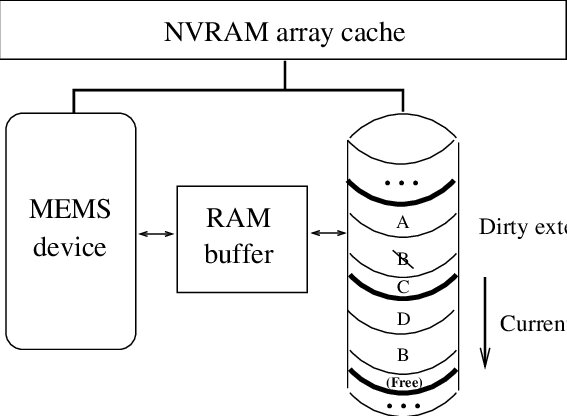
\includegraphics[width=\linewidth]{ImagenesMatriz/AsyncMemoria.jpg} & 
		Acceso directo a sistemas de archivos embebidos \par\smallskip 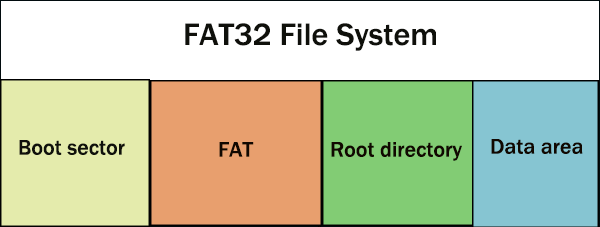
\includegraphics[width=\linewidth]{ImagenesMatriz/FAT32.png} & 
		Motores de data bases \par\smallskip 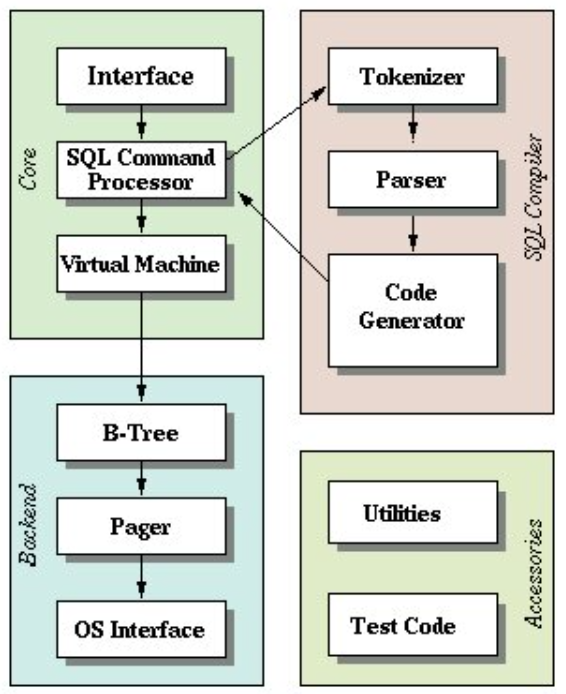
\includegraphics[width=\linewidth]{ImagenesMatriz/SQLite.png} \\ \hline
		\textbf{15. Procesar rutas de inspección} \vspace{1.5cm} & 
		\multirow{2}{=}{\centering A - Navigation por mapas de nodos \par\smallskip 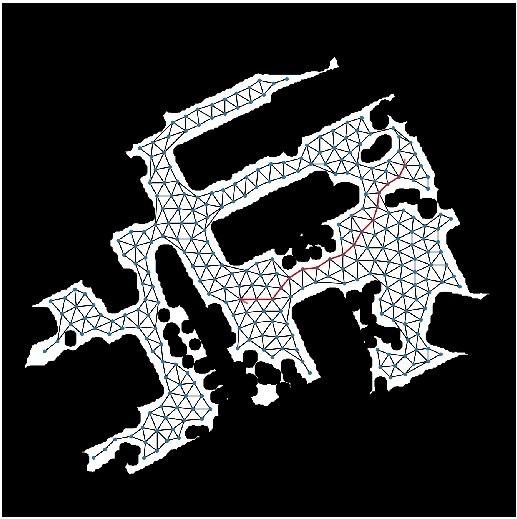
\includegraphics[width=\linewidth]{ImagenesMatriz/RoadmapNodes.jpg}} & 
		\multirow{2}{=}{\centering B - Navegación por histograma de campo vectorial\par\smallskip 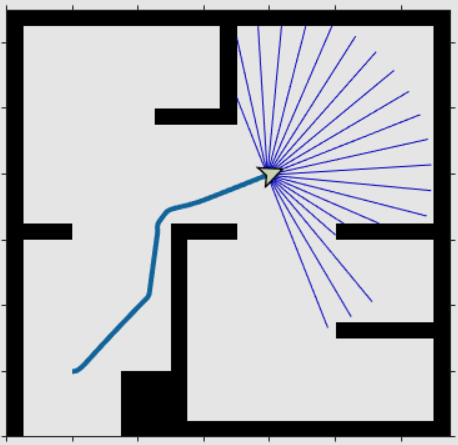
\includegraphics[width=\linewidth]{ImagenesMatriz/VectorFieldNav.png}} & 
		\multirow{2}{=}{\centering C - Navegación por mapas de costo\par\smallskip 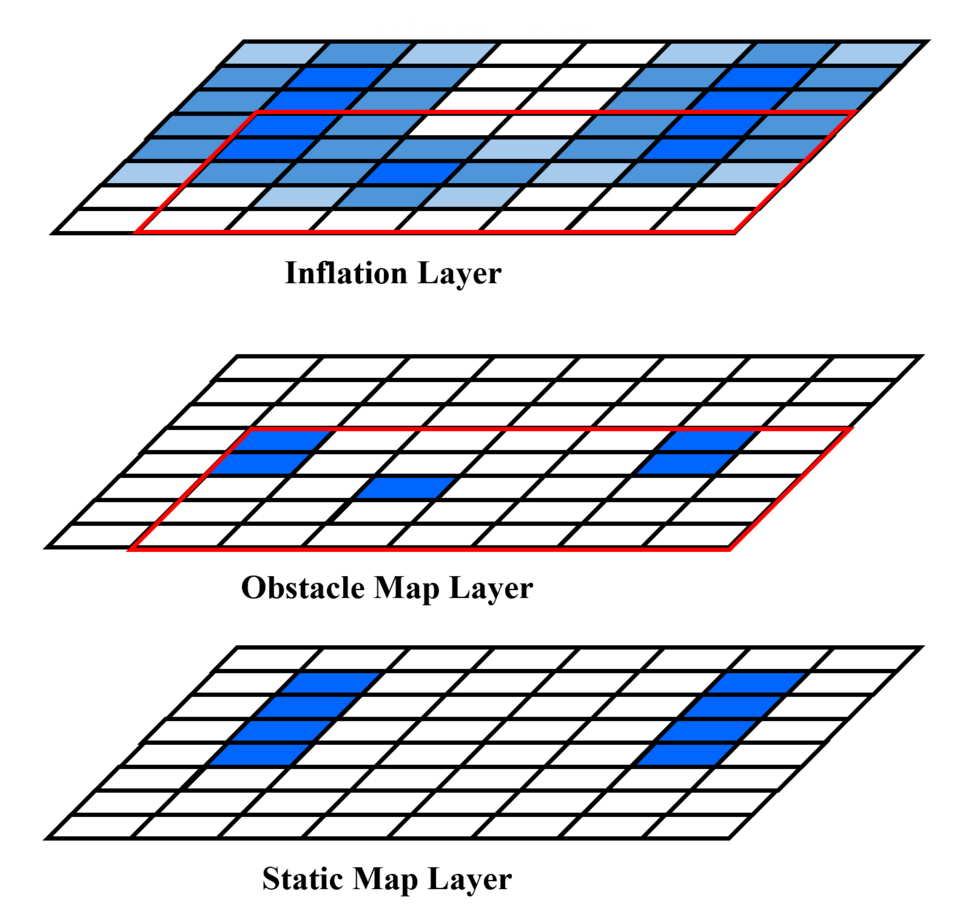
\includegraphics[width=\linewidth]{ImagenesMatriz/Costmap.png}} \\ \cline{1-1}
		\textbf{16. Procesar posición del sistema} \vspace{1.5cm} & & & \\ \hline
	\end{xltabular}
\end{center}

\begin{itemize}
	\item \textbf{Funciones de procesamiento lógico de señales y evaluación del estado general:} para el procesamiento lógico de las señales y la evaluación del estado general, se evaluó el algoritmo por ecuación, que ofrece una conversión matemática exacta pero puede demandar mayor tiempo de procesamiento en el microcontrolador; la look-up table (tabla de búsqueda), que garantiza una ejecución muy rápida al precalcular los valores a costa de ocupar mayor espacio en la memoria; y el algoritmo de promedio, una opción simple que ayuda a filtrar el ruido eléctrico de las lecturas continuas, aunque puede presentar cierto retraso temporal frente a cambios dinámicos rápidos.
	
	\item \textbf{Controlar movimiento de traslación, Controlar movimiento de orientación de plataforma y Controlar posicionamiento de plataforma :} para los lazos de control de los actuadores físicos, se consideró el control PID, que representa el estándar de la industria por su simplicidad y fiabilidad para mantener posiciones o velocidades estables; la lógica difusa, útil para manejar las no linealidades mecánicas mediante reglas lógicas sin requerir un modelo matemático exacto, pero cuya sintonización es compleja; y el control SMC, que destaca por su altísima robustez frente a perturbaciones externas o irregularidades del terreno, aunque puede generar un esfuerzo de control discontinuo y desgaste mecánico prematuro.
	
	\item \textbf{Procesar dirección de traslación:} para guiar el desplazamiento del vehículo, se analizó el algoritmo Pure Pursuit, un método geométrico de seguimiento de ruta sencillo y confiable, pero que tiende a recortar las curvas si la distancia de visión no se ajusta correctamente; el algoritmo Vector Pursuit, que mejora la precisión geométrica al considerar tanto la posición como la orientación del objetivo a alcanzar; y el controlador Stanley paralelo, el cual minimiza eficazmente el error lateral respecto a la trayectoria deseada y se adapta de forma óptima a las variaciones de velocidad del vehículo sobre el terreno.
	
	\item \textbf{Procesar señal de obstáculo:} para la detección y evasión de elementos en la vía, se evaluó la comparación por umbrales y ventanas de tiempo, que exige una carga computacional mínima pero es susceptible a generar falsos positivos por ruido; el agrupamiento y segmentación, ideal para procesar nubes de puntos espaciales separando eficazmente el suelo llano de los obstáculos reales con alta fiabilidad; y el flujo óptico, que detecta el movimiento relativo mediante secuencias de imágenes de cámara, aunque su eficacia disminuye drásticamente en entornos con iluminación variable o alto nivel de polvo.
	
	\item \textbf{Registrar datos meteorológicos:} para el resguardo de la información climática, se propuso el acceso directo a sistemas de archivos embebidos, que permite una escritura secuencial simple pero puede bloquear temporalmente el procesador principal; los motores de bases de datos, que estructuran la información para facilitar consultas complejas y búsquedas a cambio de una alta exigencia de memoria RAM; y el buffer de almacenamiento asíncrono, que garantiza que los datos se recopilen y guarden en segundo plano sin interrumpir los tiempos de ejecución de los ciclos críticos de control del robot.
	
	\item \textbf{Procesar rutas de inspección y Procesar posición del sistema:} para planificar y seguir el recorrido dentro del parque fotovoltaico, se consideró la navegación por mapas de nodos, que requiere escasa memoria al estructurar la planta solar simplemente como un grafo de puntos secuenciales a visitar; la navegación por mapas de costo, que permite representar áreas seguras, zonas de riesgo y obstáculos como gradientes para un desplazamiento mucho más seguro; y la navegación por histograma de campo vectorial, excelente para calcular trayectorias y evadir obstáculos locales de forma fluida y en tiempo real.
\end{itemize}

\subsection{Dominio de Comunicación}
% Espacio para tabla de Comunicación
\begin{center}
	\footnotesize
	\begin{xltabular}{\textwidth}{|p{3.5cm}|>{\raggedright\arraybackslash}X|>{\raggedright\arraybackslash}X|>{\raggedright\arraybackslash}X|}
		\caption{Matriz Morfológica del Dominio de Comunicación.}
		\label{tab:matriz_comunicacion} \\
		\hline
		\rowcolor[HTML]{D9E1F2} 
		\textbf{Función Parcial} & \textbf{Solución 1} & \textbf{Solución 2} & \textbf{Solución 3} \\ \hline
		\endfirsthead
		\multicolumn{4}{c}%
		{{\bfseries \tablename\ \thetable{} -- Continuación de la página anterior}} \\
		\hline
		\rowcolor[HTML]{D9E1F2} 
		\textbf{Función Parcial} & \textbf{Solución 1} & \textbf{Solución 2} & \textbf{Solución 3} \\ \hline
		\endhead
		\hline
		\endfoot
		\hline
		\endlastfoot
		% --- INICIO BLOQUE 1-2 ---
		\textbf{1. Procesar señal GPS} \vspace{0.8cm} & 
		\multirow{2}{=}{ Trilaterización \par\smallskip 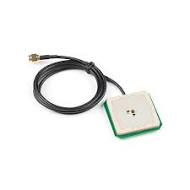
\includegraphics[width=0.7\linewidth]{ImagenesMatriz/AntenaGNSS.jpg}} & 
		\multirow{2}{=}{ Trilaterización con Dead Reckoning \par\smallskip 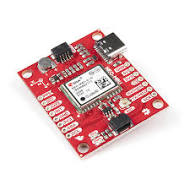
\includegraphics[width=0.7\linewidth]{ImagenesMatriz/ModuloGPSDeadReckoning.jpg}} & 
		\multirow{2}{=}{ Medición de fase de onda \par\smallskip 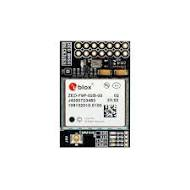
\includegraphics[width=0.7\linewidth]{ImagenesMatriz/ModuloFasePortadora.jpg}} \\ \cline{1-1}
		\textbf{2. Procesar señal de mando} \vspace{0.8cm} & & & \\ \hline
		% --- FIN BLOQUE 1-2 ---
		% --- INICIO BLOQUE 3-4 ---
		\textbf{3. Transmitir estado de telemetría} \vspace{0.8cm} & 
		\multirow{2}{=}{Protocolo MQTT +Wi-Fi\par\smallskip 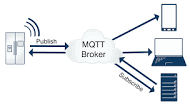
\includegraphics[width=\linewidth]{ImagenesMatriz/ProtocoloMQTT.png}} & 
		\multirow{2}{=}{Módulo LoRa \par\smallskip 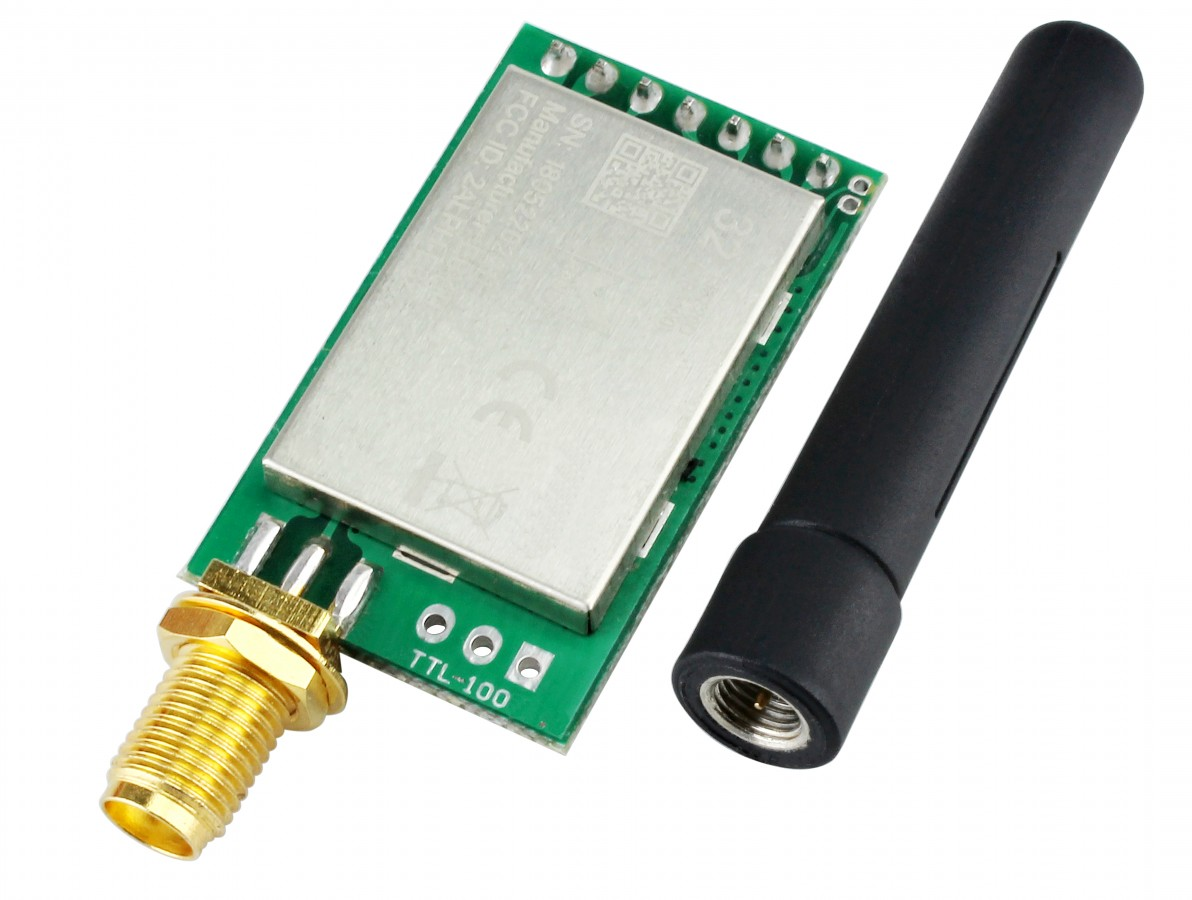
\includegraphics[width=0.7\linewidth]{ImagenesMatriz/ModuloLoRa.jpg}} & 
		\multirow{2}{=}{Celular LTE-M \par\smallskip 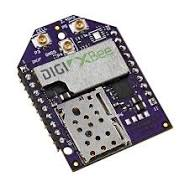
\includegraphics[width=0.7\linewidth]{ImagenesMatriz/CelularLTEM.jpg}} \\ \cline{1-1}
		\textbf{4. Transmitir datos meteorológicos} \vspace{0.2cm}& & & \\ \hline
		% --- FIN BLOQUE 3-4 ---
	\end{xltabular}
\end{center}

\begin{itemize}
	\item \textbf{Procesar señal GPS y Procesar señal de mando:} para el cálculo de la ubicación y el procesamiento de instrucciones se evaluó la trilateración, un método de posicionamiento estándar y económico basado en la distancia a los satélites, aunque vulnerable a la pérdida de conexión; la medición de fase de onda (tipo RTK), que otorga una alta precisión centimétrica pero requiere el uso de una estación base y mayor capacidad de procesamiento; y la trilateración con Dead Reckoning, que combina los datos satelitales con la odometría interna del vehículo para mantener la estimación exacta de la posición incluso cuando la señal satelital se bloquea al transitar bajo los paneles solares.
	
	\item \textbf{Transmitir estado de telemetría y Transmitir datos meteorológicos:} para la emisión de la información y alertas hacia el exterior se analizó el módulo LoRa, que permite la transmisión de datos a largas distancias con un consumo energético mínimo, siendo ideal para las grandes extensiones de terreno de las plantas solares; el celular LTE-M, que ofrece una conexión directa a la nube con un mayor ancho de banda, pero depende de la disponibilidad y estabilidad de la cobertura de la red operadora local; y la combinación del protocolo MQTT + Wi-Fi, que garantiza una alta velocidad para la transferencia de paquetes, pero cuyo alcance limitado exigiría instalar una costosa red de múltiples puntos de acceso a lo largo de todo el terreno.
\end{itemize}

\subsection{Dominio de Interfaz}
% Espacio para tabla de Interfaz

\begin{center}
	\footnotesize
	\begin{xltabular}{\textwidth}{|p{3.5cm}|>{\raggedright\arraybackslash}X|>{\raggedright\arraybackslash}X|>{\raggedright\arraybackslash}X|}
		\caption{Matriz Morfológica del Dominio de Interfaz.}
		\label{tab:matriz_interfaz} \\
		\hline
		\rowcolor[HTML]{D9E1F2} 
		\textbf{Función Parcial} & \textbf{Solución 1} & \textbf{Solución 2} & \textbf{Solución 3} \\ \hline
		\endfirsthead
		\multicolumn{4}{c}%
		{{\bfseries \tablename\ \thetable{} -- Continuación de la página anterior}} \\
		\hline
		\rowcolor[HTML]{D9E1F2} 
		\textbf{Función Parcial} & \textbf{Solución 1} & \textbf{Solución 2} & \textbf{Solución 3} \\ \hline
		\endhead
		\hline
		\endfoot
		\hline
		\endlastfoot
		% --- INICIO BLOQUE 1-4 ---
		\textbf{1. Recibir señal de radiación} & 
		\multirow{4}{=}{Conector circular roscado \par\smallskip 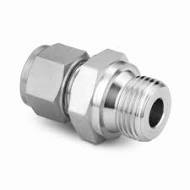
\includegraphics[width=0.8\linewidth]{ImagenesMatriz/ConectorRoscado.jpg}} & 
		\multirow{4}{=}{Borna con resorte interno \par\smallskip 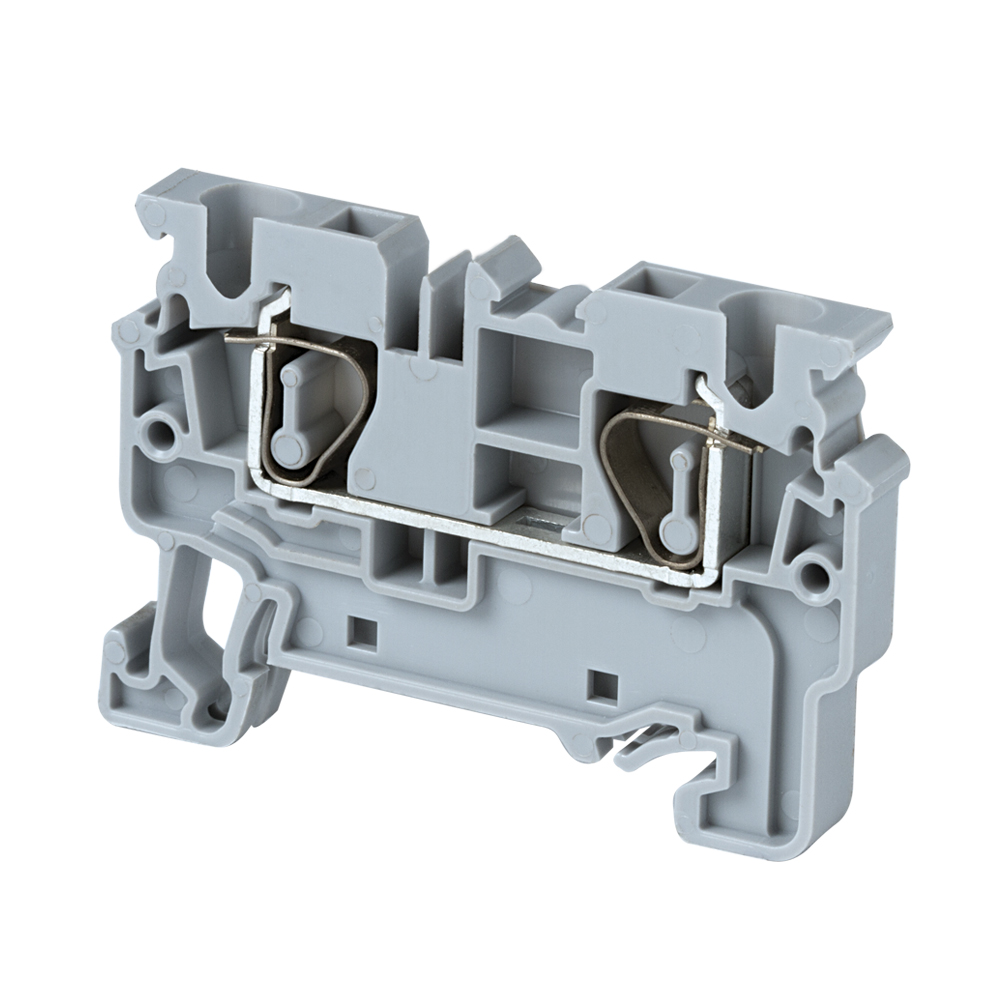
\includegraphics[width=0.8\linewidth]{ImagenesMatriz/BornaResorte.jpg}} & 
		\multirow{4}{=}{Conector Deutsch \par\smallskip 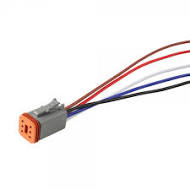
\includegraphics[width=\linewidth]{ImagenesMatriz/ConectorDeutsch.jpg}} \\ \cline{1-1}
		\textbf{2. Recibir señal de temperatura} & & & \\ \cline{1-1}
		\textbf{3. Recibir señal de velocidad viento} & & & \\ \cline{1-1}
		\textbf{4. Recibir señal de humedad} & & & \\ \hline
		% --- FIN BLOQUE 1-4 ---
		% --- INICIO BLOQUE 5-6 ---
		\textbf{5. Mostrar alerta obstáculo} \vspace{1cm}& 
		\multirow{2}{=}{Buzzer \par\smallskip 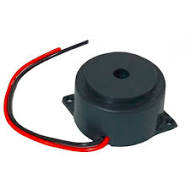
\includegraphics[width=0.8\linewidth]{ImagenesMatriz/Buzzer.jpg}} & 
		\multirow{2}{=}{Pantalla LCD \par\smallskip 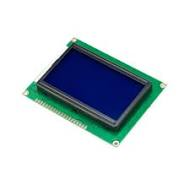
\includegraphics[width=0.8\linewidth]{ImagenesMatriz/PantallaLCD.jpg}} & 
		\multirow{2}{=}{Sirena LED \par\smallskip 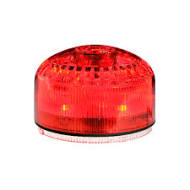
\includegraphics[width=0.8\linewidth]{ImagenesMatriz/SirenaLED.jpg}} \\ \cline{1-1}
		\textbf{6. Mostrar alerta energía} & & & \\ \hline
		% --- FIN BLOQUE 5-6 ---
		
		
		% --- INICIO BLOQUE 7-8 ---
		\textbf{7. Mostrar estado energía} \vspace{1cm}& 
		\multirow{2}{=}{LEDs indicadores \par\smallskip 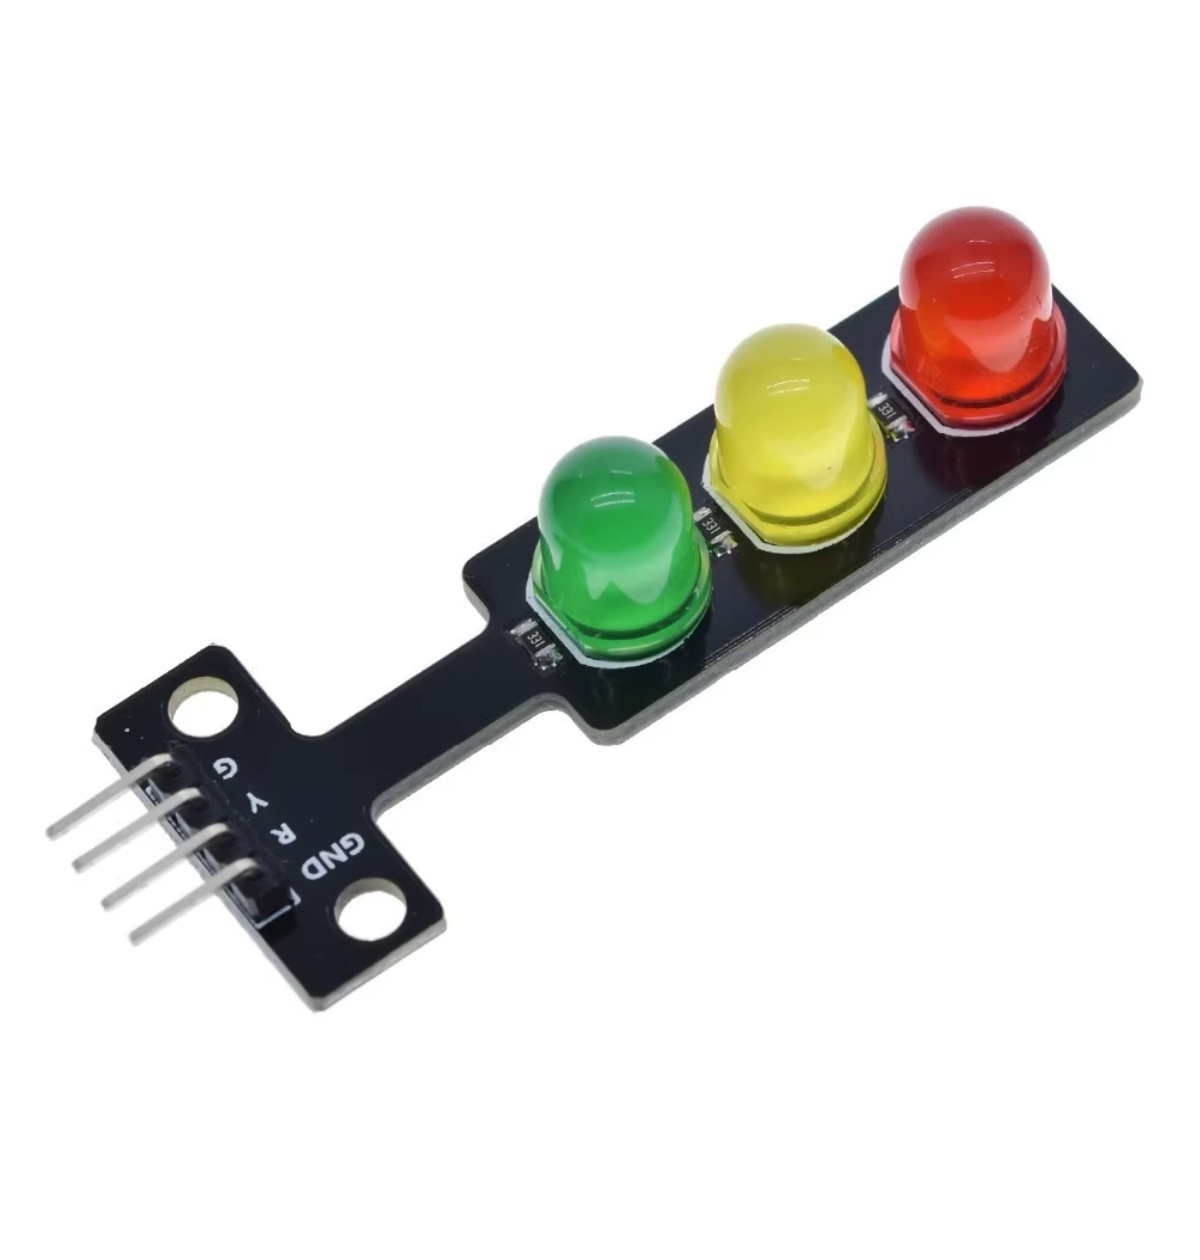
\includegraphics[width=0.8\linewidth]{ImagenesMatriz/LEDIndicador.jpeg}} & 
		\multirow{2}{=}{Pantalla LCD \par\smallskip 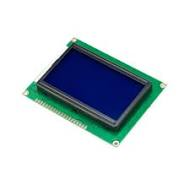
\includegraphics[width=0.8\linewidth]{ImagenesMatriz/PantallaLCD.jpg}} & 
		\multirow{2}{=}{Pantalla HMI \par\smallskip 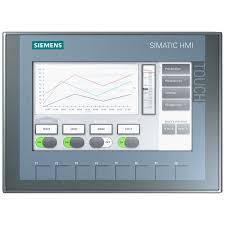
\includegraphics[width=0.8\linewidth]{ImagenesMatriz/PantallaHMI.jpg}} \\ \cline{1-1}
		\textbf{8. Mostrar estado operativo} & & & \\ \hline
		% --- FIN BLOQUE 7-8 ---
	\end{xltabular}
\end{center}

\begin{itemize}
	\item \textbf{Funciones de recepción de señales de instrumentación meteorológica:} para la conexión de los sensores externos se evaluó la borna con resorte interno, que permite un ensamblaje rápido del cableado pero es vulnerable a desconexiones por las continuas vibraciones del robot sobre el terreno; el conector circular roscado, que garantiza un acople industrial firme y con alta protección contra el polvo y la humedad propia del entorno de la planta; y el conector Deutsch, reconocido por su excelente sello hermético en vehículos, pero que exige herramientas especiales de crimpado que dificultan su mantenimiento en campo.
	
	\item \textbf{Mostrar alerta obstáculo y Mostrar alerta energía:} para la emisión de advertencias críticas se consideró el buzzer, que proporciona una alarma sonora inmediata y efectiva con un consumo de energía mínimo para prevenir colisiones; la sirena LED, que entrega un aviso combinado de alta potencia pero resulta sobredimensionada y representa un gasto energético excesivo para el tamaño del vehículo; y la pantalla LCD, que si bien detalla el tipo de error, es ineficiente como mecanismo de alerta rápida ya que requiere que el personal se acerque al equipo para poder leerla.
	
	\item \textbf{Mostrar estado energía y Mostrar estado operativo:} para la supervisión local y directa del sistema se analizó la pantalla LCD, útil para mostrar valores exactos pero propensa a reflejos bajo la luz directa del sol; la pantalla HMI, que ofrece una interacción táctil avanzada a cambio de una mayor fragilidad ante impactos and un alto consumo de las baterías; y los LEDs indicadores, que representan la opción más robusta y eficiente al codificar los estados operativos mediante colores simples, lo que permite una lectura rápida a la distancia prescindiendo de pantallas de alto consumo.
\end{itemize}

\subsection{Dominio de Actuadores}
% Espacio para tabla de Actuadores

\begin{center}
	\footnotesize
	\begin{xltabular}{\textwidth}{|p{3.5cm}|>{\raggedright\arraybackslash}X|>{\raggedright\arraybackslash}X|>{\raggedright\arraybackslash}X|}
		\caption{Matriz Morfológica del Dominio de Actuadores.}
		\label{tab:matriz_actuadores} \\
		\hline
		\rowcolor[HTML]{D9E1F2} 
		\textbf{Función Parcial} & \textbf{Solución 1} & \textbf{Solución 2} & \textbf{Solución 3} \\ \hline
		\endfirsthead
		
		\multicolumn{4}{c}%
		{{\bfseries \tablename\ \thetable{} -- Continuación de la página anterior}} \\
		\hline
		\rowcolor[HTML]{D9E1F2} 
		\textbf{Función Parcial} & \textbf{Solución 1} & \textbf{Solución 2} & \textbf{Solución 3} \\ \hline
		\endhead
		
		\hline
		\endfoot
		
		\hline
		\endlastfoot
		
		\textbf{1. Accionar movimiento de traslación} 
		& Motor de Cubo de Rueda \par\smallskip 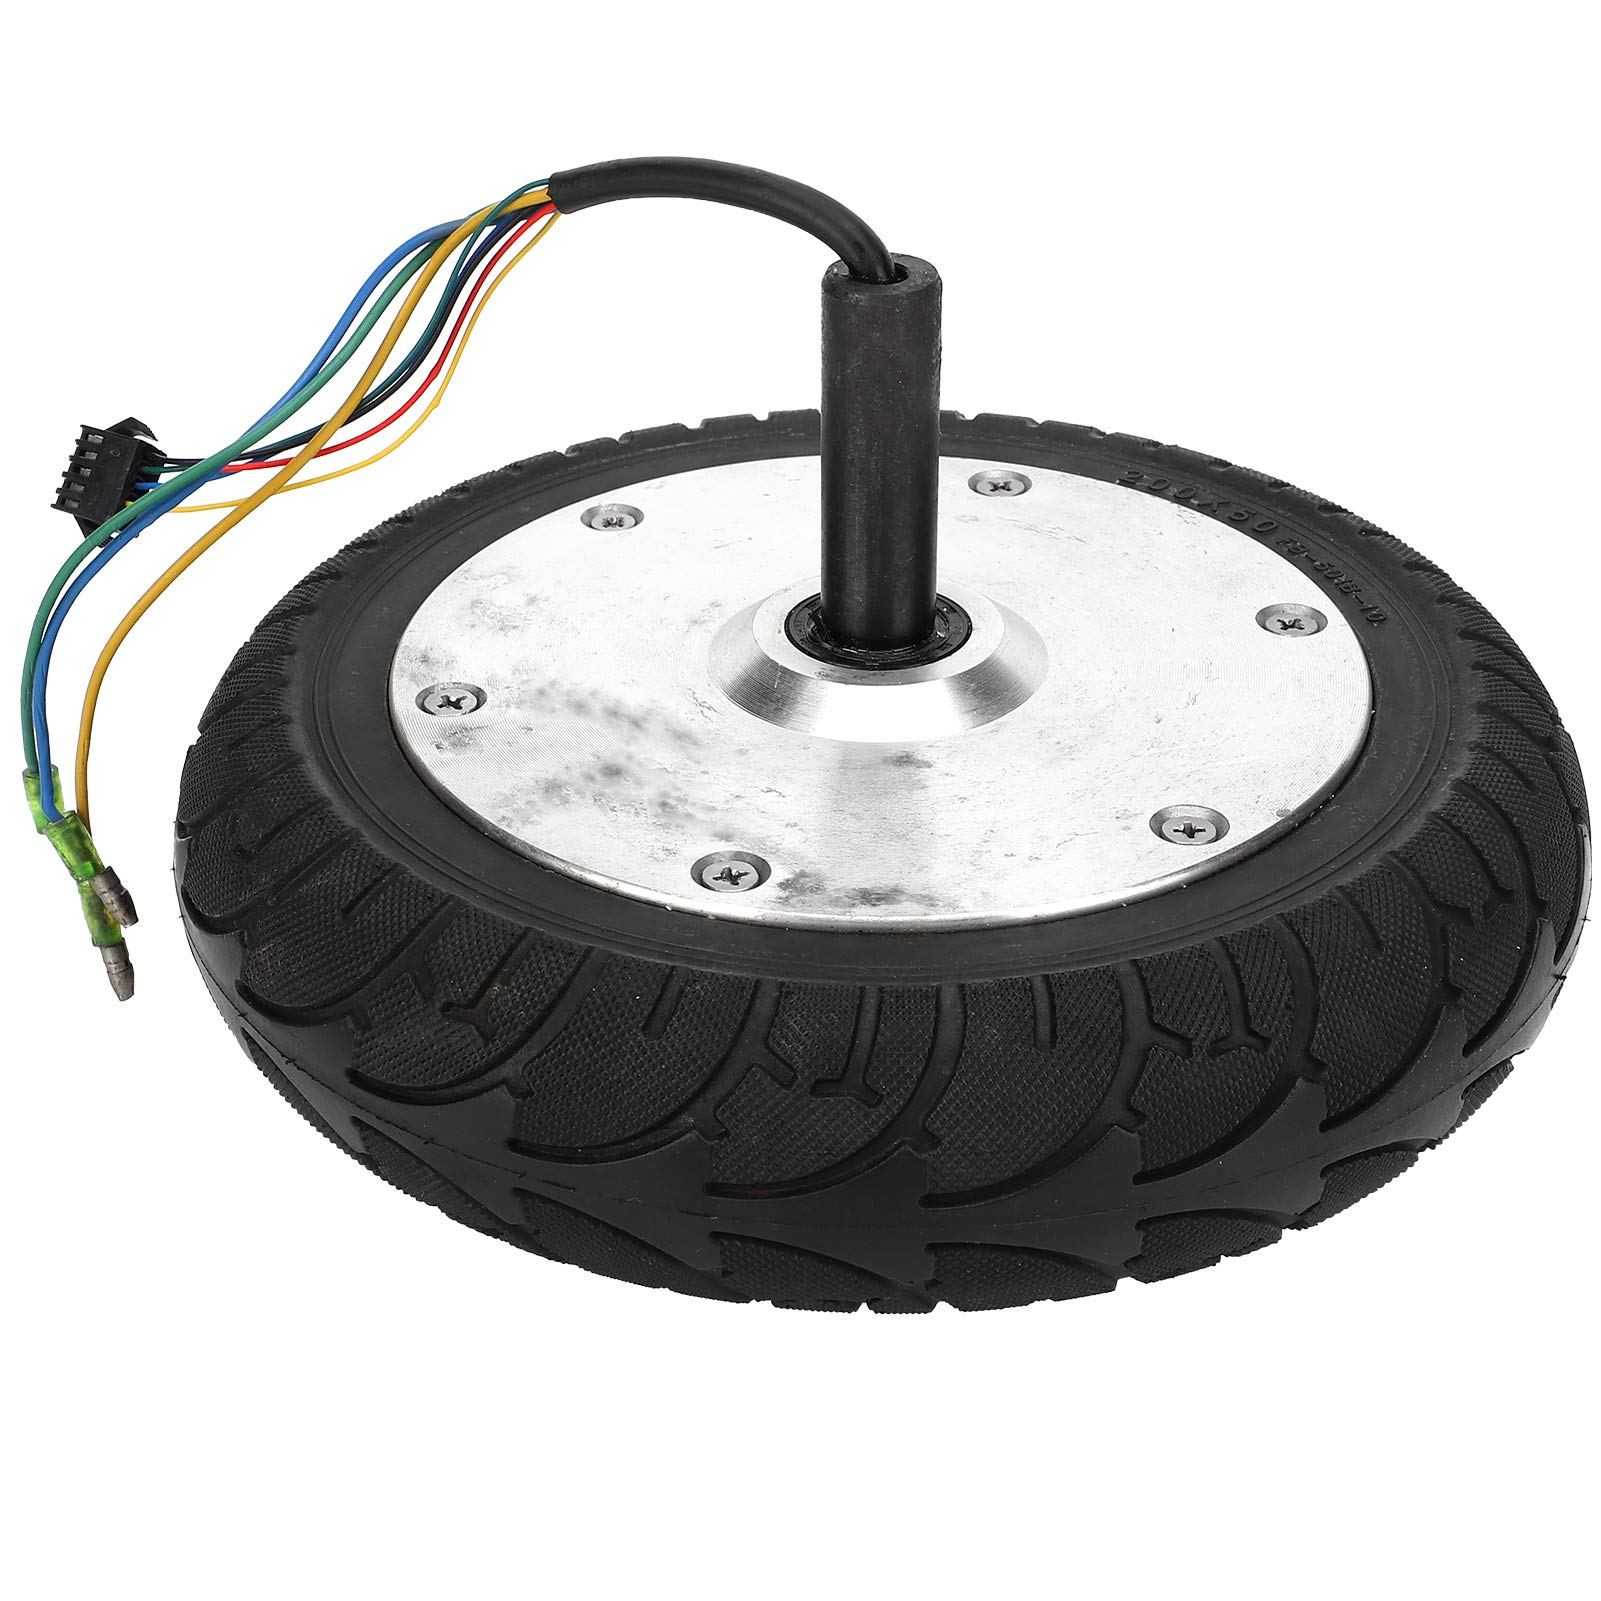
\includegraphics[width=\linewidth]{ImagenesMatriz/MotorCuboDeRueda.jpg} & Servomotor Brushless DC \par\smallskip 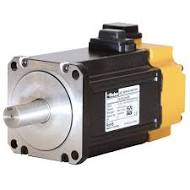
\includegraphics[width=\linewidth]{ImagenesMatriz/ServomotorBrushless.jpg} &  Motorreductor DC  \par\smallskip 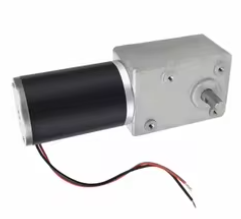
\includegraphics[width=\linewidth]{ImagenesMatriz/MotorreductorDC.png} \\ \hline
		\textbf{2. Accionar orientación de la plataforma} & 
		Microservo digital \par\smallskip 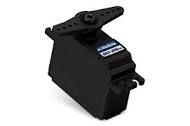
\includegraphics[width=\linewidth]{ImagenesMatriz/Miniservo.jpg}& Servomotor Brushless DC \par\smallskip 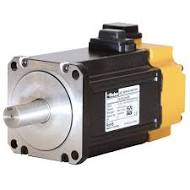
\includegraphics[width=\linewidth]{ImagenesMatriz/ServomotorBrushless.jpg}& 	Motor paso a paso NEMA \par\smallskip 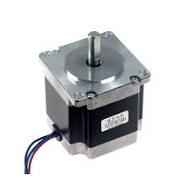
\includegraphics[width=\linewidth]{ImagenesMatriz/MotorNEMA.jpg}\\ \hline
		\textbf{3. Accionar posición de la plataforma} &
		Actuador lineal \par\smallskip 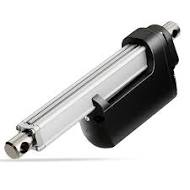
\includegraphics[width=\linewidth]{ImagenesMatriz/ActuadorLineal.jpg} & Servomotor Brushless DC \par\smallskip 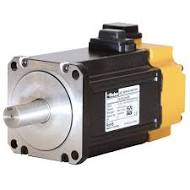
\includegraphics[width=\linewidth]{ImagenesMatriz/ServomotorBrushless.jpg}& Actuador lineal \par\smallskip 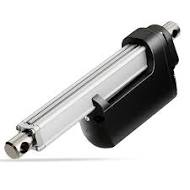
\includegraphics[width=\linewidth]{ImagenesMatriz/ActuadorLineal.jpg}\\ \hline
		
	\end{xltabular}
\end{center}


\begin{itemize}
	\item \textbf{Accionar movimiento de traslación:} para la tracción principal del vehículo sobre el terreno, se evaluó el motor paso a paso NEMA, que ofrece un alto torque a bajas velocidades y un avance preciso, aunque con un consumo energético constante y elevado; el servomotor Brushless DC, que brinda una alta eficiencia, vida útil prolongada y control exacto en lazo cerrado para la navegación, pero con mayor costo y complejidad de implementación; y el motor DC estándar, que representa una opción económica y de control sencillo, pero es susceptible a un mayor desgaste mecánico y posee menor precisión para sortear las irregularidades del suelo.
	
	\item \textbf{Accionar orientación de la plataforma:} para el ajuste del ángulo de los instrumentos de medición climática, se consideró el motor paso a paso NEMA, que asegura una excelente retención estática y precisión para mantener la inclinación deseada frente a las vibraciones del entorno; el servomotor Brushless DC, que proporciona un control angular de gran exactitud pero resulta técnica y económicamente sobredimensionado para sostener una carga estática; y el microservo digital, una alternativa muy compacta y de control directo, pero cuya transmisión y engranajes internos pueden ser vulnerables a daños mecánicos bajo los esfuerzos continuos de la plataforma.
	
	\item \textbf{Accionar posición de la plataforma:} Se evaluó el servomotor Brushless DC, que proporciona alta precisión pero exige un consumo eléctrico continuo para mantener la carga estática y el actuador lineal, con una capacidad de ejecutar el movimiento rectilíneo directo y retener mecánicamente la elevación sin consumo de energía constante.

\end{itemize}
\subsection{Dominio Mecánico}
% Espacio para tabla de Mecánico
\begin{center}
	\footnotesize
	\begin{xltabular}{\textwidth}{|p{3.5cm}|>{\raggedright\arraybackslash}X|>{\raggedright\arraybackslash}X|>{\raggedright\arraybackslash}X|}
		\caption{Matriz Morfológica del Dominio Mecánico.}
		\label{tab:matriz_mecanico} \\
		\hline
		\rowcolor[HTML]{D9E1F2} 
		\textbf{Función Parcial} & \textbf{Solución 1} & \textbf{Solución 2} & \textbf{Solución 3} \\ \hline
		\endfirsthead
		\multicolumn{4}{c}%
		{{\bfseries \tablename\ \thetable{} -- Continuación de la página anterior}} \\
		\hline
		\rowcolor[HTML]{D9E1F2} 
		\textbf{Función Parcial} & \textbf{Solución 1} & \textbf{Solución 2} & \textbf{Solución 3} \\ \hline
		\endhead
		\hline
		\endfoot
		\hline
		\endlastfoot
		% --- INICIO BLOQUE 1-2 ---
		\textbf{1. Soportar plataforma de medición} \vspace{1cm}& 
		\multirow{2}{=}{Piezas de MDF \par\smallskip 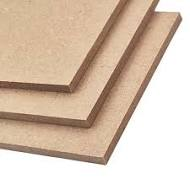
\includegraphics[width=0.8\linewidth]{ImagenesMatriz/PiezasMDF.jpg}} & 
		\multirow{2}{=}{Perfil V-Slot \par\smallskip 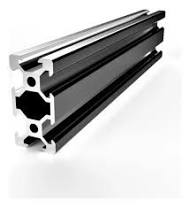
\includegraphics[width=0.8\linewidth]{ImagenesMatriz/Vslot.jpg}} & 
		\multirow{2}{=}{Chapas de Acero \par\smallskip 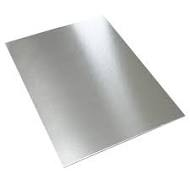
\includegraphics[width=0.8\linewidth]{ImagenesMatriz/ChapaAcero.jpg}} \\ \cline{1-1}
		\textbf{2. Soportar componentes} & & & \\ \hline
		\textbf{3. Proteger componentes} \vspace{1cm}& 
		\multirow{3}{=}{Carcasa impresa en 3D \par\smallskip 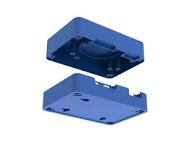
\includegraphics[width=0.8\linewidth]{ImagenesMatriz/Carcasa3D.jpg}} & 
		\multirow{3}{=}{Caja de chapa de aluminio \par\smallskip 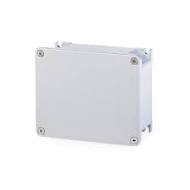
\includegraphics[width=0.8\linewidth]{ImagenesMatriz/CajaChapaAluminio.jpg}} & 
		\multirow{3}{=}{Caja de acero inoxidable \par\smallskip 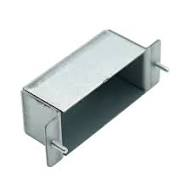
\includegraphics[width=0.8\linewidth]{ImagenesMatriz/CajaChapaAcero.jpg}} \\ \cline{1-1}
		\textbf{4. Alojar gestionador} & & & \\ \cline{1-1}
		\textbf{5. Alojar memoria externa} & & & \\ \hline
		\textbf{6. Generar movimiento de traslación} & 
		Ruedas onmidireccionales \par\smallskip 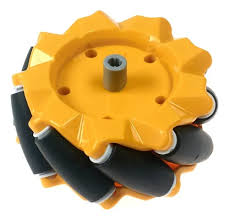
\includegraphics[width=\linewidth]{ImagenesMatriz/RuedaOnmidireccional.jpg} & 
		Tracción diferencial (4 ruedas) \par\smallskip 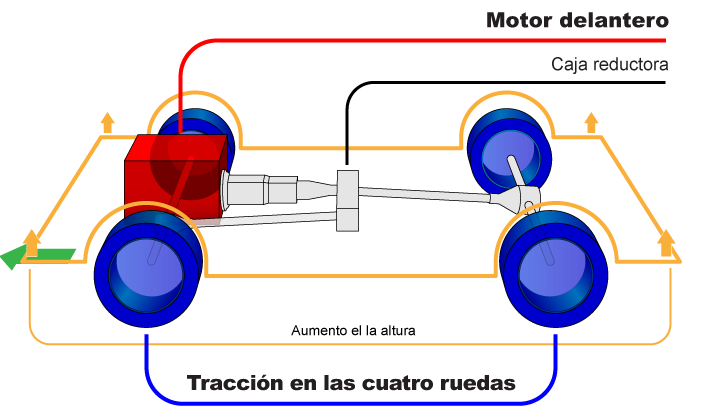
\includegraphics[width=\linewidth]{ImagenesMatriz/RuedasTraccionDiferencial.png} & 
		Ruedas con tracción de oruga \par\smallskip 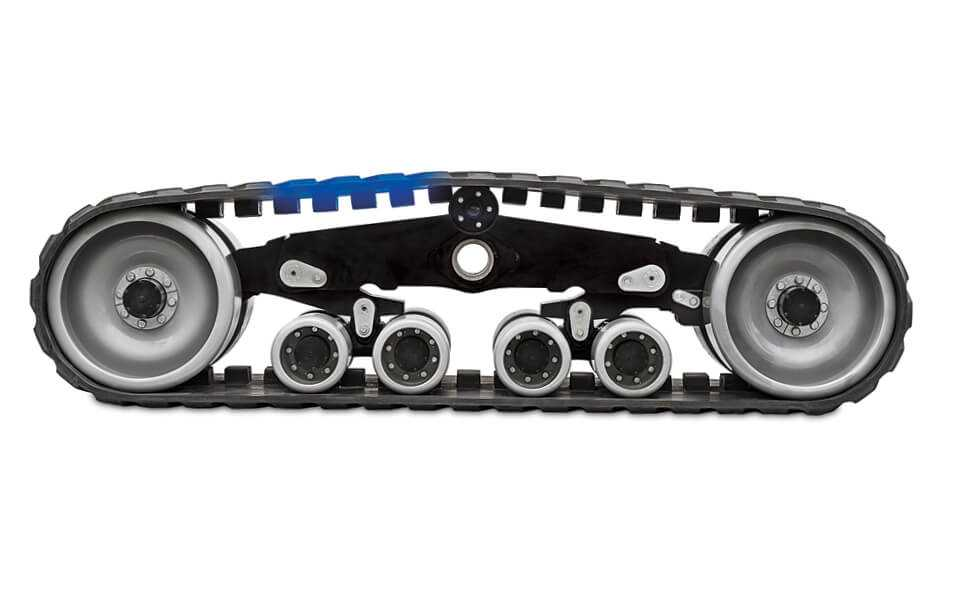
\includegraphics[width=\linewidth]{ImagenesMatriz/RuedasTraccionOruga.jpg} \\ \hline
		\textbf{7. Orientar plataforma} & 
		Eje acoplado a motor \par\smallskip 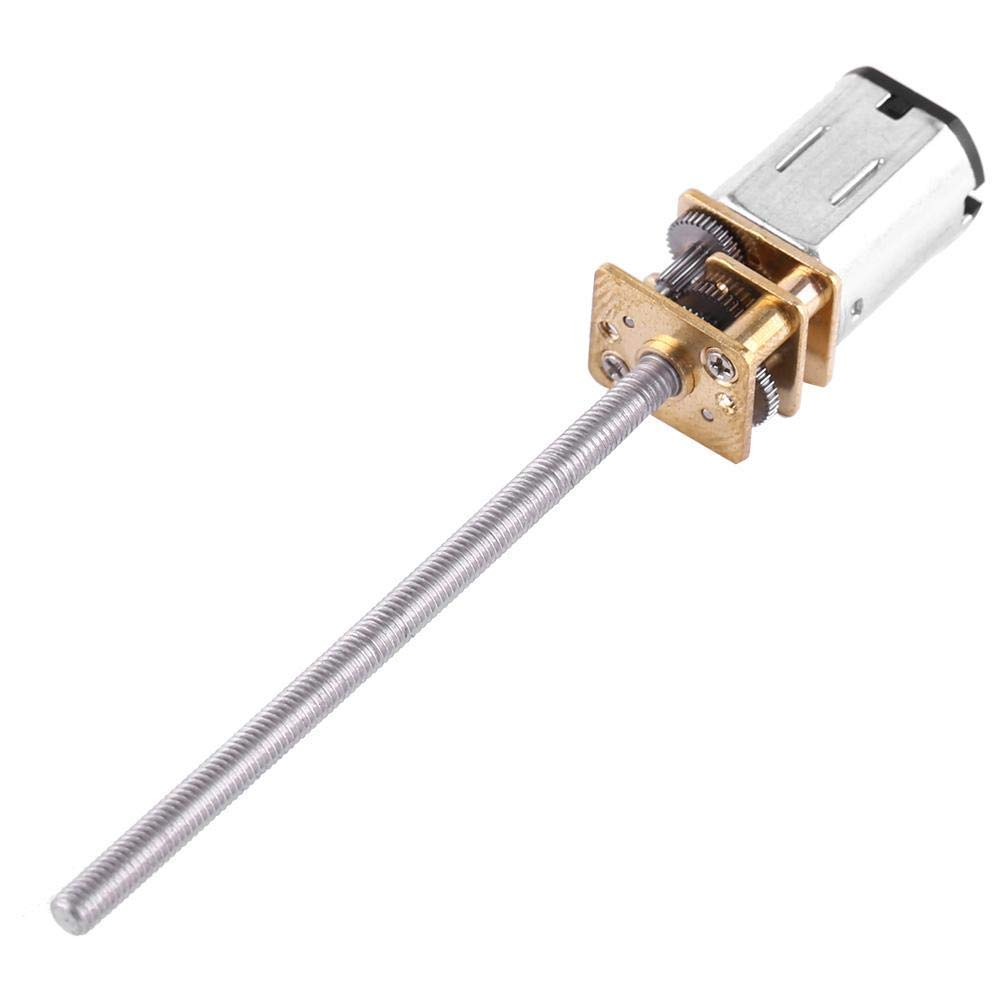
\includegraphics[width=\linewidth]{ImagenesMatriz/MotorEje.jpg}& 
		Mecanismo tornillo sinfin-corona curva \par\smallskip 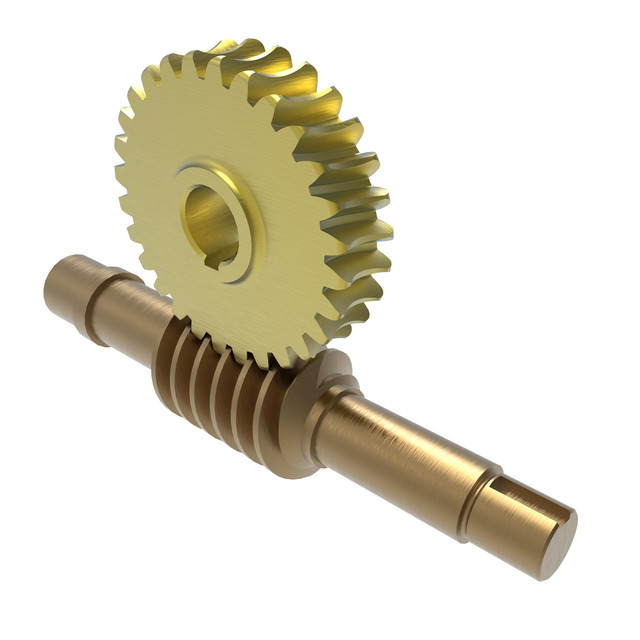
\includegraphics[width=\linewidth]{ImagenesMatriz/TornilloSinFinCorona.jpg}& 
		Transmisión por correa dentada \par\smallskip 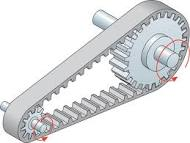
\includegraphics[width=\linewidth]{ImagenesMatriz/TransmisionCorreaDentada.jpg}\\ \hline
		\textbf{8. Posicionar plataforma} & 
		Soporte vertical  \par\smallskip 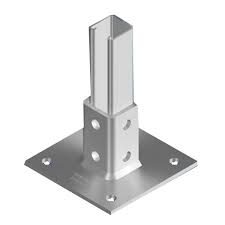
\includegraphics[width=\linewidth]{ImagenesMatriz/SoporteVertical.jpg}& 
		Plataforma elevadora de tijera \par\smallskip 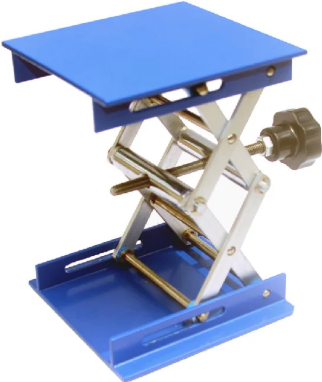
\includegraphics[width=\linewidth]{ImagenesMatriz/TijeraElevacion.png}& 
		Elevacion por articulación telescópica\par\smallskip 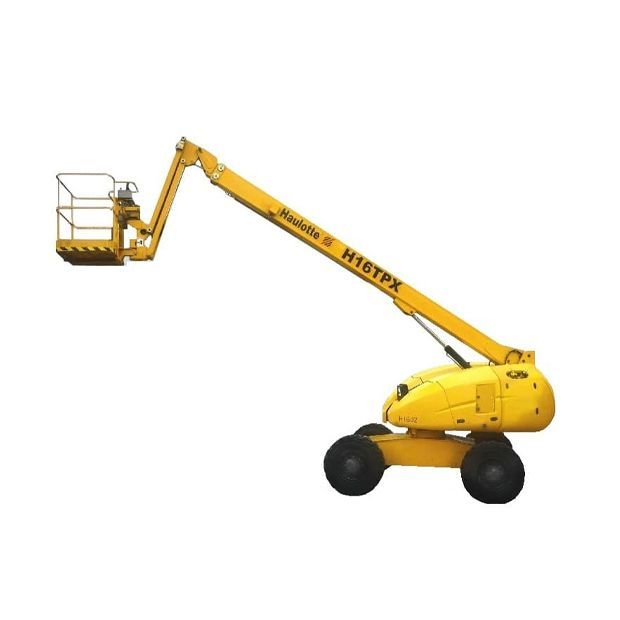
\includegraphics[width=\linewidth]{ImagenesMatriz/PlataformaTelescopica.jpg}\\ \hline
	\end{xltabular}
\end{center}

\begin{itemize}
	\item \textbf{Soportar plataforma de medición y Soportar componentes:} para conformar la estructura base, se evaluó el perfil V-Slot de aluminio, que ofrece una excelente relación resistencia-peso y gran modularidad para el ensamblaje; las chapas de acero, que brindan máxima rigidez estructural pero penalizan drásticamente el peso total del vehículo limitando su autonomía; y las piezas de MDF, una opción económica para prototipado rápido, pero mecánicamente frágil y vulnerable a la humedad del entorno exterior.
	
	\item \textbf{Proteger componentes, Alojar gestionador y Alojar memoria externa:} para el resguardo de la electrónica y módulos, se analizó la caja de chapa de aluminio, que proporciona ligereza, buena disipación térmica y resistencia natural a la corrosión; la caja de acero inoxidable, que garantiza una protección superior contra impactos y factores climáticos a cambio de un mayor costo y peso; y la carcasa impresa en 3D, ideal para geometrías complejas e integración a medida, pero con menor resistencia estructural a largo plazo frente a la radiación solar.
	
	\item \textbf{Generar movimiento de traslación:} para la movilidad del vehículo, se consideraron las ruedas con tracción de oruga, que aseguran un agarre óptimo y estabilidad sobre las superficies irregulares, zanjas o arena suelta comunes en las plantas solares, aunque demandan mayor consumo energético; la tracción diferencial de 4 ruedas, que resulta mecánicamente más simple y eficiente, pero es vulnerable a atascarse o patinar en terrenos blandos; y las ruedas omnidireccionales, que ofrecen máxima maniobrabilidad pero son inoperables en la topografía accidentada del campo.
	
	\item \textbf{Orientar plataforma:} para ajustar el ángulo de los instrumentos, se propuso el mecanismo de tornillo sinfín-corona curva, que destaca por su alta precisión y capacidad de retención estática (autobloqueo) para mantener la inclinación frente a las ráfagas de viento sin consumir energía continua; el eje acoplado a motor, que ofrece un diseño directo y simple pero exige torque constante del actuador para sostener la carga; y la transmisión por correa dentada, que permite movimientos rápidos pero es susceptible al desgaste, elongación y deslizamiento bajo condiciones de intemperie.
	
	 \item \textbf{Posicionar plataforma:} Se propuso el soporte vertical, que complementa el movimiento del motor lineal, pero puede sacrificar los grados de libertad para ajustar la orientación de la plataforma de medición; la plataforma elevadora de tijera, cuyos ejes mecánicos expuestos pueden resultar vulnerables al desgaste y atascamiento por el ingreso físico de polvo o arena del entorno; y la elevación por articulación telescópica, un principio tecnológico extraído de las actuales micro estaciones meteorológicas móviles \citep{CN222047271U}.

\end{itemize}

%-----------------
%	Capítulo 4
%-----------------

\renewcommand{\baselinestretch}{1.5}

\chapter{CONCEPTOS DE SOLUCIÓN}

\section{Concepto de solución 1}

El primer concepto de solución agrupa tecnologías económicas ideales para validaciones académicas, pruebas de concepto iniciales o entornos controlados. Estructuralmente, los componentes se protegen dentro de una carcasa fabricada íntegramente en MDF, y su movilidad recae en cuatro ruedas omnidireccionales, aptas para superficies planas, aunque limitadas en campo abierto. Para el despliegue de sus instrumentos climáticos, cuenta con sensores meteorológicos fijos sobre la cubierta y utiliza una plataforma de medición elevable, impulsada por un motor DC y un mecanismo de piñón y cremallera, sobre la cual se aloja un sensor de irradiancia. En el apartado de energía e interfaz, el sistema recibe alimentación a través de conectores Plug Jack y un selector rotativo que dirigen la energía hacia reguladores de voltaje y un Battery Management System acoplado a una batería NiMh. La interfaz física exterior incluye conectores roscados, un panel de luces LED de colores para indicaciones visuales y emite alertas simples a través de un buzzer. Su percepción y navegación se apoyan físicamente en un módulo GPS interno, complementado con el registro de datos en un módulo de memoria FLASH. Finalmente, el control y la lógica se centralizan en un microcontrolador que, a nivel de software, procesa datos mediante tablas de búsqueda, usa control SMC, guía el vehículo mediante el controlador Stanley paralelo y evade obstáculos comparando umbrales temporales.

\begin{figure}[H]
	% Fuerza la alineación izquierda y quita los ":" después del número
	\captionsetup{justification=raggedright, singlelinecheck=false, labelsep=none}
	
	\caption[Diseño general de la solución 1.]{} 
	
	% Vspace negativo opcional para acercar el texto cursivo al número de figura
	\textit{Diseño general de la solución 1.} \par\medskip
	
	\centering
	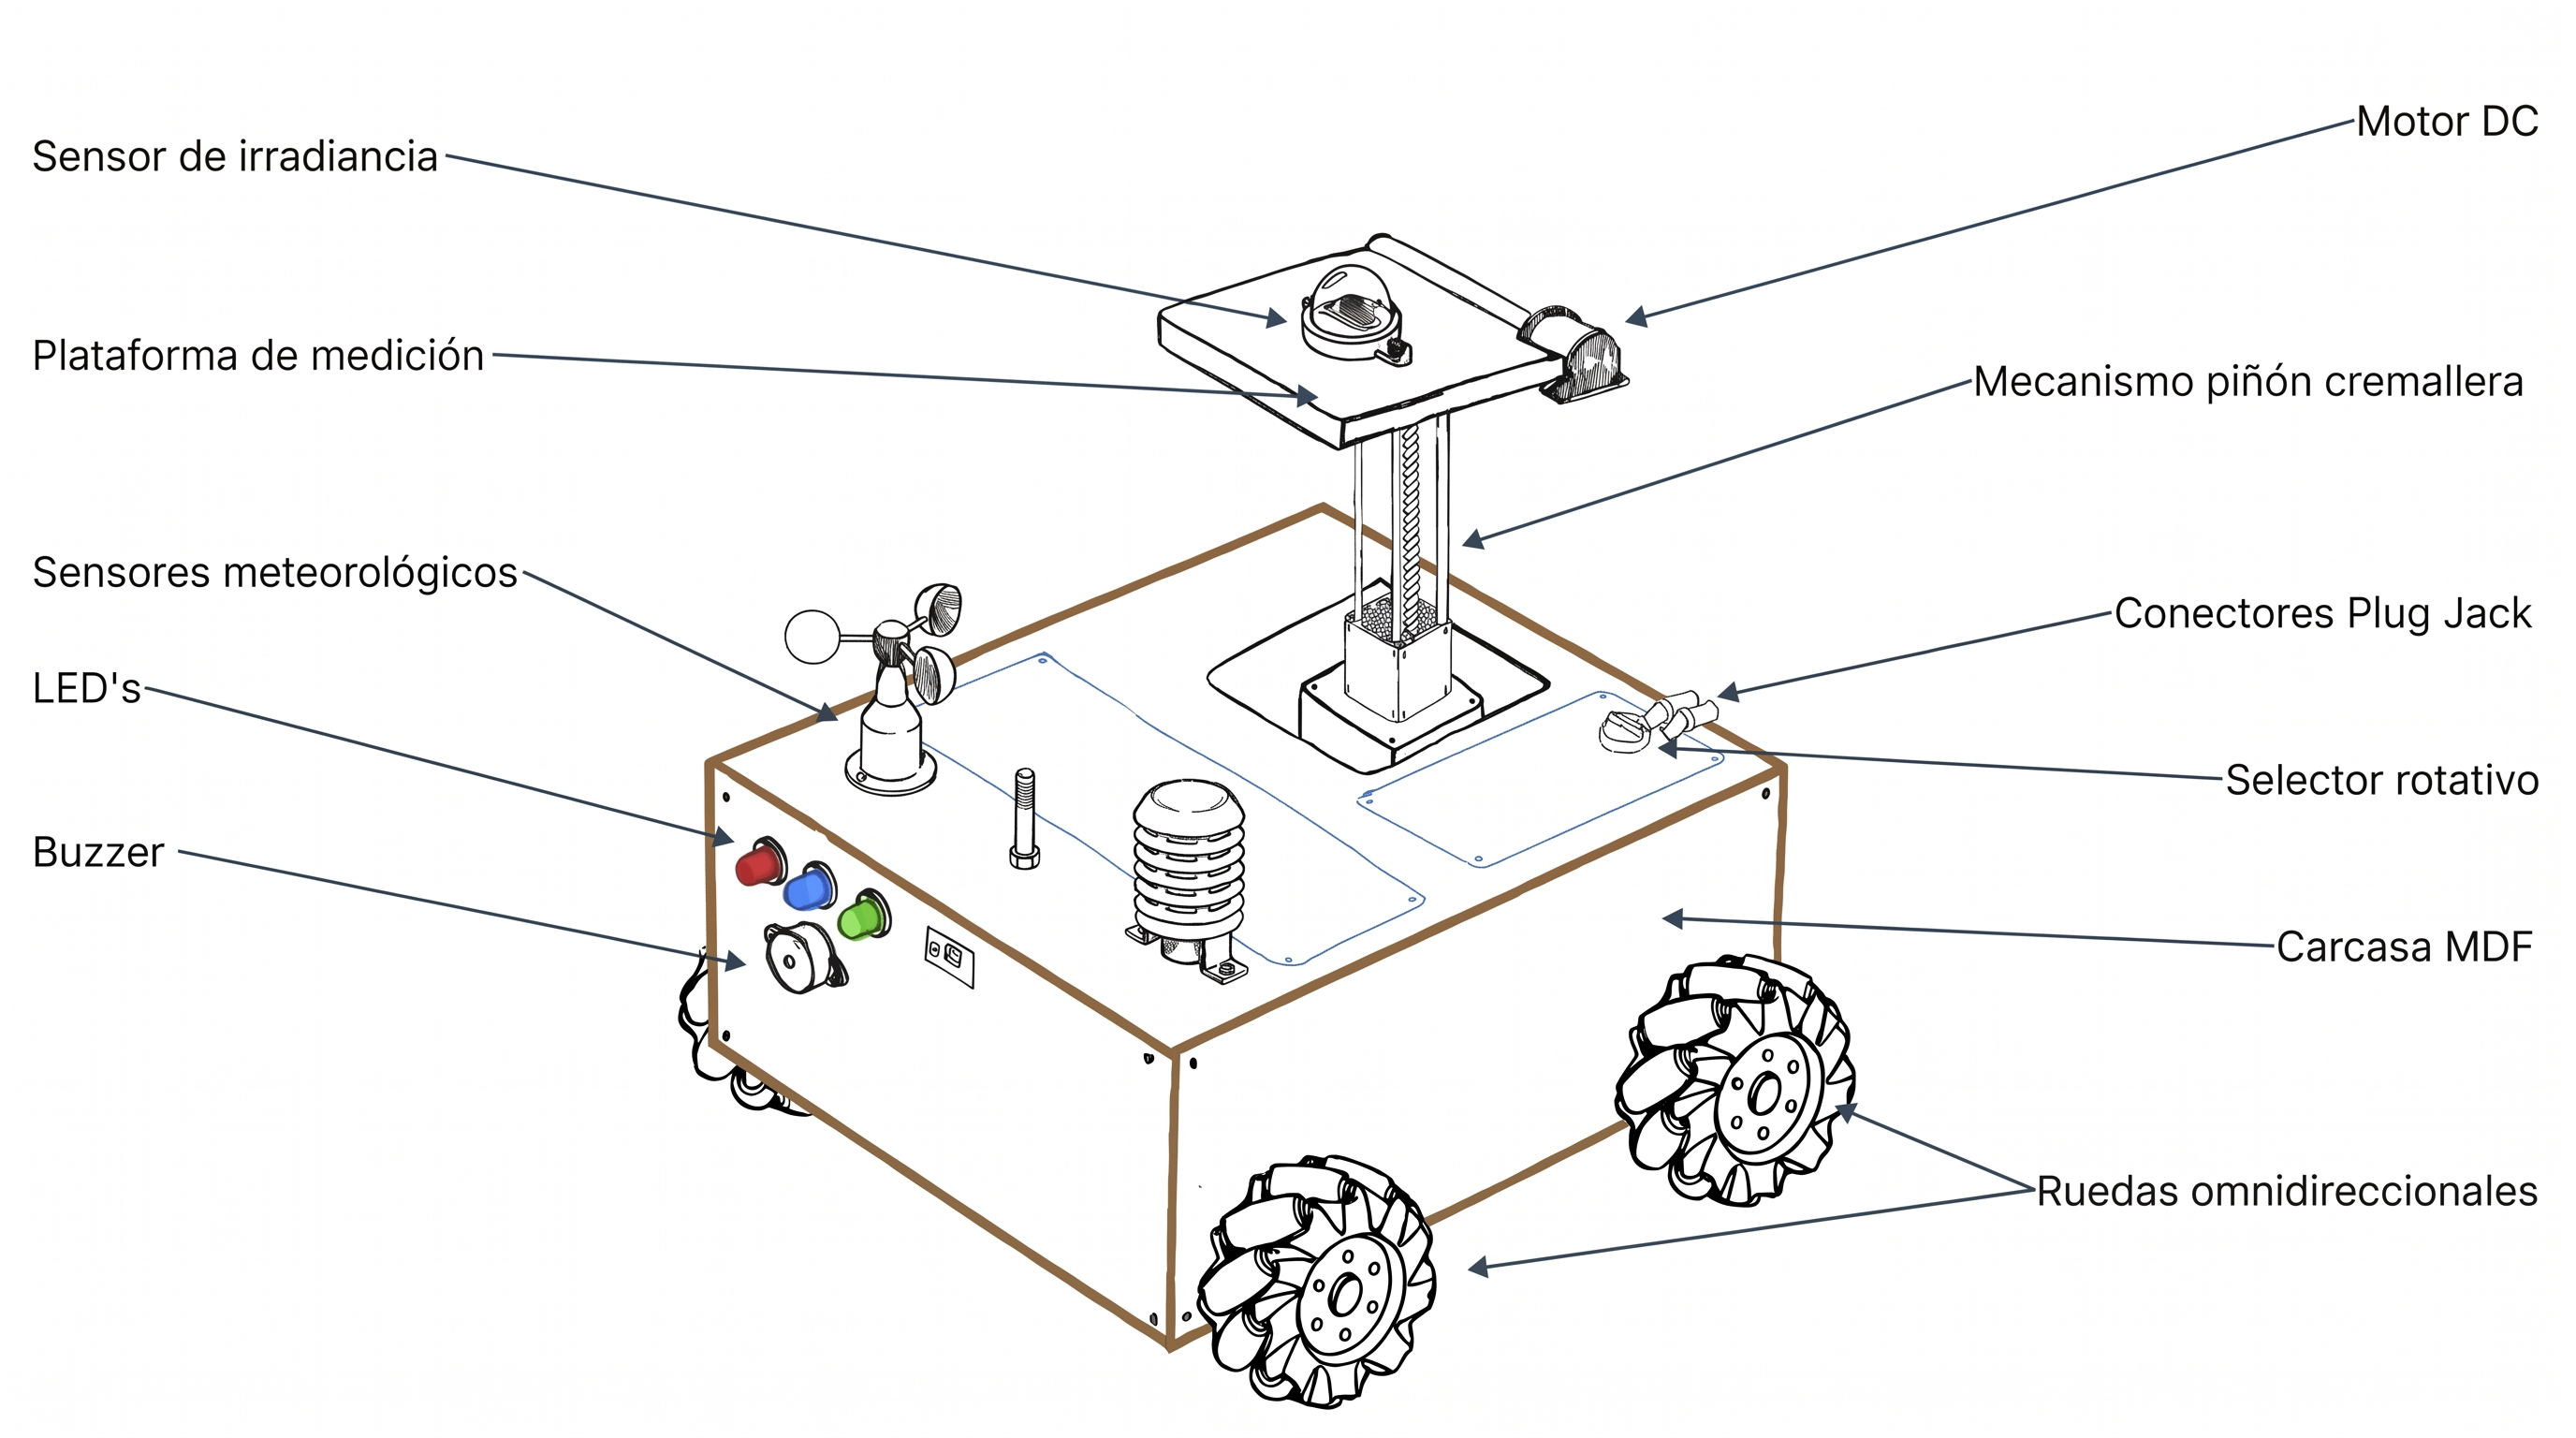
\includegraphics[width=\textwidth]{ImagenesConceptos/A-General.jpeg} \par\medskip
	
	\raggedright
	\footnotesize \textit{Nota.} Elaboración propia, asistida con IA generativa.
	\label{fig:AGeneral}
\end{figure}

\begin{figure}[H]
	% Fuerza la alineación izquierda y quita los ":" después del número
	\captionsetup{justification=raggedright, singlelinecheck=false, labelsep=none}
	
	\caption[Diseño interno de la solución 1.]{} 
	
	% Vspace negativo opcional para acercar el texto cursivo al número de figura
	\textit{Diseño interno de la solución 1.} \par\medskip
	
	\centering
	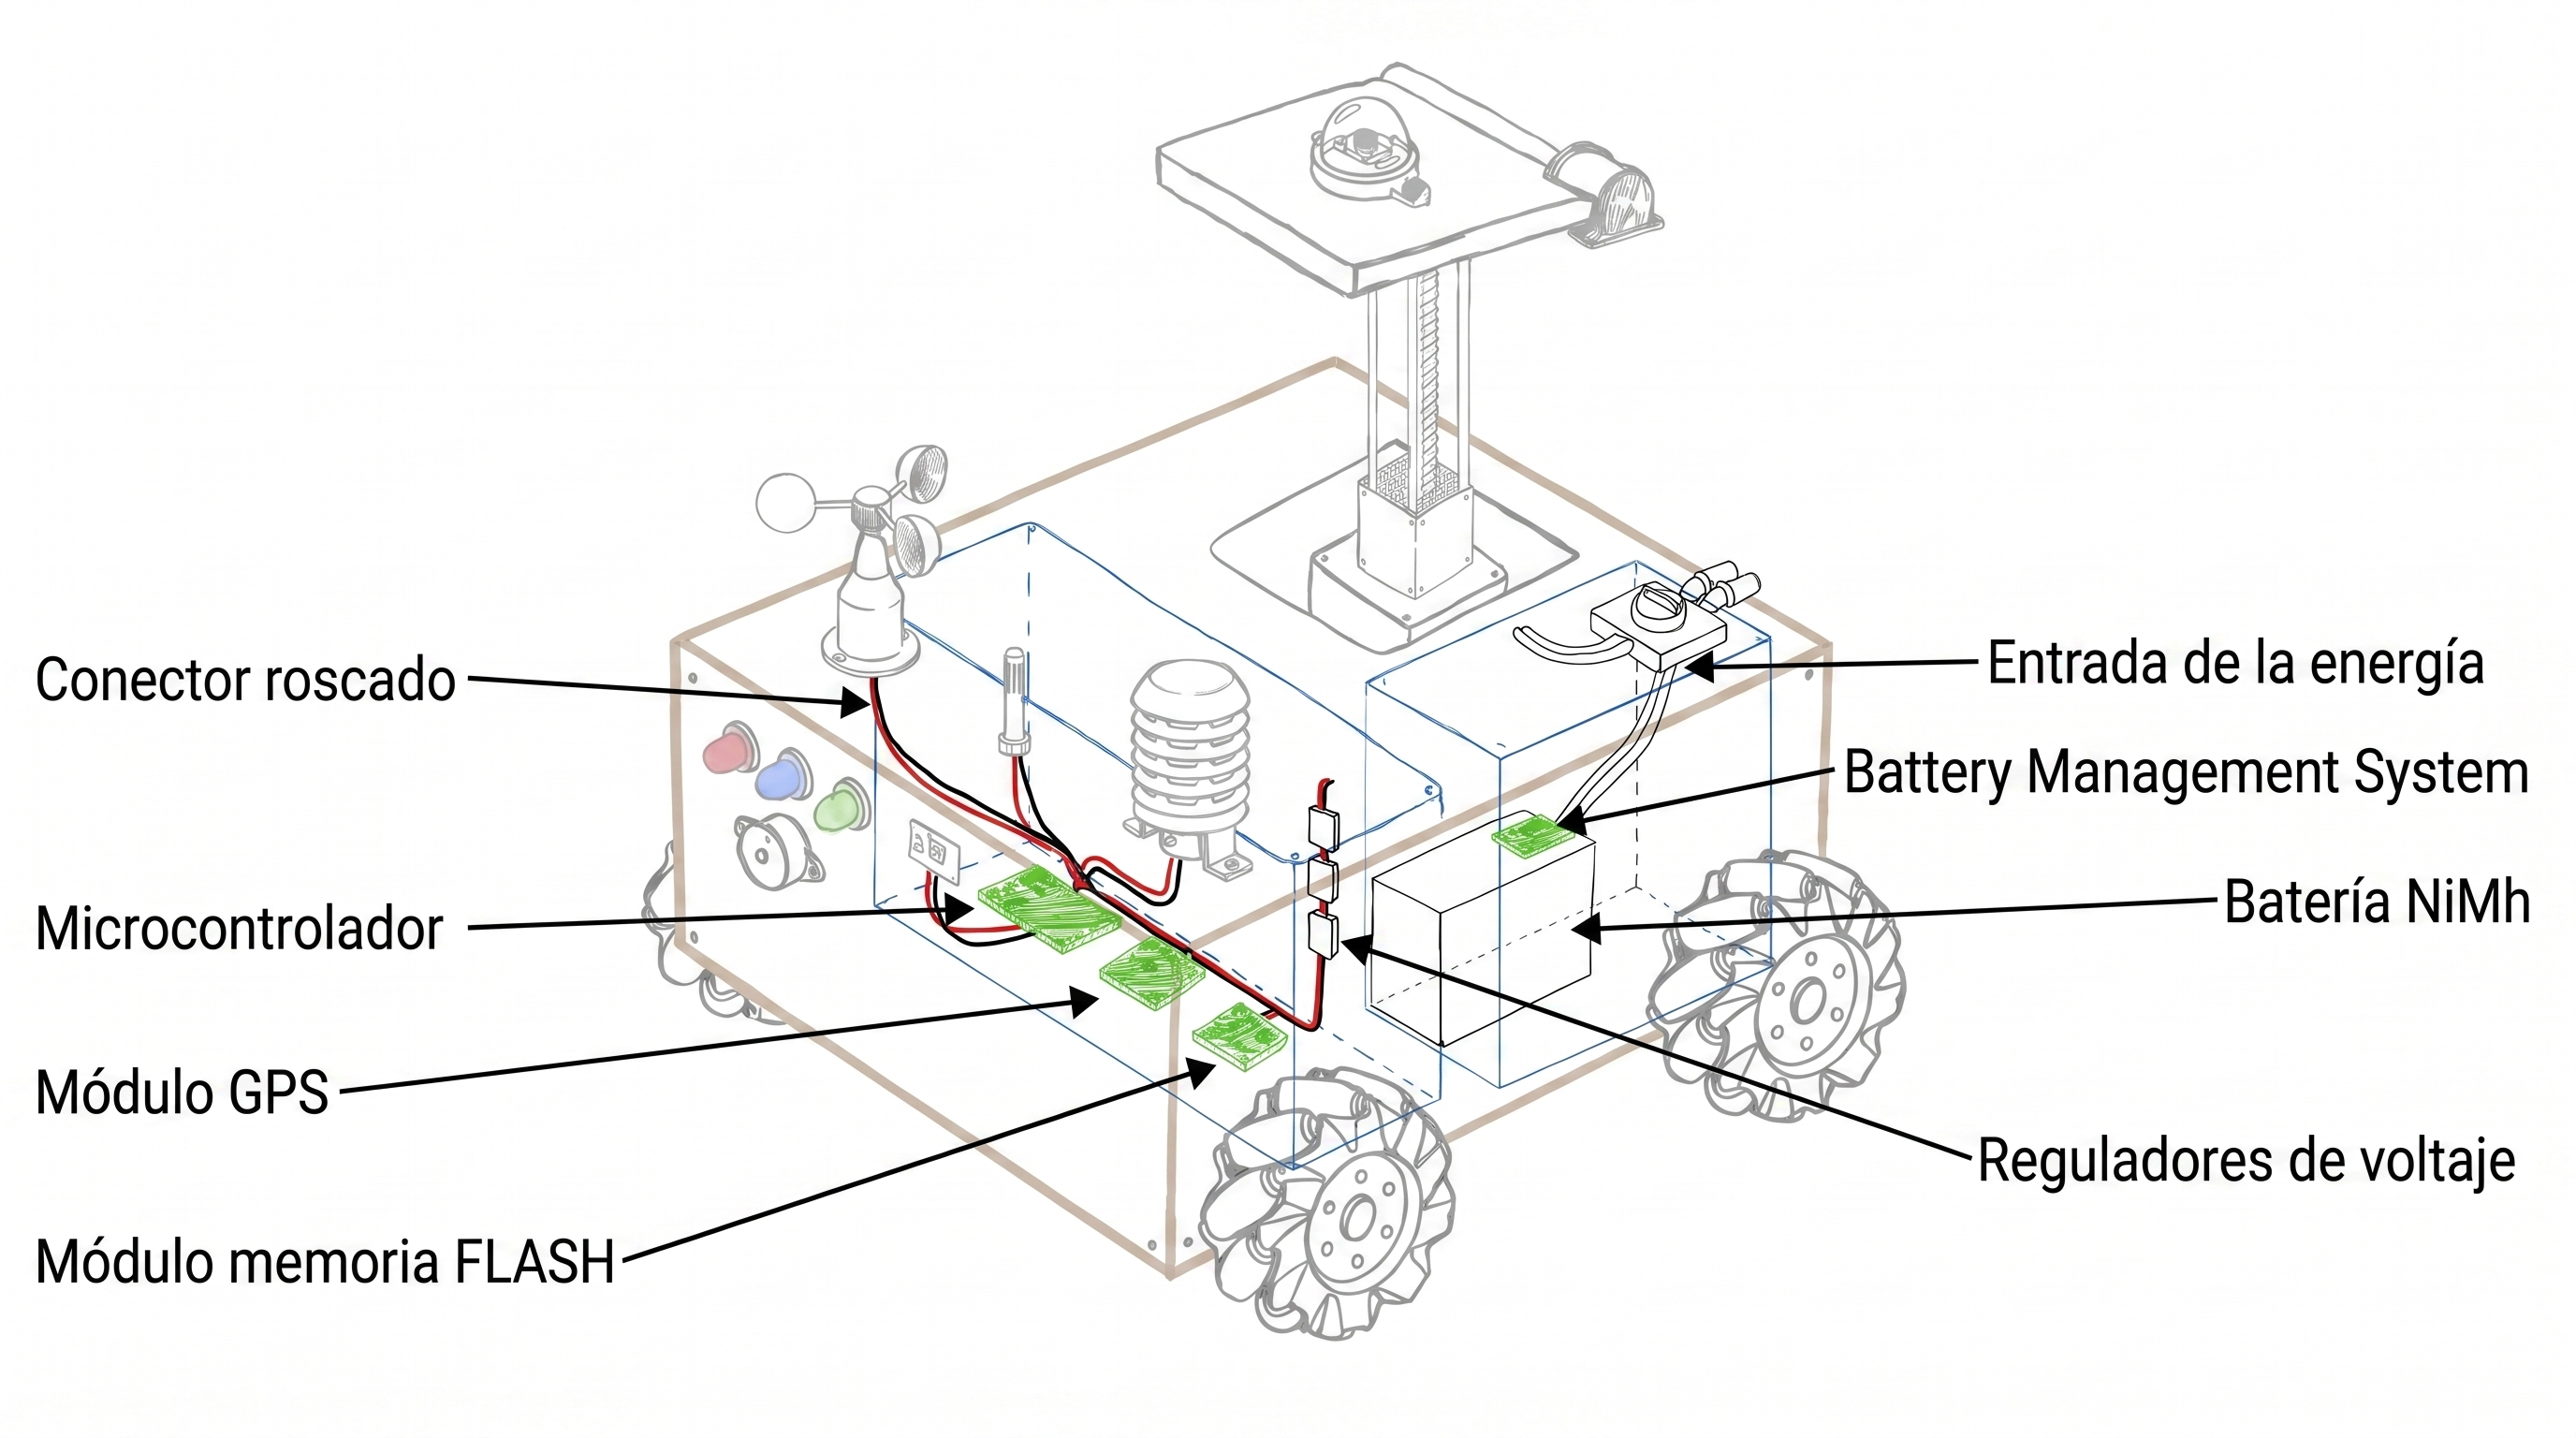
\includegraphics[width=\textwidth]{ImagenesConceptos/A-Interno.jpeg} \par\medskip
	
	\raggedright
	\footnotesize \textit{Nota.} Elaboración propia, asistida con IA generativa.
	\label{fig:AInterno}
\end{figure}

\section{Concepto de solución 2}

Este concepto representa un equilibrio óptimo entre robustez técnica, costo y capacidad de procesamiento para entornos de parques solares. A nivel mecánico y estructural, el equipo está construido sólidamente con una carcasa de aluminio y su desplazamiento se da por tracción diferencial mediante cuatro ruedas. Además, cuenta con una plataforma superior de instrumentación móvil que asegura gran precisión e inamovilidad gracias al uso de mecanismos de tornillo sin-fin y corona accionados por un servomotor DC. En cuanto a energía e interfaz, el robot presenta una alta confiabilidad operando con una batería de iones de litio protegida por sistemas de gestión de batería y reguladores de voltaje internos. Su interfaz exterior emplea borneras industriales para sus conexiones y cuenta con una pantalla LCD junto a una pantalla HMI lateral para interactuar e informar sobre su estado. Para la percepción y exploración, el sistema adquiere datos del entorno mediante sensores meteorológicos y un sensor de irradiancia ubicados en su plataforma elevadiza, emplea un módulo CMOS frontal para la visión por cámara, y transmite o recibe telemetría a través de una antena externa. Finalmente, en cuanto a control y lógica, el cerebro central del robot es una placa SBC que registra la información recopilada en un módulo de memoria microSD. Para ejecutar los cálculos complejos y procesar el video de la cámara, la SBC se apoya directamente en un Acelerador Edge IA, lo que le permite procesar el entorno de manera eficiente mientras utiliza control PID para los motores y traza su trayectoria con el Algoritmo Pure Pursuit.

\begin{figure}[H]
	% Fuerza la alineación izquierda y quita los ":" después del número
	\captionsetup{justification=raggedright, singlelinecheck=false, labelsep=none}
	
	\caption[Diseño general de la solución 2.]{} 
	
	% Vspace negativo opcional para acercar el texto cursivo al número de figura
	\textit{Diseño general de la solución 2.} \par\medskip
	
	\centering
	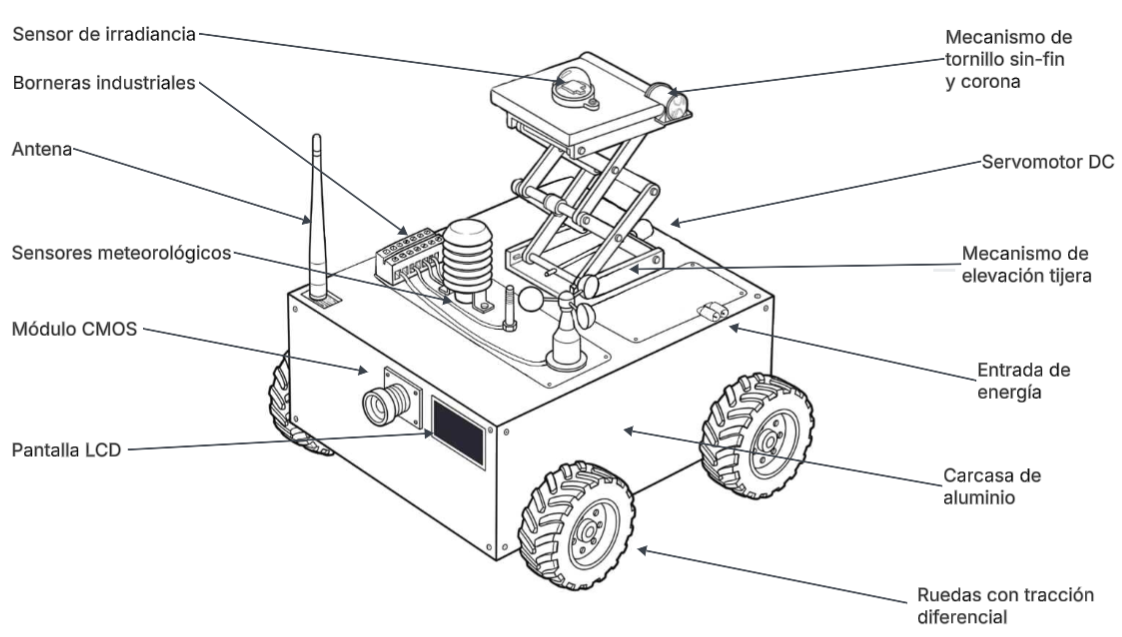
\includegraphics[width=\textwidth]{ImagenesConceptos/B-General.png} \par\medskip
	
	\raggedright
	\footnotesize \textit{Nota.} Elaboración propia, asistida con IA generativa.
	\label{fig:BGeneral}
\end{figure}

\begin{figure}[H]
	% Fuerza la alineación izquierda y quita los ":" después del número
	\captionsetup{justification=raggedright, singlelinecheck=false, labelsep=none}
	
	\caption[Diseño interno de la solución 2.]{} 
	
	% Vspace negativo opcional para acercar el texto cursivo al número de figura
	\textit{Diseño interno de la solución 2.} \par\medskip
	
	\centering
	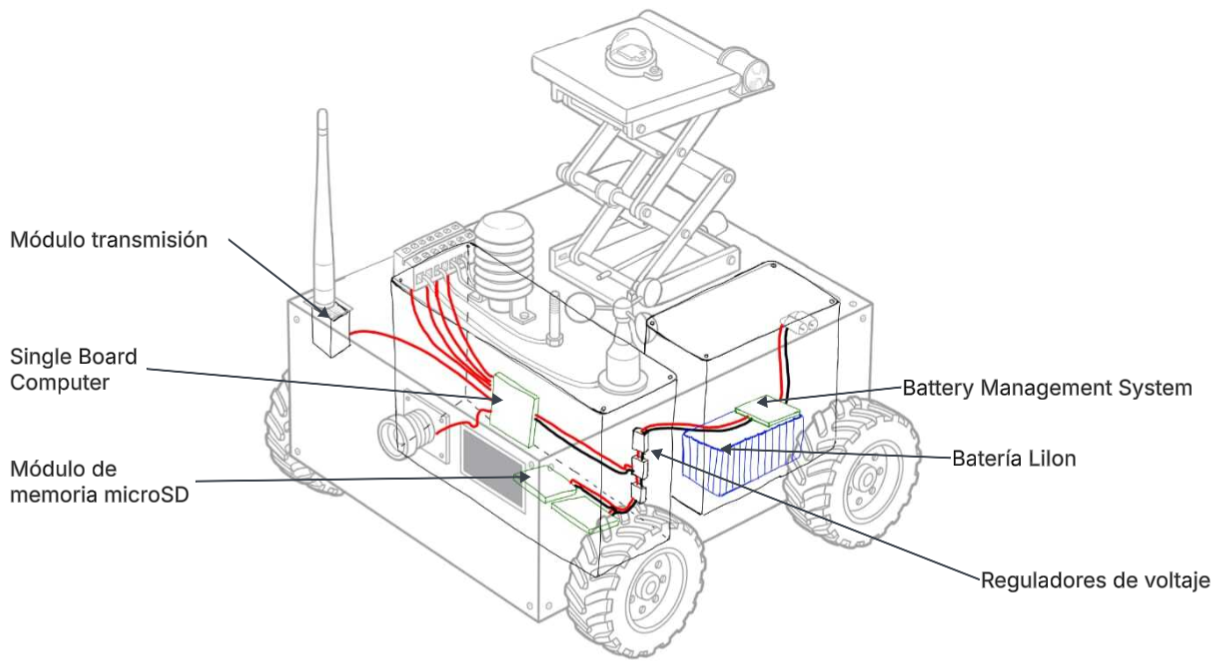
\includegraphics[width=\textwidth]{ImagenesConceptos/B-Interno.png} \par\medskip
	
	\raggedright
	\footnotesize \textit{Nota.} Elaboración propia, asistida con IA generativa.
	\label{fig:BInterno}
\end{figure}

\section{Concepto de solución 3}

El tercer concepto de soluciíon corresponde al nivel tecnológico industrial, diseñado para resistir las condiciones topográficas y climáticas más agresivas. Su estructura mecánica emplea un blindaje mediante una carcasa principal de acero y garantiza la movilidad en terrenos accidentados gracias a un sistema de ruedas con tracción de oruga que es impulsado internamente por un motorreductor DC. Además, el equipo integra una plataforma de medición que descansa sobre un actuador lineal vertical y opera mediante un motor DC acoplado a un mecanismo de correa dentada. En el apartado de energía e interfaz, el robot dispone de un sistema de carga exterior mediante contactos magnéticos, reguladores de voltaje internos y se alimenta con una batería LiPo protegida por un Battery Management System. Todo el cableado y la electrónica interna utilizan conexiones herméticas Deutsch, mientras que el chasis exterior se complementa con una pantalla HMI para la interacción directa y una sirena LED de señalización. La percepción y lectura del entorno están a cargo de un sensor LiDAR frontal, apoyado por sensores meteorológicos y un sensor de irradiancia montados en la plataforma superior. Finalmente, el control y la lógica del sistema son gobernados por un PLC, el cual trabaja en paralelo con un acelerador Edge IA para procesar eficientemente los datos del entorno, como la segmentación de nubes de puntos del LiDAR, permitiendo así una navegación avanzada.

\begin{figure}[H]
	% Fuerza la alineación izquierda y quita los ":" después del número
	\captionsetup{justification=raggedright, singlelinecheck=false, labelsep=none}
	
	\caption[Diseño general de la solución 3.]{} 
	
	% Vspace negativo opcional para acercar el texto cursivo al número de figura
	\textit{Diseño general de la solución 3.} \par\medskip
	
	\centering
	
\includegraphics[width=\textwidth]{ImagenesConceptos/C-General.png} \par\medskip
	
	\raggedright
	\footnotesize \textit{Nota.} Elaboración propia, asistida con IA generativa.
	\label{fig:CGeneral}
\end{figure}

\begin{figure}[H]
	% Fuerza la alineación izquierda y quita los ":" después del número
	\captionsetup{justification=raggedright, singlelinecheck=false, labelsep=none}
	
	\caption[Diseño interno de la solución 3.]{} 
	
	% Vspace negativo opcional para acercar el texto cursivo al número de figura
	\textit{Diseño interno de la solución 3.} \par\medskip
	
	\centering
	
\includegraphics[width=\textwidth]{ImagenesConceptos/C-Interno.png} \par\medskip
	
	\raggedright
	\footnotesize \textit{Nota.} Elaboración propia, asistida con IA generativa.
	\label{fig:CInterno}
\end{figure}

\section{Evaluación técnica}

\begin{table}[H]
	\captionsetup{justification=raggedright, singlelinecheck=false, labelsep=none}
	
	\caption[Matriz de Evaluación Técnica de Conceptos de Solución.]{} 
	\textit{Matriz de Evaluación Técnica de Conceptos de Solución.} \par\medskip
	
	\centering
	\footnotesize
	\renewcommand{\arraystretch}{1.3} 
	\begin{tabular}{|p{5.5cm}|c|c|c|c|c|c|c|c|c|}
		\hline
		\rowcolor[HTML]{D9E1F2} 
		\multirow{2}{*}{\textbf{Criterio de Evaluación}} & \multirow{2}{*}{\textbf{Peso (G)}} & \multicolumn{2}{c|}{\textbf{Solución 1}} & \multicolumn{2}{c|}{\textbf{Solución 2}} & \multicolumn{2}{c|}{\textbf{Solución 3}} & \multicolumn{2}{c|}{\textbf{Sol. Ideal}} \\ \cline{3-10}
		\rowcolor[HTML]{D9E1F2} 
		& & \textbf{P} & \textbf{GP} & \textbf{P} & \textbf{GP} & \textbf{P} & \textbf{GP} & \textbf{P} & \textbf{GP} \\ \hline
		\textbf{Geometría:}  (E) & 8 & 3 & 24 & 4 & 32 & 2 & 16 & 4 & 32 \\ \hline
		\textbf{Cinemática:}  (D) & 4 & 1 & 4 & 4 & 16 & 3 & 12 & 4 & 16 \\ \hline
		\textbf{Fuerzas:} (E) & 9 & 1 & 9 & 3 & 27 & 4 & 36 & 4 & 36 \\ \hline
		\textbf{Energía:} (E) & 9 & 2 & 18 & 4 & 36 & 2 & 18 & 4 & 36 \\ \hline
		\textbf{Materia:} (E) & 8 & 1 & 8 & 3 & 24 & 4 & 32 & 4 & 32 \\ \hline
		\textbf{Materia (Térmica):} (E) & 7 & 1 & 7 & 4 & 28 & 3 & 21 & 4 & 28 \\ \hline
		\textbf{Señales:} (E) & 10 & 2 & 20 & 3 & 30 & 4 & 40 & 4 & 40 \\ \hline
		\textbf{Control:} (E) & 9 & 2 & 18 & 3 & 27 & 4 & 36 & 4 & 36 \\ \hline
		\textbf{Comunicación:} (E) & 8 & 2 & 16 & 4 & 32 & 3 & 24 & 4 & 32 \\ \hline
		\textbf{Mantenimiento:}  (D) & 6 & 2 & 12 & 2 & 12 & 4 & 24 & 4 & 24 \\ \hline
		\textbf{Seguridad:}  (D) & 5 & 1 & 5 & 2 & 10 & 4 & 20 & 4 & 20 \\ \hline\hline
		
		\multicolumn{2}{|r|}{\textbf{Puntaje Total ($Pt$)}} & \multicolumn{2}{c|}{\textbf{141}} & \multicolumn{2}{c|}{\textbf{274}} & \multicolumn{2}{c|}{\textbf{279}} & \multicolumn{2}{c|}{\textbf{332}} \\ \hline
		\multicolumn{2}{|r|}{\textbf{Valor Técnico ($X_i$)}} & \multicolumn{2}{c|}{\textbf{0.42}} & \multicolumn{2}{c|}{\textbf{0.83}} & \multicolumn{2}{c|}{\textbf{0.84}} & \multicolumn{2}{c|}{\textbf{1.00}} \\ \hline
	\end{tabular} \par\medskip
	
	\raggedright
	\scriptsize \textit{Nota.} Elaboración propia. G = Peso del requerimiento; P = Puntaje (escala del 0 al 4); GP = Puntaje Ponderado ($P \times G$); E = Exigencia; D = Deseo. El Valor Técnico ($X_i$) se calcula dividiendo el Puntaje Total de la solución entre el Puntaje Total de la Solución Ideal ($Pt / 332$).
	\label{tab:matriz_evaluacion_tecnica}
\end{table}

\begin{enumerate}
	\item \textbf{Geometría:} Para evaluar la volumetría y masa del equipo, la solución 2 destaca con un puntaje igual a 4, ya que su chasis de aluminio V-Slot garantiza un diseño compacto y ligero debido a su baja densidad y resistencia decente \citep{}, también cumple con las normativas ergonómicas para el manejo de cargas de los operarios \citep{Figgis2025}. Por otro lado, la solución 1 cuenta con un puntaje igual a 3, pues a pesar de ser ligera por utilizar piezas impresas en 3D y MDF, requiere de mayores espesores para mantener su rigidez, acercándose peligrosamente al límite volumétrico permitido. Por último, a la solución 3 se le asigna un puntaje igual a 2, debido a que corre el riesgo de incumplir la restricción ergonómica al exceder los 20 kg de peso por culpa de su carcasa de acero y su sistema de tracción por orugas.
	
	\item \textbf{Cinemática:} Respecto al desplazamiento dinámico en el terreno, la solución 2 es la más destacada con un puntaje igual a 4, pues al emplear la tracción diferencial de 4 ruedas ofrece la máxima velocidad y eficiencia para alcanzar con holgura el objetivo de 1 m/s \citep{Figgis2025}. Le sigue la solución 3, con un puntaje igual a 3, que cumple con el requerimiento pero sacrifica parte de su agilidad y velocidad nominal debido a la alta fricción mecánica que generan sus orugas contra el suelo \citep{}. En contraste, la solución 1 obtiene un puntaje igual a 1, dado que sus ruedas omnidireccionales resultan ser difícilmente operables y lentas sobre la topografía de una planta solar \citep{}.
	
	\item \textbf{Fuerzas:} En la evaluación de la tracción, orientada a superar pendientes irregulares de hasta $14^\circ$, la solución 3 se posiciona como la alternativa más apta con un puntaje igual a 4, utilizando un tren de orugas que distribuye el peso de manera uniforme para evitar deslizamientos o volcaduras en los terrenos \citep{}. A continuación, la solución 2 recibe un puntaje igual a 3, ya que su tracción a 4 ruedas es mecánicamente robusta, pero presenta cierto riesgo de patinar si transita sobre tramos con arena suelta y alta inclinación. Finalmente, la solución 1 se queda con un puntaje igual a 1, porque su diseño ligero carece del torque y el agarre necesarios para escalar pendientes pronunciadas \citep{}.
	
	\item \textbf{Energía:} Respecto a la exigencia de proveer al menos una hora de autonomía, la solución 2 logra el mejor desempeño con un puntaje igual a 4, gracias a la altísima densidad energética de sus baterías Li-Ion combinadas con un chasis que demanda poca potencia motriz \citep{}. La solución 3 se sitúa al límite del requerimiento con un puntaje igual a 2, puesto que, aunque utiliza baterías LiPO de alta descarga, el excesivo peso del acero estructural y la fricción constante de sus orugas penalizan drásticamente su consumo de energía \citep{}. La solución 1 recibe un puntaje igual a 2, siendo ineficiente al depender de baterías NiMH pesadas que tienen dificultades para sostener la operación ininterrumpida de los motores.
	
	\item \textbf{Materia:} Frente a la protección contra impactos mecánicos y la intemperie, la solución 3 lidera con un puntaje igual a 4, ofreciendo la máxima protección industrial al estar completamente encapsulada en acero inoxidable y chapas de acero estructural. En un nivel intermedio se encuentra la solución 2, con un puntaje igual a 3, cuya caja de chapa de aluminio brinda una excelente hermeticidad frente a la corrosión, aunque puede deformarse con mayor facilidad ante golpes directos. La solución 1 resulta inaceptable con un puntaje igual a 1, ya que ofrece la menor resistencia a impacto del exterior con un chasis de MDF y carcasa plástica.
	
	\item \textbf{Materia (Térmica):} Para garantizar la operación continua sin sobrecalentamientos de acuerdo con los requerimientos operativos de la instrumentación \citep{}, la solución 2 resulta óptima con un puntaje igual a 4, ya que su caja de chapa de aluminio actúa como un excelente disipador térmico que protege eficientemente la electrónica interna. La solución 3 recibe un puntaje aceptable igual a 3, se penaliza ligeramente porque su carcasa de acero tiende a retener mucho más calor bajo el sol \citep{}, lo que podría generar fallas térmicas en sus componentes internos. Por el contrario, a la solución 1 se le asigna un puntaje igual a 1, fallando en este aspecto debido a que carece de una correcta disipación térmica y sus polímeros 3D podrían deformarse ante la exposición continua.
	
	\item \textbf{Señales:} En cuanto a la precisión exigida por las normas internacionales, la solución 3 es netamente superior con un puntaje igual a 4, logrando integrar sensores industriales de gran exactitud y robustez\citep{}. La solución 2 obtiene un buen puntaje igual a 3, ya que posee una precisión general destacable, pero depende de un módulo CMOS visual que es vulnerable a los reflejos de los paneles solares. La solución 1 demuestra ser menos eficiente, recibiendo un puntaje igual a 2 al emplear sensores básicos y mecánicos que son propensos a sufrir derivas en los datos.
	
	\item \textbf{Control:} Para evaluar la capacidad de evadir obstáculos y recalcular rutas inmediatamente, la solución 3 domina con un puntaje igual a 4, apoyándose en un avanzado acelerador Edge IA y un LiDAR 3D que procesan nubes de puntos espaciales en tiempo real \citep{}. La solución 2, con un puntaje igual a 3, cuenta con una placa SBC de buen rendimiento, pero el algoritmo de flujo óptico de la cámara pierde gran parte de su efectividad si el entorno está muy polvoriento o la iluminación varía. A la solución 1 se le otorga un puntaje igual a 2 al ser la más limitada computacionalmente, dado que su microcontrolador podrá generar falsos positivos al basarse en comparación de umbrales.
	
	\item \textbf{Comunicación:} Al evaluar la estabilidad y transmisión de telemetría, la solución 2 es la alternativa más atractiva con un puntaje igual a 4, al incorporar un módulo LoRa que es excelente para alcanzar grandes distancias en parques extensos consumiendo un mínimo de electricidad \citep{}. La solución 3 recibe un puntaje igual a 3, pues a pesar de que emplea una conexión celular LTE-M con mayor ancho de banda, depende enteramente de la cobertura de red local, lo cual requiere de infraestructura adicional. Por su parte, a la solución 1 se le asigna un puntaje igual a 2, resultando inviable porque su red Wi-Fi requiere de múltiples nodos para mantener cobertura a lo largo de la planta \citep{}.
	
	\item \textbf{Mantenimiento:} Con el propósito de lidiar con la acumulación de suciedad en el entorno, la solución 3 resulta ser la más resiliente con un puntaje igual a 4, ya que los radares y contactos magnéticos logran operar incluso estando cubiertos de polvo \citep{}. La solución 2 obtiene un puntaje igual a 2, puesto que requerirá de mantenimientos manuales mucho más recurrentes, debido a que la acumulación de arena en el lente de la cámara afectará directamente la visión del robot. Finalmente, la solución 1 cuenta con un puntaje igual a 2, utilizando potenciómetros y fines de carrera con piezas móviles que se podrían dañar con la tierra.
	
	\item \textbf{Seguridad:} Frente a eventuales incidentes en planta, la solución 3 garantiza la mayor protección preventiva con un puntaje igual a 4, al estar dotada de disyuntores termomagnéticos y poseer un diseño pesado difícil de volcar \citep{}. La solución 2, con un puntaje igual a 3, logra reaccionar casi instantáneamente ante cortocircuitos gracias a sus protectores eFuse, pero su ligereza la hace levemente propensa a perder estabilidad en baches profundos. Para concluir, a la solución 1 se le asigna un puntaje igual a 1 al considerarse muy insegura en exteriores, dependiendo de fusibles cerámicos básicos y de una estructura liviana demasiado frágil ante vientos fuertes.
\end{enumerate}

\section{Evaluación económica}

\begin{table}[H]
	\captionsetup{justification=raggedright, singlelinecheck=false, labelsep=none}
	
	\caption[Matriz de Evaluación Económica de Conceptos de Solución.]{} 
	\textit{Matriz de Evaluación Económica de Conceptos de Solución.} \par\medskip
	
	\centering
	\footnotesize
	\renewcommand{\arraystretch}{1.8} 
	\begin{tabular}{|c|p{4.5cm}|c|c|c|c|c|c|c|c|c|}
		\hline
		\rowcolor[HTML]{D9D9D9} 
		\multicolumn{3}{|c|}{\textbf{Variantes de Concepto/Proyecto}} & \multicolumn{2}{c|}{\textbf{Solución 1}} & \multicolumn{2}{c|}{\textbf{Solución 2}} & \multicolumn{2}{c|}{\textbf{Solución 3}} & \multicolumn{2}{c|}{\textbf{Sol. Ideal}} \\ \hline
		\rowcolor[HTML]{D9D9D9} 
		\textbf{N$^{\circ}$} & \multicolumn{1}{c|}{\textbf{Criterio de Evaluación}} & \textbf{G} & \textbf{P} & \textbf{GP} & \textbf{P} & \textbf{GP} & \textbf{P} & \textbf{GP} & \textbf{P} & \textbf{GP} \\ \hline
		
		1 & Costo de Tecnología & 4 & 3 & 12 & 3 & 12 & 2 & 8 & 4 & 16 \\ \hline
		2 & Costo de Mantenimiento & 3 & 4 & 12 & 2 & 6 & 2 & 6 & 4 & 12 \\ \hline
		3 & Disponibilidad de Materiales & 4 & 4 & 16 & 3 & 12 & 1 & 4 & 4 & 16 \\ \hline
		4 & Costo de Fabricación & 3 & 3 & 9 & 2 & 6 & 1 & 3 & 4 & 12 \\ \hline
		
		\multicolumn{2}{|r|}{\textbf{Puntaje Total}} & \textbf{14} & \multicolumn{2}{c|}{\textbf{49}} & \multicolumn{2}{c|}{\textbf{36}} & \multicolumn{2}{c|}{\textbf{21}} & \multicolumn{2}{c|}{\textbf{56}} \\ \hline
		\multicolumn{3}{|r|}{\textbf{Valor Económico ($Y_i$)}} & \multicolumn{2}{c|}{\textbf{0.88}} & \multicolumn{2}{c|}{\textbf{0.64}} & \multicolumn{2}{c|}{\textbf{0.38}} & \multicolumn{2}{c|}{\textbf{1.00}} \\ \hline

	\end{tabular} \par\medskip
	
	\raggedright
	\scriptsize \textit{Nota.} Elaboración propia. G = Peso del requerimiento; P = Puntaje (escala del 0 al 4); GP = Puntaje Ponderado ($P \times G$). El Valor Económico ($Y_i$) se calcula dividiendo el Puntaje Total de cada alternativa entre el total de la Solución Ideal ($56$).
	\label{tab:matriz_evaluacion_economica}
\end{table}

\begin{enumerate}
	\item \textbf{Costo de Tecnología:} En cuanto a la inversión necesaria para adquirir los componentes, la solución 1 y la solución 2 obtienen un buen puntaje igual a 3, dado que basan su arquitectura en componentes accesibles y módulos electrónicos de costo estandarizado. Por el contrario, a la solución 3 se le asigna un puntaje igual a 2, puesto que la integración de componentes de grado altamente industrial, como un la PLC, incrementa de manera drástica el costo de capital inicial del sistema, reduciendo su viabilidad para una producción en serie.
	
	\item \textbf{Costo de Mantenimiento:} Para evaluar los gastos operativos a largo plazo, la solución 1 destaca con el mejor puntaje igual a 4, debido a que el reemplazo de sus piezas y sensores básicos resulta económico frente a posibles daños por la intemperie. Tanto la solución 2 como la solución 3 reciben un puntaje igual a 2, ya que implican mayores gastos operativos continuos; la solución 2 exigirá rutinas de limpieza frecuentes para la lente de su cámara CMOS, mientras que la solución 3 demandará un mantenimiento mecánico mucho más costoso para la lubricación de sus ruedas de tracción de oruga y la calibración de la instrumentación industrial.
	
	\item \textbf{Disponibilidad de Materiales:} En cuanto a la facilidad para adquirir los repuestos en el mercado, la solución 1 obtiene un puntaje igual a 4, puesto que aprovecha la amplia disponibilidad local de polímeros genéricos, láminas de MDF y ecosistemas electrónicos de hardware libre, evitando procesos de importación \citep{}. Por su parte, la solución 2 obtiene un puntaje de 3, ya que cuenta con tecnologías más especializadas que no siempre cuentan con un stock local. De forma similar, la solución 3 tiene un puntaje de 1, dado que cuenta con componentes de grado industrial que están sujetas a demoras por la cadena de suministro internacional y requieren procesos complejos de importación \citep{}.
	
	\item \textbf{Costo de Fabricación:} Finalmente, respecto a la manufactura y ensamblaje, la solución 1 lidera con un puntaje igual a 3, ya que la fabricación basada en corte láser e impresión 3D permite producir piezas únicas con un costo muy bajo, eliminando por completo la necesidad de invertir en herramientas de conformado especializadas \citep{}. La solución 2 recibe un puntaje de 2; aunque utilice perfiles modulares V-Slot que facilitan el ensamblaje, requiere de procesos de mecanizado para su caja de aluminio, mientras que la solución 3 recibe un puntaje de 1, pues exige una inversión considerable  para los procesos de soldadura y conformado de acero, así como de sus sensores y controladores industriales.
\end{enumerate}

\section{Concepto de solución óptimo}

Tras someter las alternativas de diseño a la evaluación técnica y económica, se declara a la solución 2 como el concepto de solución óptimo (ver Figura \ref{fig:EvalTecEc}). Al proyectar los puntajes en el gráfico de evaluación técnico-económica, esta alternativa presenta el mejor nivel de convergencia hacia la diagonal ideal, ofreciendo un excelenete desempeño industrial técnico sin incurrir en los costos excesivos.

\begin{figure}[H]

	\captionsetup{justification=raggedright, singlelinecheck=false, labelsep=none}
	
	\caption[Elaboración técnica económica de las tres soluciones propuestas.]{} 
	
	\textit{Elaboración técnica económica de las tres soluciones propuestas.} \par\medskip
	
	\centering
	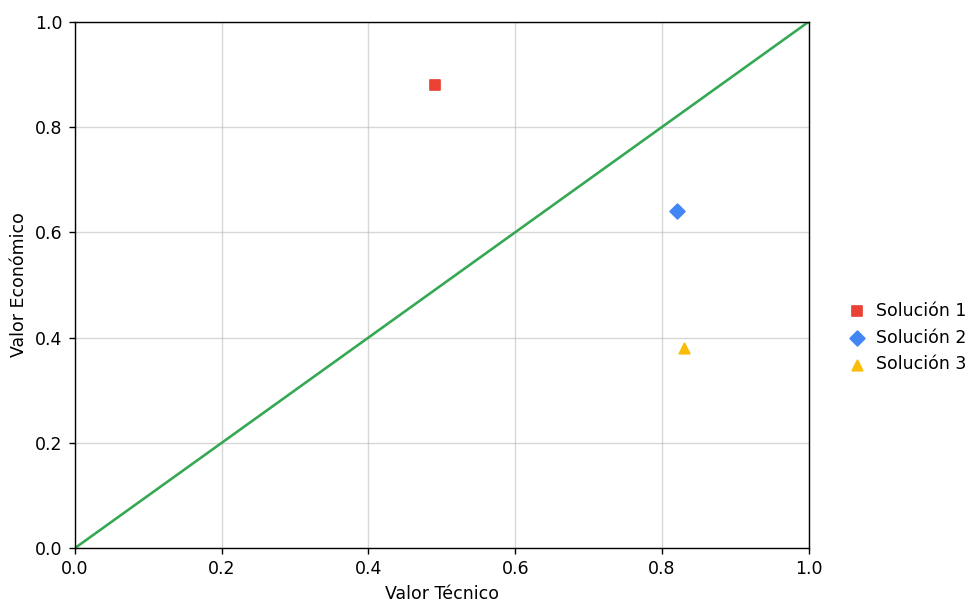
\includegraphics[width=\textwidth]{Imagenes/evtecec.png} \par\medskip
	
	\raggedright
	\footnotesize \textit{Nota.} Elaboración propia.
	\label{fig:EvalTecEc}
\end{figure}


\subsection{Arquitectura de control del concepto óptimo}

\subsubsection{Diagrama de flujo general} 

En la Figura \ref{fig:DiagramaFlujoGeneral}, se detalla la secuencia lógica de arranque y la arquitectura multitarea que gobierna la computadora principal del robot. El proceso inicia con la energización del hardware, donde el sistema operativo inicializa los buses de comunicación y declara una variable global de estado o Flag de Alerta en valor nulo. Posteriormente, el equipo entra en un estado de espera hasta recibir el comando inalámbrico de inicio por parte del operario.

Una vez activado, el software ejecuta una bifurcación propia de arquitecturas orientadas a eventos, dividiendo el procesamiento en hilos paralelos que operan de forma concurrente: un hilo de navegación, un hilo de telemetría y un hilo supervisor de seguridad. En lugar de que cada subproceso gestione sus propias condiciones de parada, los hilos paralelos operan exclusivamente como publicadores de estado. Simultáneamente, el hilo supervisor evalúa la Flag de Alerta de forma continua; si detecta un cambio de estado a valor activo, el supervisor ejecuta una interrupción de máxima prioridad que anula la tracción y transita al sistema hacia un modo seguro.

\begin{figure}[H]
	\captionsetup{justification=raggedright, singlelinecheck=false, labelsep=none}
	
	\caption[Diagrama de flujo de proceso general.]{} 
	
	\textit{Diagrama de flujo de proceso general.} \par\medskip
	
	\centering
	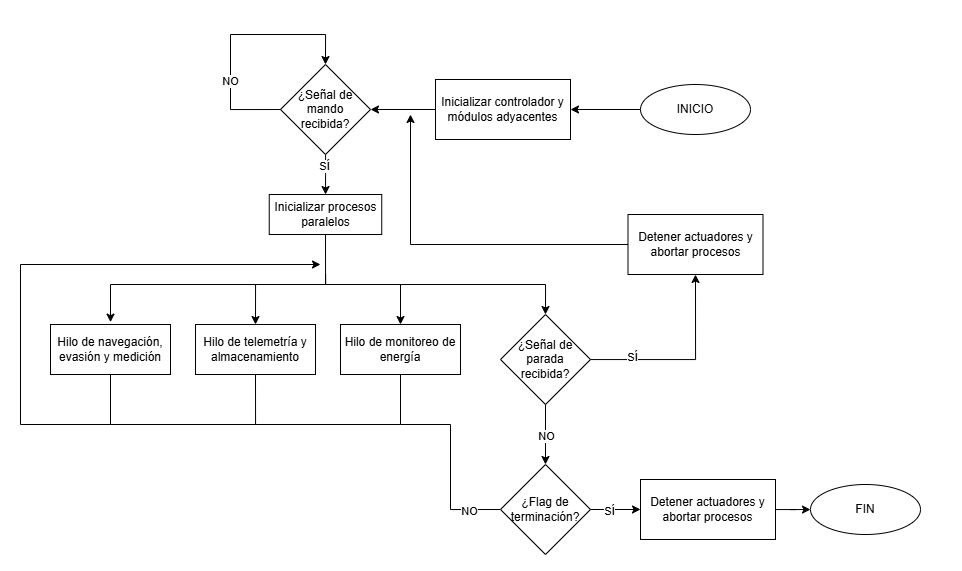
\includegraphics[width=\textwidth]{Imagenes/DiagramaFlujoGeneralTFC1_v2.png} \par\medskip
	
	\raggedright
	\footnotesize \textit{Nota.} Elaboración propia.
	\label{fig:DiagramaFlujoGeneral}
\end{figure}

\subsubsection{Lazo de control del movimiento del robot}

El desplazamiento autónomo del vehículo se rige mediante un lazo de control cerrado en cascada que integra el seguimiento espacial y la regulación de velocidad. Como se observa en la Figura \ref{fig:LazoControl}, la referencia del sistema se calcula dinámicamente comparando la ruta predefinida con las coordenadas espaciales retroalimentadas por la antena GPS de parche cerámico y la orientación provista por la unidad IMU. Esta fusión de datos alimenta al algoritmo geométrico Pure Pursuit, el cual calcula el error de desvío lateral para definir el ángulo de corrección requerido.

De forma paralela, la retroalimentación de los encoders rotativos determina el error respecto a la velocidad nominal operativa de 1 m/s. El controlador central, mediante un algoritmo PID, amalgama ambos errores para generar y distribuir las señales de Modulación por Ancho de Pulsos hacia los actuadores. Al tratarse de un chasis de tracción diferencial, el PID varía la potencia entre los flancos izquierdo y derecho para corregir el rumbo y mantener al robot sobre la trayectoria ideal sin interrumpir su avance.

\begin{figure}[H]
	\captionsetup{justification=raggedright, singlelinecheck=false, labelsep=none}
	
	\caption[Lazo de control del movimiento de traslación del robot.]{} 
	
	\textit{Lazo de control del movimiento de traslación del robot.} \par\medskip
	
	\centering
	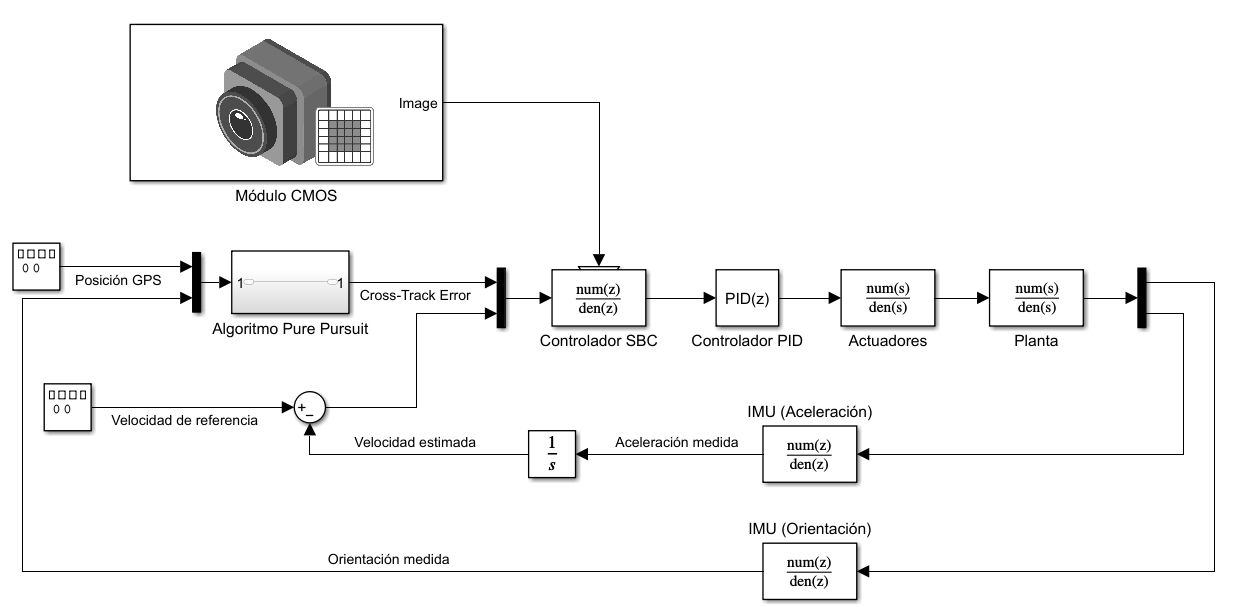
\includegraphics[width=\textwidth]{Imagenes/LazoControlSolucionOptima.png} \par\medskip
	
	\raggedright
	\footnotesize \textit{Nota.} Elaboración propia.
	\label{fig:LazoControl}
\end{figure}

\subsubsection{Topología de red}

La arquitectura de comunicaciones, vista en la Figura \ref{fig:TopologiaRed}, del sistema emplea una topología punto a punto fundamentada en el protocolo de radiofrecuencia LoRa. En este esquema, el robot de inspección actúa como un nodo terminal móvil equipado con un módulo transceptor LoRa que concentra los datos meteorológicos procesados.

La capa de red establece un enlace bidireccional de baja potencia y largo alcance con la estación base o Gateway ubicada en las instalaciones del parque fotovoltaico, garantizando una cobertura efectiva superior a los 200 metros. El enlace de subida se encarga de transmitir los paquetes de telemetría y alertas de obstáculos hacia el servidor central para su visualización y almacenamiento, mientras que el enlace de bajada permite que el dispositivo escuche continuamente comandos del exterior, posibilitando la recepción de instrucciones críticas como el telecomando de parada remota emitido por el operario.

\begin{figure}[H]
	\captionsetup{justification=raggedright, singlelinecheck=false, labelsep=none}
	
	\caption[Topología de red con los robots como nodos.]{} 
	
	\textit{Topología de red con los robots como nodos.} \par\medskip
	
	\centering
	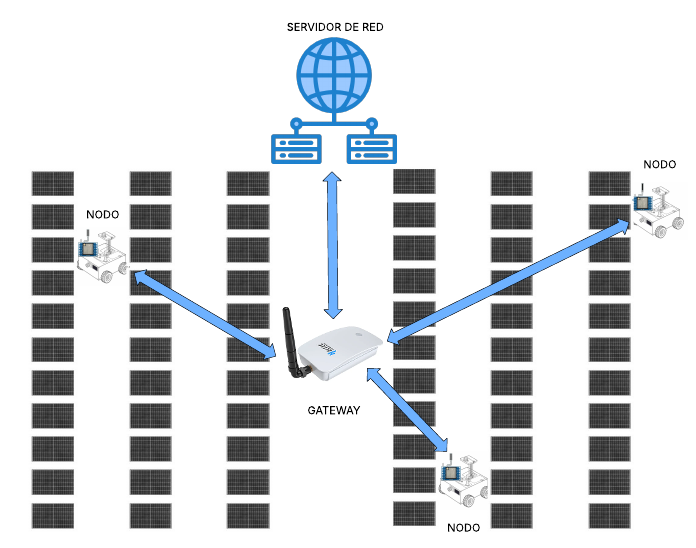
\includegraphics[width=\textwidth]{Imagenes/TopologiaRedTFC1.png} \par\medskip
	
	\raggedright
	\footnotesize \textit{Nota.} Elaboración propia.
	\label{fig:TopologiaRed}
\end{figure}


%%%%
\subsection{Arquitectura electrónica del concepto óptimo}

\subsubsection{Diagrama de bloques} 

La Figura \ref{fig:DiagramaBloques}, ilustra la integración de hardware del concepto de solución seleccionado, segmentada según las interfaces de potencia y datos. La matriz energética está constituida por un paquete de baterías Li-Ion gestionado por un sistema BMS, el cual fluye a través de fusibles electrónicos que otorgan protección activa contra cortocircuitos. Desde este punto, la energía se bifurca hacia convertidores Buck DC-DC y reguladores lineales que independizan y estabilizan los niveles de tensión para aislar el ruido eléctrico entre la electrónica de control y la carga inductiva de los actuadores.

En el nivel de procesamiento, la Placa SBC actúa como el nodo maestro. A través de sus buses de datos digitales, consolida la conexión con los dispositivos periféricos: la antena GPS, la unidad IMU, la memoria MicroSD y el módulo de comunicaciones LoRa. Paralelamente, adquiere las lecturas analógico-digitales de la cámara CMOS frontal y los sensores meteorológicos. Finalmente, los pines de salida del microprocesador comandan los drivers de potencia que accionan los motores de tracción DC y los servomotores responsables de la cinemática de la plataforma de instrumentación.

\begin{figure}[H]
	\captionsetup{justification=raggedright, singlelinecheck=false, labelsep=none}
	
	\caption[Diagrama de bloques representativo de la arquitectura eléctrica.]{} 
	
	\textit{Diagrama de bloques representativo de la arquitectura eléctrica.} \par\medskip
	
	\centering
	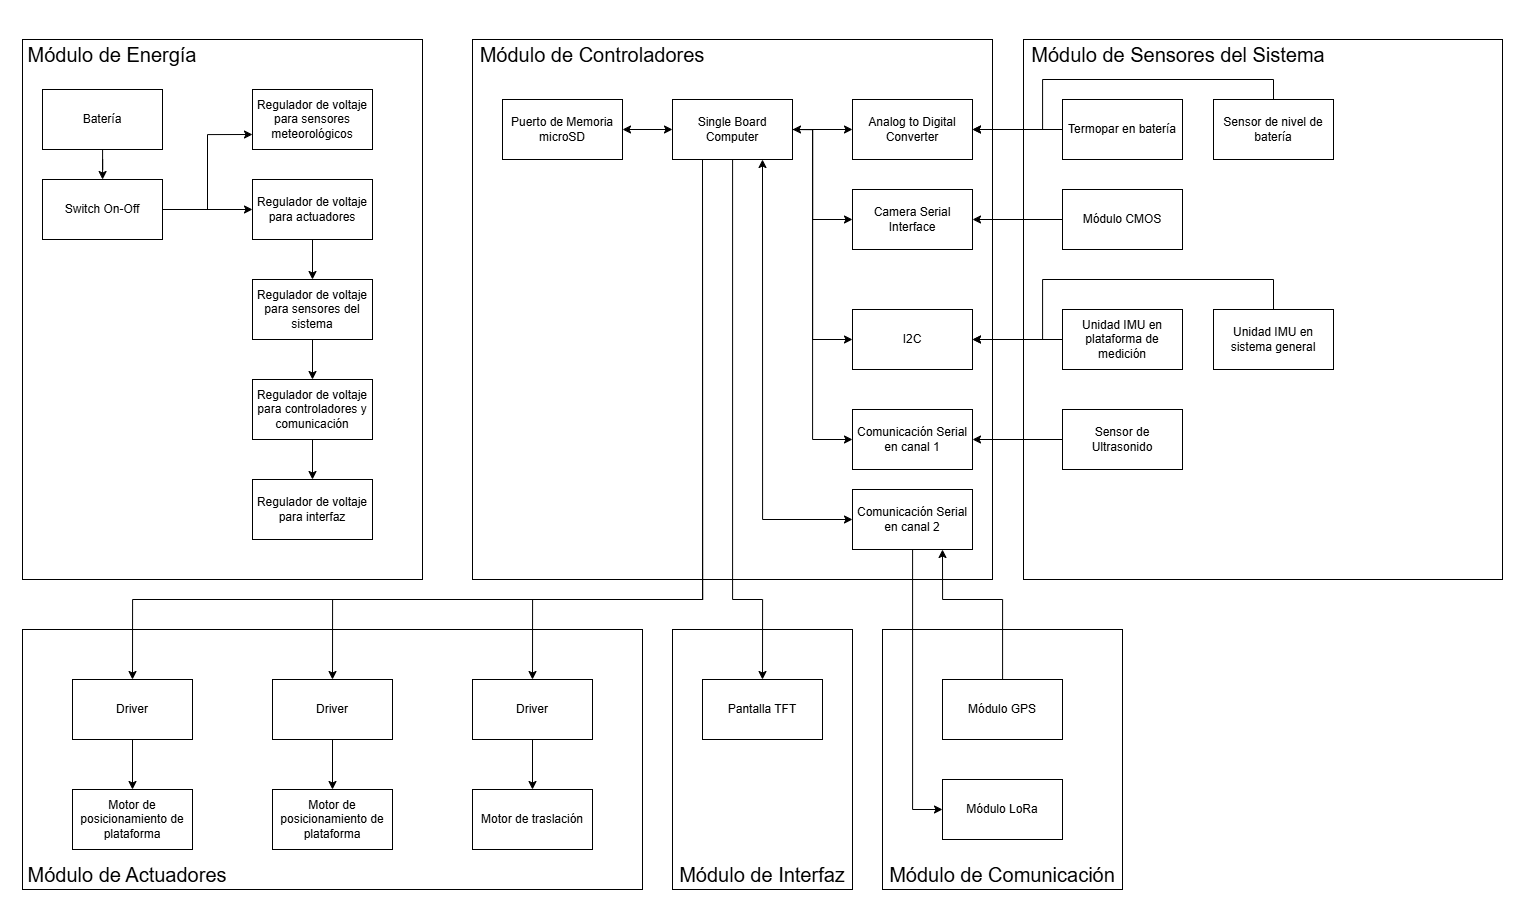
\includegraphics[width=\textwidth]{Imagenes/DiagramaBloquesTFC1_v2.png} \par\medskip
	
	\raggedright
	\footnotesize \textit{Nota.} Elaboración propia.
	\label{fig:DiagramaBloques}
\end{figure}
%%%%%
\subsection{Vista general del concepto óptimo}


\begin{figure}[H]
	% Fuerza la alineación izquierda y quita los ":" después del número
	\captionsetup{justification=raggedright, singlelinecheck=false, labelsep=none}
	
	\caption[Vista general del concepto óptimo.]{} 
	
	% Vspace negativo opcional para acercar el texto cursivo al número de figura
	\textit{Vista general del concepto óptimo.} \par\medskip
	
	\centering
	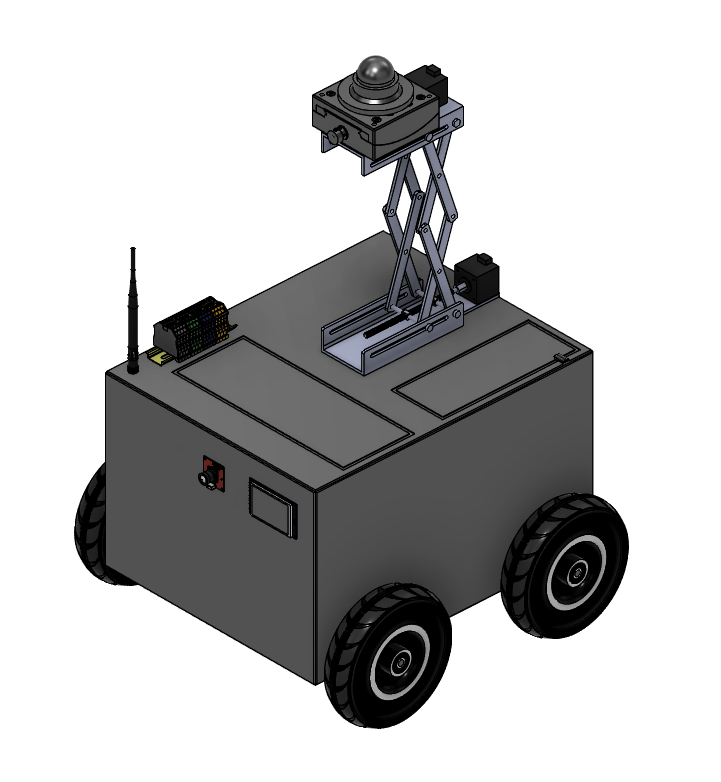
\includegraphics[width=0.6\textwidth]{Imagenes/CAD-GENERAL_V1.png} \par\medskip
	
	\raggedright
	\footnotesize \textit{Nota.} Elaboración propia.
	\label{fig:CADGENERAL}
\end{figure}

\subsection{Subsistemas mecánicos del concepto óptimo}

\subsubsection{Subsistema de traslación}

	\begin{figure}[H]
	
	\captionsetup{justification=raggedright, singlelinecheck=false, labelsep=none}
	
	\caption[Vista isometrica y frontal del subsistema de traslación.]{} 
	
	\textit{Vista isometrica y frontal del subsistema de traslación.} \par\medskip
	
	\begin{minipage}{0.5\textwidth}
		\centering
		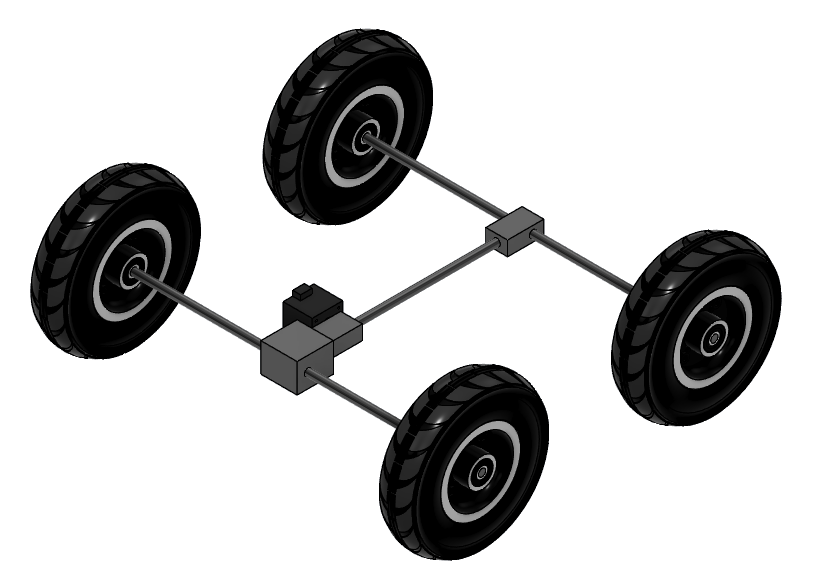
\includegraphics[width=\linewidth]{Imagenes/SISTEMA_TRASLACION_ISO.png}
	\end{minipage}\hfill
	\begin{minipage}{0.5\textwidth}
		\centering
		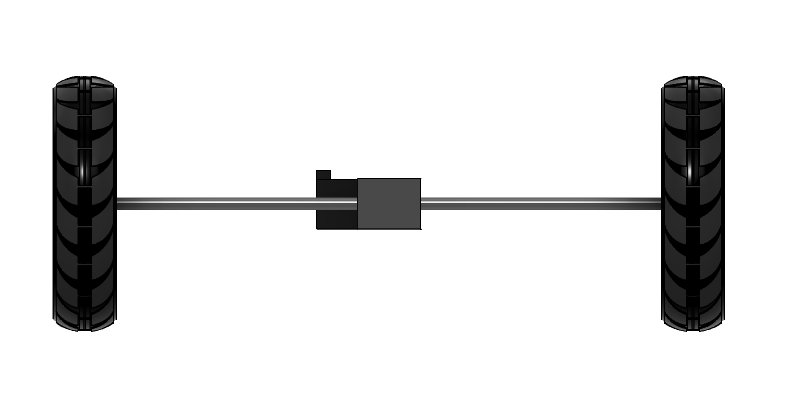
\includegraphics[width=\linewidth]{Imagenes/SISTEMA_TRASLACION_FRONT.png}
	\end{minipage}
	\par\medskip
	
	\raggedright
	\footnotesize \textit{Nota.} Elaboración propia.
	\label{fig:SubsistemaTraslacion}
\end{figure}


\subsubsection{Subsistema de posicionamiento de plataforma de medición}


\begin{figure}[H]
	
	\captionsetup{justification=raggedright, singlelinecheck=false, labelsep=none}
	
	\caption[Vista isometrica y derecha del subsistema de posicionamiento.]{} 
	
	\textit{Vista isometrica y derecha del subsistema de posicionamiento.} \par\medskip
	
	\begin{minipage}{0.5\textwidth}
		\centering
		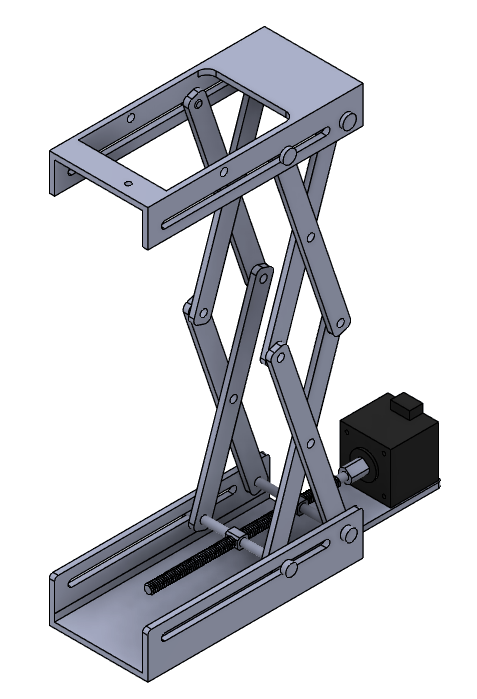
\includegraphics[width=\linewidth]{Imagenes/MECANISMO_POSICION_ISO.png}
	\end{minipage}\hfill
	\begin{minipage}{0.5\textwidth}
		\centering
		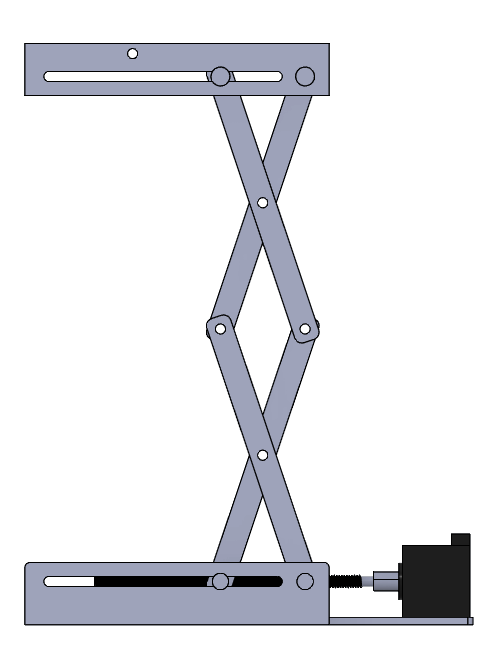
\includegraphics[width=\linewidth]{Imagenes/MECANISMO_POSICION_DERECHA.png}
	\end{minipage}
	\par\medskip
	
	\raggedright
	\footnotesize \textit{Nota.} Elaboración propia.
	\label{fig:SubsistemaPosicionamiento}
\end{figure}


\subsubsection{Subsistema de orientación de plataforma de medición}


\begin{figure}[H]
	
	\captionsetup{justification=raggedright, singlelinecheck=false, labelsep=none}
	
	\caption[Vista isometrica y derecha del subsistema de orientación.]{} 
	
	\textit{Vista isometrica y derecha del subsistema de orientación.} \par\medskip
	
	\begin{minipage}{0.5\textwidth}
		\centering
		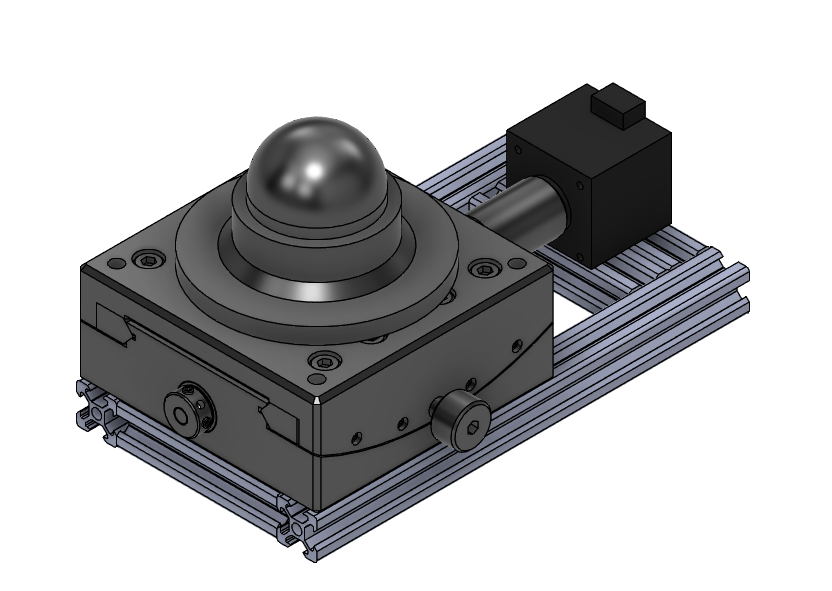
\includegraphics[width=\linewidth]{Imagenes/MECANISMO-ORIENTACION-ISO.png}
	\end{minipage}\hfill
	\begin{minipage}{0.5\textwidth}
		\centering
		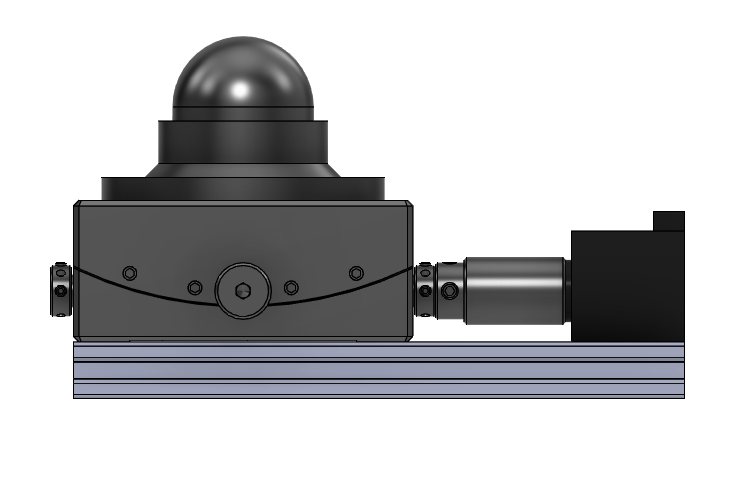
\includegraphics[width=\linewidth]{Imagenes/MECANISMO-ORIENTACION-DERECHA.png}
	\end{minipage}
	\par\medskip
	
	\raggedright
	\footnotesize \textit{Nota.} Elaboración propia.
	\label{fig:SubsistemaOrientacion}
\end{figure}

\subsubsection{Estructura de soporte}

\begin{figure}[H]
	% Fuerza la alineación izquierda y quita los ":" después del número
	\captionsetup{justification=raggedright, singlelinecheck=false, labelsep=none}
	
	\caption[Vista isométrica de la estructura.]{} 
	
	% Vspace negativo opcional para acercar el texto cursivo al número de figura
	\textit{Vista isométrica de la estructura.} \par\medskip
	
	\centering
	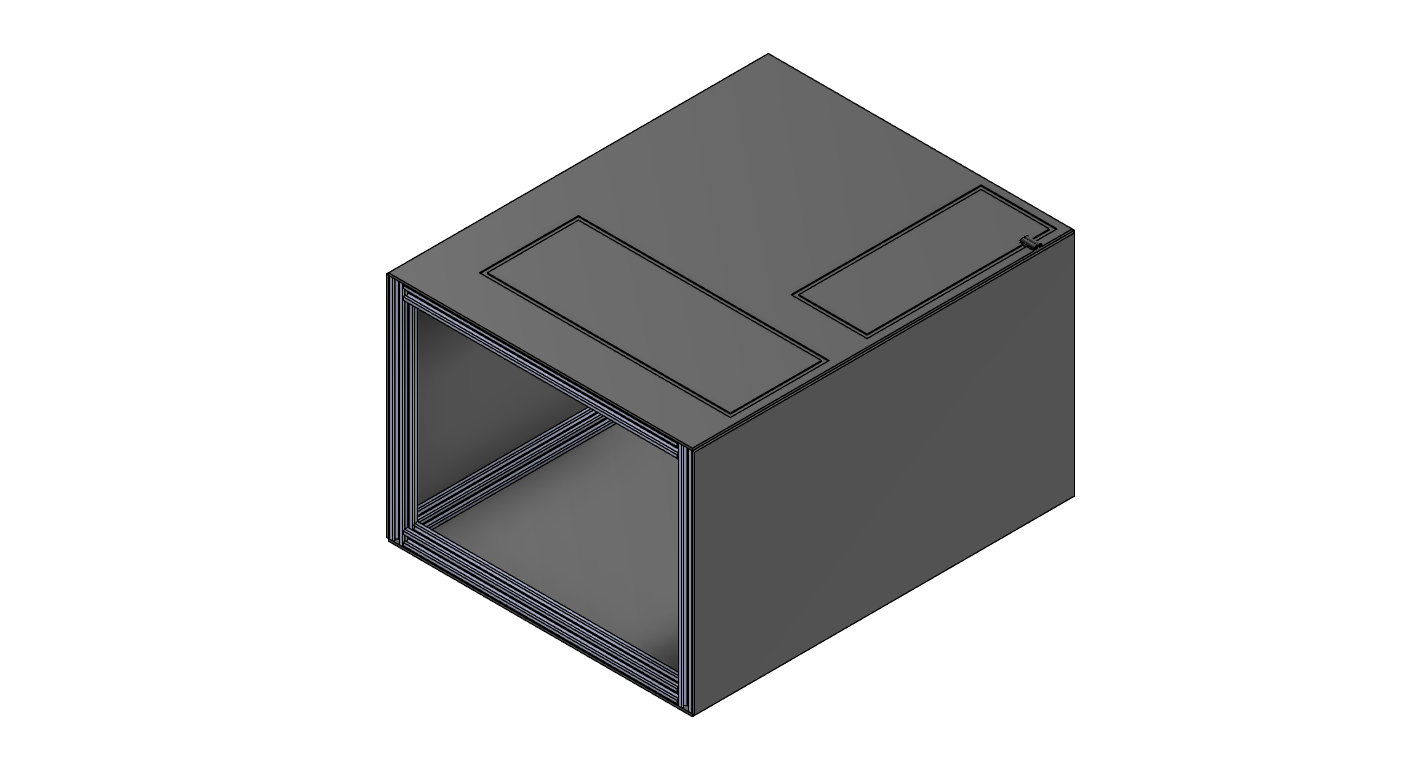
\includegraphics[width=\textwidth]{Imagenes/SOPORTE-CUBIERTA-ISO.png} \par\medskip
	
	\raggedright
	\footnotesize \textit{Nota.} Elaboración propia.
	\label{fig:CarcasaISO}
\end{figure}









%-----------------
%	Conclusiones
%-----------------

\renewcommand{\baselinestretch}{1.5}
\chapter*{\centering \large CONCLUSIONES} % No numerado, centrado
\addcontentsline{toc}{chapter}{CONCLUSIONES} 
\markboth{CONCLUSIONES}{CONCLUSIONES} % encabezado


 %Se agregan las conclusiones


%----------------------------------------------------------------------------------------
%	BIBLIOGRAFIA
%----------------------------------------------------------
%------------------------------
\newpage
%\nocite{*}
\bibliography{TFC1/biblio} %Se agrega la bibliografia
%----------------------------------------------------------------------------------------
%	Anexos
%----------------------------------------------------------------------------------------
\appendix
\renewcommand{\appendixname}{ANEXO}%
\chapter*{\appendixname}
\addcontentsline{toc}{chapter}{ANEXO} 
\markboth{ANEXO}{ANEXO} % encabezado
\thispagestyle{empty}
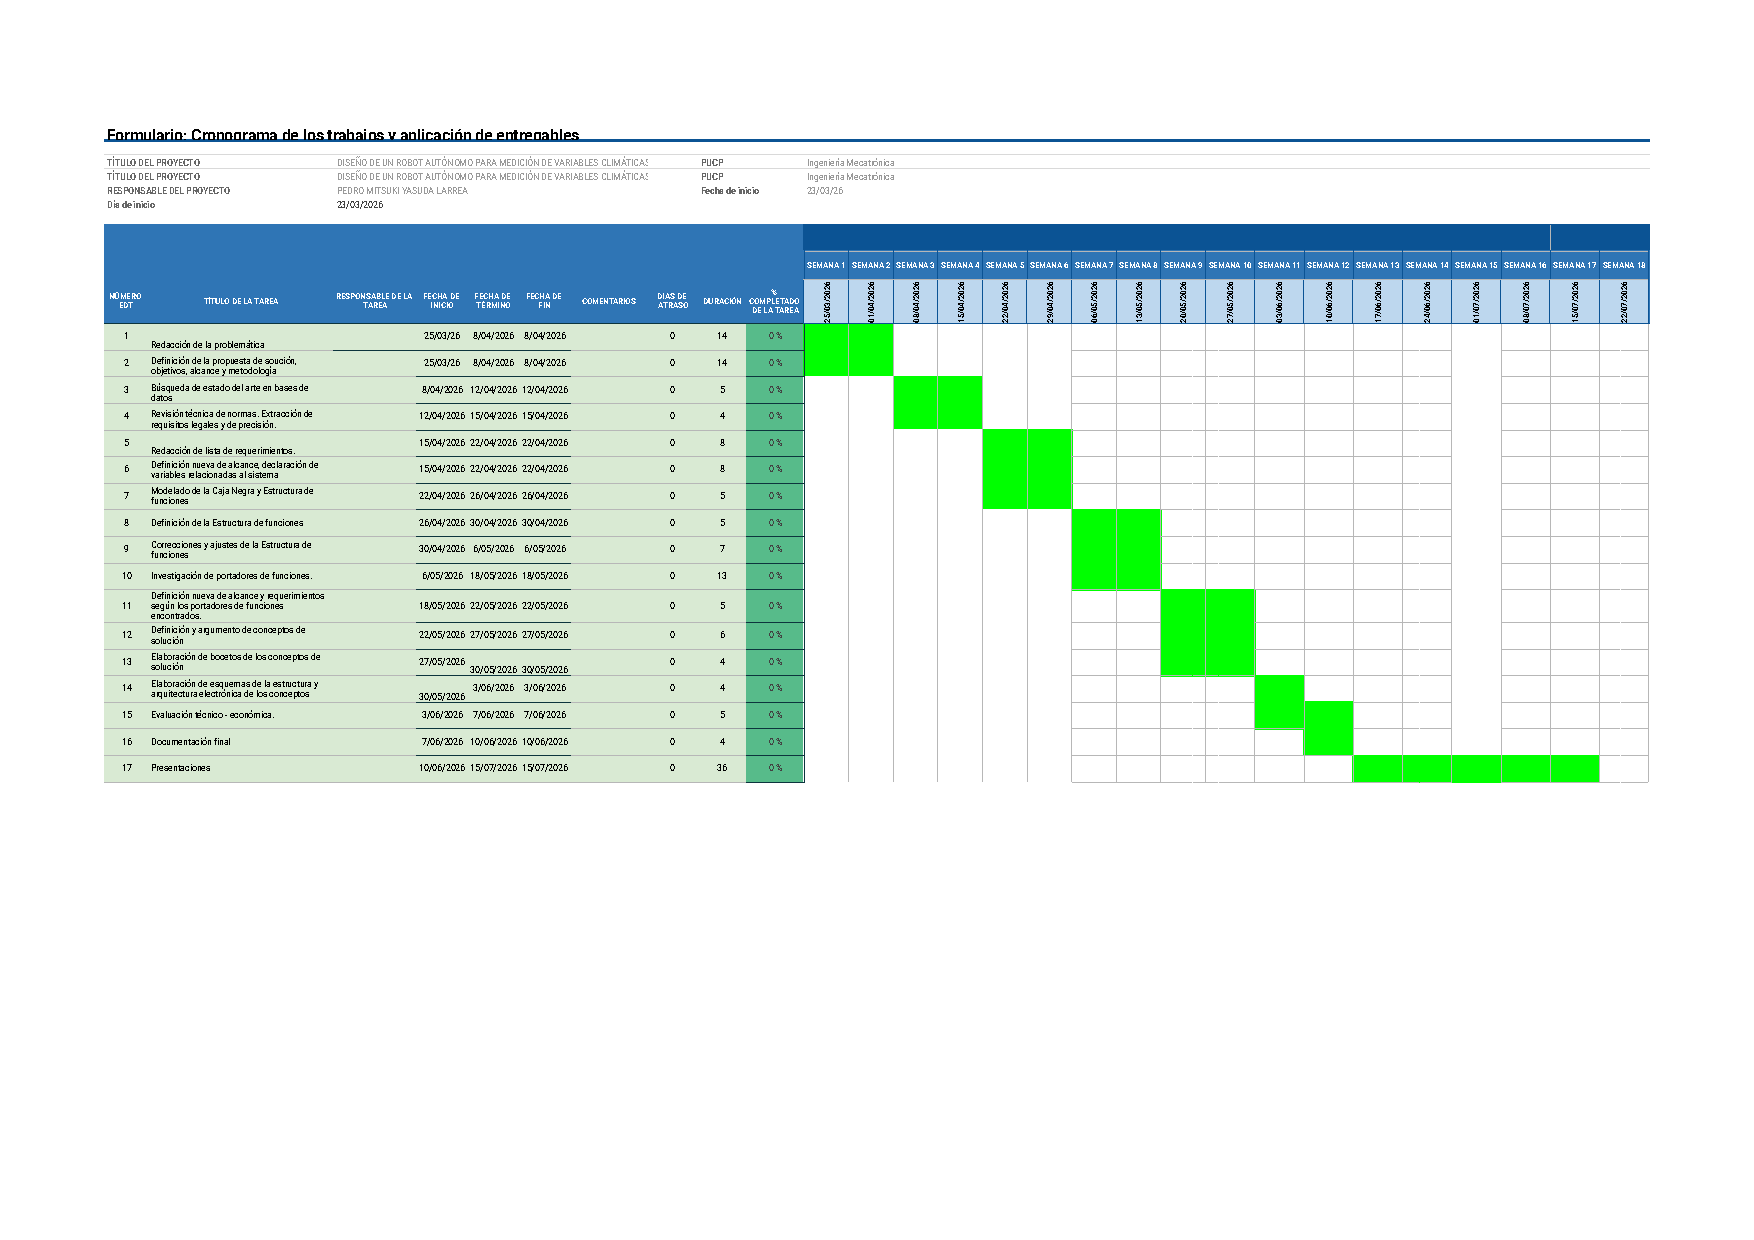
\includepdf[landscape=true, pages=-]{TFC1/DiagramaGantt.pdf}
\includepdf[pages=-]{TFC1/Avance3_EstructuraFunciones_v11.pdf}


 \phantomsection
\end{document} 


